%% MOVED TO PRO LICENSE 31 AUG 2022

%TC:ignore
\begin{filecontents*}[overwrite]{\jobname.xmpdata}
\Title{UCC School of CSIT - Bronze Departmental Award Application, December 2022}
\Author{J. Morrison et al.}
\Language{en-GB}
\Keywords{Athena Swan \sep Bronze}
\Publisher{School of Computer Science and Information Technology, University College Cork}
\Subject{Athena Swan Ireland Bronze application: Departments}
\end{filecontents*}
%TC:endignore

%% book class so we have chapters.
\documentclass[11pt,twoside]{book}

 

\usepackage{microtype}
\usepackage{sectsty}
\usepackage[utf8]{inputenc}
\usepackage[T1]{fontenc}
\usepackage[dvipsnames,table]{xcolor}
\usepackage{lettrine}
\usepackage{tabu}


\usepackage[
    paperwidth=210mm,
    paperheight=297mm,
    margin=30mm,
    includehead,includefoot
]{geometry}


\usepackage[explicit]{titlesec}
\usepackage[export]{adjustbox}


% first load package roboto to avoid other spurious warnings
\usepackage[light]{roboto}

\makeatletter
\renewcommand\seriesdefault{\mddefault\@empty}
\makeatother


\usepackage{tgschola}
%
\usepackage{setspace}
%\setstretch{1.15}

%\usepackage{float}
\usepackage{graphicx}
\usepackage{booktabs}
\usepackage{multicol}
\usepackage{multirow}
\usepackage[nointegrals]{wasysym}
\usepackage[mode=text,
            reset-text-family=false, 
            text-family-to-math=true,
            group-digits=all,
            group-minimum-digits=4,
            group-separator = {,}]{siunitx}






\definecolor{titlebgdark}{RGB}{0,112,192} %{0,163,243}
\definecolor{titlebglight}{RGB}{143,212,251}%{191,233,251}
\definecolor{darkOrange}{RGB}{80,54,16}

\usepackage{fancyhdr}
\usepackage{graphbox}

%% for un-indentation of footnotes.
\usepackage[hang,flushmargin]{footmisc}

%%% for headers we need shorter versions because the predefined chapter titles are too long. This is the magic that makes it happen.
\newcommand\chaptertitle[2]{\expandafter\def\csname=#1=\endcsname{#2}}
\newcommand\shorttitle[1]{\expandafter\csname=\leftmark=\endcsname}
\renewcommand{\chaptermark}[1]{\markboth{#1}{}}

%% DO NOT TOUCH THESE: they work as indexes I THINK.
%% Define the chapter titles here; first long, then short for the headers.
%% See https://tex.stackexchange.com/questions/627763/fancyhead-display-custom-shorten-version-of-leftmark
\chaptertitle{An introduction to the department's Athena Swan work}
             {an introduction to the department's athena swan work}

\chaptertitle{An assessment of the department's gender equality context and wider equality context}
             {the department's gender equality context and wider equality context}

\chaptertitle{Action plan}{Action plan}
%%%  end short header title.

%% needed for draft footer that states the time. XXX Remove when submitting.
\usepackage{datetime2}

\fancypagestyle{plain}{%
  \fancyhf{}%
  \fancyfoot[C]{\sffamily\color{titlebgdark}\thepage}
  \renewcommand{\headrulewidth}{0pt}%
  \renewcommand{\footrulewidth}{0pt}%
  \setlength{\headheight}{15pt}%
}

\fancypagestyle{myfancy}{%
  \fancyhf{}%
    \renewcommand{\headrulewidth}{1pt}
    \let\oldheadrule\headrule% Copy \headrule into \oldheadrule
    \renewcommand{\headrule}{\color{titlebgdark}\oldheadrule}% Add colour to \headrule

    \fancyhead[LE,RO]{\sffamily\scshape\color{titlebgdark}\thepage}
    \fancyfoot{}
    \fancyhead[LO,RE]{\sffamily\color{titlebgdark}\scshape\shorttitle{\leftmark}}
    %\fancyhead[RE,LO]{}
    \setlength{\headheight}{13.59999pt}
}

%% Remove "Chapter" / "Section" and ch/sec number from header.
\renewcommand{\chaptermark}[1]{\markboth{#1}{}}

\let\oldfrontmatter\frontmatter
\let\oldmainmatter\mainmatter
\gdef\frontmatter{\oldfrontmatter\pagestyle{plain}}
\gdef\mainmatter{\oldmainmatter\pagestyle{myfancy}}


\usepackage{framed}
\definecolor{shadecolor}{RGB}{218,227,243}
\fboxsep=8pt

%% Define SwanOrange as the color orange of the logo.
\definecolor{SwanOrange}{RGB}{244,151,8}
\definecolor{orangebg}{RGB}{249,226,193}
\definecolor{lightgray}{gray}{0.9}

%% Left align all longtables, just like normal tables
\usepackage{longtable}
\setlength{\LTleft}{0pt}

\usepackage{pifont}
%\usepackage{amssymb} 
\newcommand{\gotoactionsymbol}{\ding{43}}

\usepackage{enumitem}
\usepackage{pdflscape}
\usepackage{arydshln}
\usepackage{caption}
\usepackage{etoolbox}
\usepackage[listings,most]{tcolorbox}


\tcbuselibrary{breakable}



\captionsetup[figure]{labelfont={color=black,bf,sf},
                      textfont={color=black,sf},
                      singlelinecheck=off,
                      justification=raggedright,
                      labelsep=space
}
                      
\captionsetup[table]{labelfont={color=black,bf,sf},
                     textfont={color=black,sf},
                     singlelinecheck=off,
                     justification=raggedright,
                     labelsep=space
}

\captionsetup[longtable]{labelfont={color=black,bf,sf},
                     textfont={color=black,sf},
                     singlelinecheck=off,
                     justification=raggedright,
                     labelsep=space
}

%% change some settings to get dotted lines, not dashed lines, between table rows.
\setlength{\dashlinedash}{0.5pt}
\setlength{\dashlinegap}{4.5pt}
\setlength{\arrayrulewidth}{.5pt}

%% change spacing of main text.
\renewcommand\baselinestretch{1.2}

%% Define an indented paragraph; 6mm is the indentation of the subsubsections.
\usepackage{changepage} 
\newenvironment{indentedparagraph}{%
    \begin{adjustwidth}{6mm}{}}{\end{adjustwidth}}

% command for auxiliary instruction text including itemized lists.
\newcommand{\instr}[1]{
\vspace{-16pt}
\begin{indentedparagraph}
\singlespacing
\color{titlebgdark}\sffamily{#1}
\end{indentedparagraph}
\vspace{5mm}
}



%% Separation of paragraphs: no indent, bit of vspace.
\setlength{\parskip}{7pt}
\setlength{\parindent}{0cm}


%% Remove page numbers on empty pages (e.g. the empty pages before a chapter)
\let\origdoublepage\cleardoublepage
\newcommand{\clearemptydoublepage}{\clearpage{\pagestyle{empty}\origdoublepage}}
\let\cleardoublepage\clearemptydoublepage
%% End remove page numbers.

% We're using documentclass book, which defines chapters, but we're calling them sections. beware of this hack. XXX HACK 
\renewcommand{\chaptername}{Section}
\chapterfont{\color{titlebgdark}\sffamily\raggedright} 
\sectionfont{\color{titlebgdark}\sffamily\raggedright}
\subsectionfont{\color{titlebgdark}\sffamily\mdseries\fontsize{11}{12}\selectfont}
\subsubsectionfont{\color{titlebgdark}\sffamily}
\paragraphfont{\color{darkOrange}\sffamily\bfseries}

%% Redefine subsections as the alpha-numbered elements (a, b, c)
\renewcommand\thesubsection{\alph{subsection}}

%% Reformat subsections so that they are not that big.
%\titleformat{\subsection}{\color{SwanOrange}\sffamily\fontsize{12}{15}}{\thesubsection.}{1em}{}

%% Remove chapter number from the sections' numbers (so, not "2.3 xyz", but "3 xyz")
\renewcommand\thesection{\arabic{section}}

%%%



%% Make orange + character for itemization/bullet point.
\renewcommand\labelitemi{\color{SwanOrange}{\textbf{+}}}
\setlist[itemize]{itemsep=1pt}

%% Stretch out vertically a bit for tables
\renewcommand{\arraystretch}{1.5}

%% Stuff we need for the orange border on front cover.
\usepackage{eso-pic}
\usepackage{calc}
\newlength\myborder
\myborder=40pt %% <--- defines width of the orange border.
%% end front cover.

%% To enable 3-part action numbering:
\newcounter{actioncounter}
\setcounter{actioncounter}{1}



%% formatting of the table of contents
\usepackage[titles]{tocloft}

\cftsetindents{section}{2em}{2.5em}
\cftsetindents{subsection}{2em}{3.5em}

%% Make the TOC a bit tighter so it fits on 1 page.
\renewcommand\cftchapafterpnum{\vskip-3pt}
\renewcommand\cftsecafterpnum{\vskip-1pt}

\makeatletter
% add tcblistings to \jobname.lol (list of listings)
\tcbset{
  addtolol/.style={list entry={\kvtcb@title},
  add to list={lol}{subsection}},
}
\makeatother



\newtcbtheorem[auto counter,
               number within=chapter,
               number freestyle={\noexpand\thechapter{}.\noexpand\thesection{}.\noexpand\theactioncounter}, % three-part action numbering               
               list inside={thm}]%
    {actionblock}%    
    {ACTION}%
    {        
        fonttitle=\sffamily\bfseries\footnotesize,
        fontupper=\sffamily,
        sharp corners,
        left=2mm,
        top=2mm,
        bottom=1mm,
        right=1mm,
        enhanced,
        boxrule=0mm,
        borderline west={3pt}{0pt}{RoyalBlue},
        colback=titlebglight!30!white,
        colframe=titlebglight!30!white,
        coltitle=titlebgdark,
        code={\singlespacing\stepcounter{actioncounter}},
        after skip=20pt plus 2pt
    }%
    {action}

\makeatletter
\newcommand{\ttll@actionblock}{-1000}
\makeatother


\newtcbtheorem{UCCaction}{\textsf{UCC INSTITUTIONAL ATHENA SWAN BRONZE AWARD ACTION \textsf{#1}}}{%
        theorem name,%
        separator sign={ },
        colback=green!15,%
        colframe=green!15,
        coltitle=green!35!black,
        borderline west={3pt}{0pt}{green!35!black},
        sharp corners,
        left=2mm,
        top=2mm,
        bottom=1mm,
        right=1mm,
        enhanced,
        arc=0pt,
        outer arc=0pt,
        enhanced,
        fonttitle=\sffamily\bfseries\footnotesize,
        fontupper=\sffamily,
        boxrule=0mm,   
        after skip=20pt plus 2pt
    }%
    {UCCaction}


\newtcolorbox{priority}[2][]
{
    arc=0pt,
    outer arc=0pt,    
    fonttitle=\sffamily\bfseries\footnotesize,
    fontupper=\sffamily,
    sharp corners,
    left=2mm,
    top=2mm,
    bottom=1mm,
    right=1mm,
    enhanced,
    boxrule=0mm,
    borderline west={3pt}{0pt}{SwanOrange!35!black},
    colback  = SwanOrange!10,%
    colframe = SwanOrange!10,%        
    coltitle = darkOrange,%        
    title    = {PRIORITY \hypertarget{priority:#2}{#2}},
    #1
}


%% Reset action counter whenever a new chapter or section starts
%% to support three-part action numbering.
\makeatletter
\@addtoreset{actioncounter}{chapter}
\@addtoreset{actioncounter}{section}
\@addtoreset{figure}{section} %% reset figure counter for each new section
\@addtoreset{table}{section}  %% reset table counter for each new section
\makeatother

%% 3-part numbering of figures and tables. CHAPTER.SECTION.counter
\renewcommand{\thetable}{\arabic{chapter}.\arabic{section}.\arabic{table}}   
\renewcommand{\thefigure}{\arabic{chapter}.\arabic{section}.\arabic{figure}}   

\newtcolorbox{prompt}{%
    colback=titlebgdark!5,
    coltext=titlebgdark,
    arc=0pt,
    outer arc=0pt,
    enhanced,
    boxrule=0.5pt,
    colframe=titlebgdark
}


\newenvironment{longfigure}
  {\renewcommand\LTcaptype{figure}\longtable}
  {\endlongtable}

%% Ignore all instruction text and environments as listed below. Also ignore quotes. 
%TC:macro \instr 1
%TC:macro \todo 1 

%TC:envir myquote 0 0 
%TC:envir prompt 0 0 
%TC:envir action 0 0 
%TC:envir UCCaction 0 0
%TC:envir figbox 0 0 
%TC:envir tabbox 0 0 
%TC:envir table 0 0 
%TC:envir figure 0 0 
%TC:envir longtable 0 0 
%TC:envir longfigure 0 0 
%TC:envir SCfigure 0 0
%TC:envir titlepage 0 0 



\AtBeginEnvironment{letter}{\footnotesize}

\usepackage{tikz}
\newcommand\quotesize{60} 
\newcommand{\myopenquote}{\tikz[remember picture,overlay,xshift=-5.5ex,yshift=-2.5ex]
  \node (OQ) {\normalfont\fontsize{\quotesize}{\quotesize}\selectfont``};\kern0pt}


   
\newtcolorbox{myquote}{%
    arc=0pt,
    outer arc=0pt,
    enhanced,
    boxrule=0.5pt,    
    coltext=black,
    colframe=white,
    colback=white,
    left=40pt,
    right=30pt,
    fontupper=\rmfamily\small\itshape 
}

% could change colour of table lines     
%\arrayrulecolor{RoyalBlue} 

% KS to replace p{2cm}; now P{2cm} with right-justified text.
\newcolumntype{P}[1]{>{\raggedright\arraybackslash}p{#1}}
\newcolumntype{M}[1]{>{\raggedright\arraybackslash}m{#1}}
% KS column type for right-aligned text (e.g. numbers)
\newcolumntype{R}[1]{>{\raggedleft\arraybackslash}p{#1}}
\newcolumntype{C}[1]{>{\centering\arraybackslash}p{#1}}



%%% Magic to change font for tables automatically.
\makeatletter
\providecommand*\AtBeginEnvironment[1]{%
  \@ifundefined{#1}%
    {\@latex@error{Environment #1 undefined}\@ehc
     \@gobble}%
    {\@ifundefined{ABE@env@#1}%
       {\expandafter\let\csname ABE@env@#1\expandafter\endcsname
          \csname #1\endcsname
        \expandafter\let\csname ABE@hook@#1\endcsname\@empty
        \@namedef{#1}{\@nameuse{ABE@hook@#1}\@nameuse{ABE@env@#1}}}%
       {}%
     \expandafter\g@addto@macro\csname ABE@hook@#1\endcsname}}
\@onlypreamble\AtBeginEnvironment
\makeatother

\AtBeginEnvironment{tabular}{\sffamily}
\AtBeginEnvironment{tabu}{\sffamily}
\AtBeginEnvironment{longtable}{\sffamily}
\AtBeginEnvironment{longfigure}{\sffamily}

%%% End Magic



%% code for the fancy chapter headings. 
\titleformat{\chapter}[display]
  {\normalfont\huge\bfseries}
  {}
  {20pt}
  {%
    \begin{tcolorbox}[
      enhanced,
      colback=titlebgdark,
      boxrule=0.25cm,
      colframe=titlebglight,
      arc=0pt,
      outer arc=0pt,
      leftrule=0pt,
      rightrule=0pt,
      fontupper=\color{white}\sffamily\bfseries\huge,
      enlarge left by=-1in-\hoffset-\oddsidemargin, 
      enlarge right by=-\paperwidth+1in+\hoffset+\oddsidemargin+\textwidth,
      width=\paperwidth, 
      left=1in+\hoffset+\oddsidemargin, 
      right=\paperwidth-1in-\hoffset-\oddsidemargin-\textwidth,
      top=0.6cm, 
      bottom=0.6cm,
      overlay={
        \node[
          fill=titlebgdark,
          draw=titlebglight,
          line width=0.15cm,
          inner sep=0pt,
          text width=1.7cm,
          minimum height=1.7cm,
          align=center,
          font=\color{white}\sffamily\bfseries\fontsize{30}{36}\selectfont
        ] 
        (chapname)
        at ([yshift=13mm,xshift=-17cm]frame.north east)
        %at ([yshift=3mm,xshift=-4cm]frame.north east)
        {\thechapter};
        \node[font=\small,anchor=south,inner sep=2pt] at (chapname.north)
        {};  % if using amsbook, this should be \chaptername
      } 
    ]
    #1
    \end{tcolorbox}%
  }
\titleformat{name=\chapter,numberless}[display]
  {\normalfont\huge\bfseries}
  {}
  {20pt}
  {%
    \begin{tcolorbox}[
      enhanced,
      colback=titlebgdark,
      boxrule=0.25cm,
      colframe=titlebglight,
      arc=0pt,
      outer arc=0pt,
      remember as=title,
      leftrule=0pt,
      rightrule=0pt,
      fontupper=\color{white}\sffamily\bfseries\huge,
      enlarge left by=-1in-\hoffset-\oddsidemargin, 
      enlarge right by=-\paperwidth+1in+\hoffset+\oddsidemargin+\textwidth,
      width=\paperwidth, 
      left=1in+\hoffset+\oddsidemargin, 
      right=\paperwidth-1in-\hoffset-\oddsidemargin-\textwidth,
      top=0.6cm, 
      bottom=0.6cm, 
    ]
    #1
    \end{tcolorbox}%
  }
\titlespacing*{\chapter}
  {0pt}{0pt}{40pt}
%\makeatother




%% HACK: until figure out how \tcblistof{} can add more space between ID and title, this works.
\newcommand{\ksspace}{\hspace{1em}}

\usepackage{subcaption}

\renewcommand{\cftchapfont}{\sffamily\bfseries}
\renewcommand{\cftsecfont}{\sffamily}
% change font for page numbers
\renewcommand{\cftchappagefont}{\sffamily\bfseries}
\renewcommand{\cftsecpagefont}{\sffamily}

% list of fig/tab entries and page numbers
\renewcommand{\cftfigfont}{\sffamily}
\renewcommand{\cfttabfont}{\sffamily}
\renewcommand{\cftfigpagefont}{\sffamily}
\renewcommand{\cfttabpagefont}{\sffamily}


\setlength{\cftfignumwidth}{3em}
\setlength{\cfttabnumwidth}{3em}


% this package includes the list of tables and list of figures to the ToC.
\usepackage[nottoc]{tocbibind}

%%%%%%%%%%%%%%%%%%%%%%%%%%%%%%%%%%%%%%%%%%%%%%%%%%%%%%%%%%%%%%%%%%%%

\usepackage{makeidx} 
\makeindex 

%% allows newlines in single table cells using \makecell command
\usepackage{makecell}


\newcommand{\interdis}{$\star$}

%%% spacing after section titles.
%% https://tex.stackexchange.com/questions/53338/reducing-spacing-after-headings
%% \titlespacing*{<command>}{<left>}{<before-sep>}{<after-sep>}
\titlespacing\subsection{0pt}
                        {36pt plus 4pt minus 2pt}
                        {12pt plus 2pt minus 2pt}
\titlespacing\subsubsection{0pt}
                           {12pt plus 4pt minus 2pt}
                           {-4pt plus 2pt minus 2pt}
% spacing: how to read {12pt plus 4pt minus 2pt}
%           12pt is what we would like the spacing to be
%           plus 4pt means that TeX can stretch it by at most 4pt
%           minus 2pt means that TeX can shrink it by at most 2pt
%       This is one example of the concept of, 'glue', in TeX

%% end spacing after section titles.

%% specify what the symbol looks like in the action boxes that links to the big action table.



%% read all acronym definitions
\usepackage{acro}

%% specify what the terms & acronyms table looks like.
\acsetup{format/short=\textmd,
         format/long       =\textmd,
         list/template     = longtable,
         patch/longtable   = false,
         templates/colspec = {@{}p{3cm}p{12cm}@{}},
         list/display      = all
}



%% Load all acronyms and terms.
%%
%% Alphabetic order please!
%%
%%

%TC:ignore

%% A

\DeclareAcronym{ADVANCE}{
  short = ADVANCE-CRT,
  long  = The SFI Centre for Research Training for Advanced Networks for Sustainable Societies,
  tag   = A
}

\DeclareAcronym{AS}{
  short = AS,
  long  = Athena Swan,
  tag   = A
}


\DeclareAcronym{APCD}{
    short = APCD,
    long  = Academic Programmes and Curriculum Development,
    tag   = A
}

%% B

\DeclareAcronym{BA}{
  short = BA,
  long  = Bachelor of Arts,
  tag   = A
}

\DeclareAcronym{BADH}{
  short = BADH,
  long  = BA in Digital Humanities,
  tag   = A
}



\DeclareAcronym{BSc}{
  short = BSc,
  long  = Bachelor of Science,
  tag   = A
}

\DeclareAcronym{BScCS}{
  short = BScCS,
  long  = BSc in Computer Science,
  tag   = A
}

\DeclareAcronym{BScDSA}{
  short = BScDSA,
  long  = BSc in Data Science and Analytics,
  tag   = A
}


\DeclareAcronym{BAPC}{
  short = BAPC,
  long  = BA in Psychology and Computing,
  tag   = A
}

%% C

\DeclareAcronym{CAS}{
  short = CAS,
  long  = Central Academic Services,
  tag   = A
}

\DeclareAcronym{CID}{
  short = CID,
  long  = Contract of Indefinite Duration,
  tag   = A
}
\DeclareAcronym{CIRTL}{
  short = CIRTL,
  long  = {Centre for Integration of Research, Teaching, and Learning},
  tag   = A
}


\DeclareAcronym{Confirm}{
  short = Confirm,
  long  = The SFI Research Centre for Smart Manufacturing,
  tag   = A
}

\DeclareAcronym{Connect}{
  short = Connect,
  long  = The SFI Research Centre for Future Networks and Communications,
  tag   = A
}

\DeclareAcronym{CRT}{
  short = CRT,
  long  = Centre for Research Training,
  tag   = A
}

\DeclareAcronym{CRT-AI}{
  short = CRT-AI,
  long  = The SFI Centre for Research Training in Artificial Intelligence,
  tag   = A
}

\DeclareAcronym{CSIT}{
  short = CSIT,
  long  = School of Computer Science and Information Technology,
  tag   = A
}

\DeclareAcronym{CS}{
  short = CS,
  long  = Computer Science,
  tag   = A
}


\DeclareAcronym{CSSS}{
  short = CSSS,
  long  = Computer Science Systems Support,
  tag   = A
}

%% D

\DeclareAcronym{DCU}{
  short = DCU,
  long  = {Dublin City University},
  tag   = A
}


\DeclareAcronym{DEIS}{
  short = DEIS,
  long  = {Delivering Equality of opportunity In Schools; a category of schools that meet certain disadvantage criteria, as defined on the Department of Education website: \url{https://www.gov.ie/en/publication/a3c9e-extension-of-deis-to-further-schools/}},
  tag   = A
}


\DeclareAcronym{DISC}{
  short = DISC,
  long  = Disciplines Inquiring into Societal Challenges,
  tag   = A
}



\DeclareAcronym{DSS}{
  short = DSS,
  long  = Disability Support Services,
  tag   = A
}


%% E


\DeclareAcronym{EDI}{
  short = EDI,
  long  = {Equality, Diversity, and Inclusion},
  tag   = A
}

\DeclareAcronym{EDIIC}{
    short = EDIIC,
    long  = EDI Implementation Committee,
    tag   = A
}

\DeclareAcronym{Enable}{
  short = Enable,
  long  = {Science Foundation Ireland Spoke on Smart Communities involving Connect, Lero, and Insight},
  tag   = A
}

%% F

\DeclareAcronym{F}{
  short = F,
  long  = Female,
  tag   = A
}


\DeclareAcronym{FTE}{
  short = FTE,
  long  = Full Time Equivalent,
  tag   = A
}


%% H

\DeclareAcronym{HDACT}{
  short = HDACT,
  long  = Higher Diploma in Applied Computer Technology,
  tag   = A
}


\DeclareAcronym{HE}{
  short = HE,
  long  = Higher Education,
  tag   = A
}

\DeclareAcronym{HEA}{
  short = HEA,
  long  = Higher Education Authority (Ireland),
  tag   = A
}

\DeclareAcronym{HeCoS}{
  short = HeCoS,
  long  = Higher Education Classification of Subjects,
  tag   = A
}


\DeclareAcronym{HESA}{
  short = HESA,
  long  = Higher Education Statistics Agency (UK),
  tag   = A
}


\DeclareAcronym{HOS}{
  short = HoS,
  long  = Head of School,
  tag   = A
}

\DeclareAcronym{HR}{
  short = HR,
  long  = Department of Human Resources,
  tag   = A
}


%% I

\DeclareAcronym{ICT}{
  short = ICT,
  long  = Information and Communication Technologies,
  tag   = A
}


\DeclareAcronym{IHREC}{
  short = IHREC,
  long  = Irish Human Rights and Equality Commission,
  tag   = A
}


\DeclareAcronym{Insight}{
  short = Insight,
  long  = Insight SFI Research Centre for Data Analytics,
  tag   = A
}

\DeclareAcronym{IO}{
  short = IO,
  long  = International Office,
  tag   = A
}


\DeclareAcronym{ISCED}{
  short = ISCED,
  long  = International Standard Classification of Education,
  tag   = A
}


\DeclareAcronym{iWish}{
  short = iWish,
  long  = {I WISH is a Volunteer led community committed to showcasing the power of Science, Technology, Engineering and Maths to female secondary school students},
  tag   = A
}

%% L
\DeclareAcronym{Lero}{
  short = Lero,
  long  = The SFI Research Centre for Software,
  tag   = A
}

%% M

\DeclareAcronym{M}{
  short = M,
  long  = Male,
  tag   = A
}

\DeclareAcronym{MU}{
  short = MU,
  long  = Maynooth University,
  tag   = A
}



\DeclareAcronym{MPT}{
  short = MPT,
  long  = Munster Programming Training,
  tag   = A
}

\DeclareAcronym{MSc}{
  short = MSc,
  long  = Master of Science,
  tag   = A
}

\DeclareAcronym{MScIM}{
  short = MScIM,
  long  = MSc in Interactive Media,
  tag   = A
}


\DeclareAcronym{MScDSA}{
  short = MScDSA,
  long  = MSc in Data Science and Analytics,
  tag   = A
}

\DeclareAcronym{MScCS}{
  short = MScCS,
  long  = MSc in Computer Science,
  tag   = A
}



%% O

\DeclareAcronym{OVPRI}{
    short = OVPRI,
    long  = Office of the VP for Research and Innovation,
    tag   = A
}

%% P

\DeclareAcronym{PGT}{
  short = PGT,
  long  = {Postgraduate Taught students},
  tag   = A
}

\DeclareAcronym{PGR}{
  short = PGR,
  long  = {Postgraduate Research student},
  tag   = A
}


\DeclareAcronym{PI}{
  short = PI,
  long  = Principal Investigator,
  tag   = A
}


\DeclareAcronym{PMS}{
  short = PMS,
  long  = Professional Management and Support,
  tag   = A
}

\DeclareAcronym{PMSS}{
  short = PMSS,
  long  = Professional Management and Support Staff,
  tag   = A
}

\DeclareAcronym{PDR}{
  short = PDR,
  long  = Performance Development Review,
  tag   = A
}

\DeclareAcronym{PDRS}{
  short = PDRS,
  long  = Performance Development Review System,
  tag   = A
}


%% S

\DeclareAcronym{SALI}{
  short = SALI,
  long  = {Strategic Academic Leadership Initiative},
  tag   = A
}

\DeclareAcronym{SAT}{
  short = SAT,
  long  = Self-Assessment Team,
  tag   = A
}

\DeclareAcronym{SEFS}{
  short = SEFS,
  long  = {Science, Engineering, and Food Science},
  tag   = A
}

\DeclareAcronym{SFI}{
  short = SFI,
  long  = Science Foundation Ireland,
  tag   = A
}

\DeclareAcronym{SIPTU}{
  short = SIPTU,
  long  = {Services, Industrial, Professional and Technical Union},
  tag   = A
}

\DeclareAcronym{SL}{
  short = SL,
  long  = {Senior Lecturer},
  tag   = A
}


\DeclareAcronym{STEM}{
  short = STEM,
  long  = {Science, Technology, Engineering, and Mathematics},
  tag   = A
}


%% T

\DeclareAcronym{TCD}{
  short = TCD,
  long  = Trinity College Dublin,
  tag   = A
}


\DeclareAcronym{TLCF}{
    short = TLCF,
    long  = Third Level Computing Forum,
    tag   = A
} 

\DeclareAcronym{TLSE}{
    short = TLSE,
    long  = Teaching Learning and Student Experience,
    tag   = A
}

%% U

\DeclareAcronym{UCC}{
  short = UCC,
  long  = University College Cork,
  tag   = A
}

\DeclareAcronym{UCD}{
  short = UCD,
  long  = University College Dublin,
  tag   = A
}

\DeclareAcronym{UK}{
  short = UK,
  long  = United Kingdom,
  tag   = A
}

%% W

\DeclareAcronym{WG}{
  short = WG,
  long  = Workgroup,
  tag   = A
}

\DeclareAcronym{WGs}{
  short = WGs,
  long  = Workgroups,
  tag   = B
}



\DeclareAcronym{WiSTEM}{
  short = WiSTEM,
  long  = Women in STEM,
  tag   = A
}

%TC:endignore






%% Mark TODOs XXX Remove this when submitting
%%\newcommand\todo[1]{\textcolor{red}{#1}}


% hyperlink settings go here.
\usepackage{hyperref}
\hypersetup{
    hypertexnames=false,  %% Not entirely sure what this does but it seems to fix a problem with the hyperlinks in the list of actions.
    colorlinks=true,   
    citecolor=black,
    urlcolor=black,
    linkcolor=titlebgdark,
    bookmarksnumbered=true,     
    bookmarksopen=true,         
    bookmarksopenlevel=1,       
    colorlinks=true,            
    pdfstartview=Fit,           
    pdfpagemode=UseOutlines,    
    pdfpagelayout=TwoPageRight
}

%\renewcommand{\theHsection}{\thechapter.section.\thesection}


% \usepackage{cleveref}

% \newtcblisting[auto counter,
%                number within=chapter,
%                %crefname={lis.}{lis.},
%                %Crefname={Listing}{Listings},
%                number freestyle={\noexpand\thechapter{}.\noexpand\thesection{}.\noexpand\theactioncounter},
%                list inside=lis,
%               ]{labelboxcode}[3][]{%
%     listing options={#1},    
%     comment={#3},
%     label=#2,
%     arc=0pt,
%     outer arc=0pt,    
%     title=ACTION~\thetcbcounter,
%     fonttitle=\sffamily\bfseries\footnotesize,
%     fontupper=\sffamily,
%     fontlower=\sffamily,
%     sharp corners,
%     left=2mm,
%     top=2mm,
%     bottom=1mm,
%     right=1mm,
%     enhanced,
%     boxrule=0mm,
%     borderline west={3pt}{0pt}{RoyalBlue},
%     colback=titlebglight!30!white,
%     colframe=titlebglight!30!white,
%     coltitle=titlebgdark,
%     code={\singlespacing\stepcounter{actioncounter}},
%     after skip=20pt plus 2pt,        
%     comment only
% }

%% Consult https://texblog.net/hyperref/
%% These packages have to be loaded after hyperref.
%% captions on the side of a table. 
%%\usepackage{sidecap}
\usepackage{ragged2e}
\usepackage{mdframed}
\usepackage{nicefrac}
%%%%%%%%%%%%%%%%%%%%%%%%

%%%%%%%%%%%%%%%%%%%
%% We don't need to load pdfx package, apparently. but if we do, then after hyperref.
%\usepackage[a-1b]{pdfx}


\newcommand\crule[3][titlebgdark]{\textcolor{#1}{\rule{#2}{#3}}}

\newsavebox{\tempbox}
\newenvironment{figbox}[2][\dimexpr\columnwidth-2\fboxsep\relax]
  {
    \begin{figure}[#2]
    \begin{lrbox}{\tempbox}%
        \begin{minipage}{#1}
        \vspace{-8pt}
        \crule{12mm}{3mm}
  }
  {
    \end{minipage}
    \end{lrbox}%
    \colorbox{orangebg}{\usebox{\tempbox}}
    \end{figure}
  }
  
\newenvironment{tabbox}[2][\dimexpr\columnwidth-2\fboxsep\relax]
  {
    \begin{table}[#2]
    \begin{lrbox}{\tempbox}%
        \begin{minipage}{#1}
        \vspace{-8pt}
        \crule{12mm}{3mm}
  }
  {
    \end{minipage}
    \end{lrbox}%
    \colorbox{orangebg}{\usebox{\tempbox}}
    \end{table}
  }


\usepackage{ifthen,changepage}

%%%%%%%%%%%%%%%%%%%%%%%%%%%%%%%%%%%%%%%%%%%%%%%%%%%%%%%%%%%%%%%%%%%%%%%%%%%%%%%%%%%%%%%%%%%
%%%%%%%%%%%%%%%%%%%%%%%%%%%%%%%%%%%%%%%%%%%%%%%%%%%%%%%%%%%%%%%%%%%%%%%%%%%%%%%%%%%%%%%%%%%
%%%%%%%%%%%%%%%%%%%%%%%%%%%%%%%%%%%%%%%%%%%%%%%%%%%%%%%%%%%%%%%%%%%%%%%%%%%%%%%%%%%%%%%%%%%


\begin{document}

%TC:ignore
\frontmatter

%% Define the front cover here.
\begin{titlepage}

    \newgeometry{left=65pt,right=30pt,bottom=30pt,top=60pt}
    
    %% add an orange border. Don't ask me what it does, it's from the web.
    {   \pagecolor{SwanOrange}
        \AddToShipoutPictureBG*
        {%
            \AtPageLowerLeft
            {%
                \color{white}%
                \hspace{\myborder}%
                \rule[\myborder]{\paperwidth-2\myborder}{\paperheight-2\myborder}%
            }%
        }
    }
    %% end orange border.

    %% positioning of the two logos. 
    \begin{tabular}{p{0.5\textwidth} p{0.5\textwidth}}
        \vspace{0pt} 
        
\includegraphics[trim={3.5cm 2cm 2cm 3.7cm},clip,width=0.4\textwidth]{fig/asireland2.png}
    & 
        \vspace{0pt}
        
\includegraphics[width=0.4\textwidth]{fig/AdvanceHE_colour.png}\\
    \end{tabular}


    \vspace{1cm}
    \noindent\Huge\textbf{{\sffamily\color{titlebgdark}
        {Athena Swan Ireland Bronze application:\\Departments}}}
    
    \vspace*{1cm}
    
    %% Tables with information.
    \begin{table}[!h]
          \begin{tabular}{|p{6.2cm}|p{9.3cm}|}
          \hline
          Name of institution & University College Cork  \\
          \hline
          Name of department  & School of Computer Science and Information Technology\\ 
          \hline
          Date of current application & December 2022\\
          \hline
          Level of previous award, if applicable & Not applicable\\
          \hline 
          Date of previous award, if applicable & Not applicable\\
          \hline
          Contact name & Professor John Morrison \\
          \hline 
          Contact email & j.morrison@cs.ucc.ie \\
          \hline
          Contact telephone & +353 21 420 5892 \\
          \hline
      \end{tabular}
      \label{tab:frontinfo}
    \end{table}
      
    \begin{table}[!h]
      \begin{tabular}{|P{6.2cm}|P{9.3cm}|}
          \hline
          \rowcolor{lightgray}\textbf{Section} & \textbf{Words used} \\
          \hline
          Section 1: An introduction to the department's Athena Swan work & 2,401   / 2,000\\ 
          \hline
          Section 2: An assessment of the department's gender equality context and, where relevant, wider equality context & 7,532 / 8,000\\
          \hline
          Section 3: Action Plan & N/A\\
          \hline
          \textbf{Overall word count} & 9,933 / 10,000\\
          \hline
      \end{tabular}
      \label{tab:frontinfo2}
    \end{table}

\end{titlepage}


% restore stuff for rest of doc.
\restoregeometry 
\pagecolor{white}





%%
%% THIS IS THE MASTER FILE WITH ACTION DEFINITIONS. 
%% ACTION TEXT ONLY. OTHER ATTRIBUTES STORED IN THE ACTIONS TABLE.



\newcommand{\actintroedi}{Establish an EDI Implementation Committee (EDIIC) to progress and monitor the implementation of the AS SAT Action Plan.}

\newcommand{\actintroagenda}{EDIIC Chair to report progress on EDI agenda twice yearly or more often if needed at school meetings.}

\newcommand{\acttrackgenderinfophd}{Put procedures in place to gather and maintain gender specific data on the number of applicants, shortlisted, and appointments in respect to funded PhD positions.}

\newcommand{\actreviewworkloadmodel}{Review the school workload model for academic staff.}

\newcommand{\actreviewadvertisements}{Provide guidelines for advertisements for research PMS posts.}

\newcommand{\actadoptflex}{Implement university policies with regard to blended working and working hours as flexibly as possible, taking account of the requirements of the role.}

\newcommand{\actgenderproof}{Develop guidelines to inform the future production of gender-proof advertisements, materials, and visuals that are gender positive, inclusive, and welcoming of diversity.}

\newcommand{\actincludeleavestatement}{Include an invitation in recruitment adverts for applicants to provide an appropriate leave statement to be considered by a selection committee.}

\newcommand{\actimproveadvertisingtext}{Improve the advertising text for staff positions to make it more appealing to females.}


\newcommand{\actrecruitmenttraining}{Create a school policy on research recruitment.}


\newcommand{\acttargetfemales}{Actively target suitable female academics and researchers to apply for vacant school posts.}



\newcommand{\actsurveyugfemales}{Survey existing UG females to assess what influenced their decision to study CS (first years), their experience with their programme (middle years) and to gauge attitudes and perceptions towards  research/academic careers (final years).}


\newcommand{\actreviewactivities}{Review existing marketing materials and outreach activities to assess their effectiveness to attract female school leavers to choose computer science.}

\newcommand{\actappointmentor}{Appoint a mentor for female UG students to provide guidance and  encouragement and to support their academic and career development.}

\newcommand{\actenrichopportunities}{Provide female undergraduates with internship opportunities in the school's research centers.}

\newcommand{\actboostvisibility}{Boost visibility of female researchers, alumnae and professionals and  highlight their work to  provide role models for female UGs and prospective students.}

\newcommand{\actrestartpdrs}{Restart Performance Development Review System (PDRS) for all staff in the school.}

\newcommand{\actpmsopportunities}{Provide PMS staff with regular opportunities for professional career development.}

\newcommand{\actmentorresearchers}{Research supervisors and PIs will actively mentor and encourage postdoctoral researchers towards academic careers, by helping them to create a personal development plan.}

\newcommand{\actmentorpromotion}{Create a mentoring and support scheme for academic staff who seek promotion.}


\newcommand{\actsupportprogramme}{Create a programme to support school staff with research funding applications.}

\newcommand{\actremoveimpediments}{Create a school policy for implementing statutory family leave.}

\newcommand{\actimproveinteraction}{Create opportunities for researchers and PhD students to interact with the school as a whole.}

\newcommand{\actreviseoutreachpractice}{Revise school outreach programme to increase the number of visits to second-level schools with students from diverse backgrounds.}

\newcommand{\actreviewimpactyearthree}{Review the impact of AS Implementation Plan  in Year~3.}

\newcommand{\acthandbook}{Create a policy, outlining a set of defined opportunities  and an application procedures to allow researchers to participate in the specified academic activities.}

\newcommand{\actcultbackground}{Provide guidelines for staff on how to address the needs of students from diverse backgrounds.}

%TC:ignore

\newpage 
\section*{Typesetting Conventions}
\begingroup
\footnotesize 

\subsubsection*{Text formatting}
Template instructional text is typeset as follows in a sans-serif font, for example:

\instr{
Provide information on the preparation and delivery of this application by the department.
This should include:
\begin{itemize}
\item a description of the self-assessment team, including comment on the roles and
responsibilities of individuals, and how these were assigned. 
\end{itemize}
}

Regular text is typeset in a serif font.

\subsubsection*{Figures and Tables}
All tables and figures are identified by three-part numbers: the first two parts indicate the section; the third part is a counter within that section. For example, Table 2.1.15 would be the 15\textsuperscript{th} table within Section~2.1.
Some tables are zero-inflated; to maintain readability of those tables, zeros are replaced with dashes, for example:

\begin{tabbox}{!ht}
\footnotesize 
\sffamily \\[1mm]
\textbf{Example Table} Example table with many zeros, replaced by dashes\\
    
\begin{tabular}{p{3cm}
                C{1cm}
                C{1cm}
                c
                p{0.5cm}
                C{1cm}
                C{1cm}
                c
                !{\qquad}
                C{1cm}}
\toprule 
  & \multicolumn{3}{c}{Permanent/CID} && \multicolumn{3}{c}{Fixed-Term}\\
  \cmidrule{2-4}\cmidrule{6-8}
  Grade & {M} & {F} & \%F && {M} & {F} & \%F & Total\\
  \midrule 
  Academics \\
  \midrule   
  Professor& 4& -& -&&- &- &- & 4\\
  \hdashline   
  Professor (Scale 2) &4 & -&- &&- &- &- &4\\
  \hdashline   
  Senior Lecturer &5& -&- &&- &- &- & 5\\
  \hdashline   
  Lecturer (above bar)&14 &1 &6.7\% &&1 & -&- & 16\\
  \hdashline   
  Lecturer (below bar)&- &1& 100\% && 2&1 & 33\% & 4\\ 
\bottomrule 
\end{tabular}

\end{tabbox}

This document contains many figures presenting Likert-scale responses; in cases where the numbers do not fit well, these are filtered out, as in the example figure below. 
\begin{figbox}{!ht}
\footnotesize 
\sffamily \\[1mm]
\textbf{Example Figure} Likert-scale response with filtered numbers\\
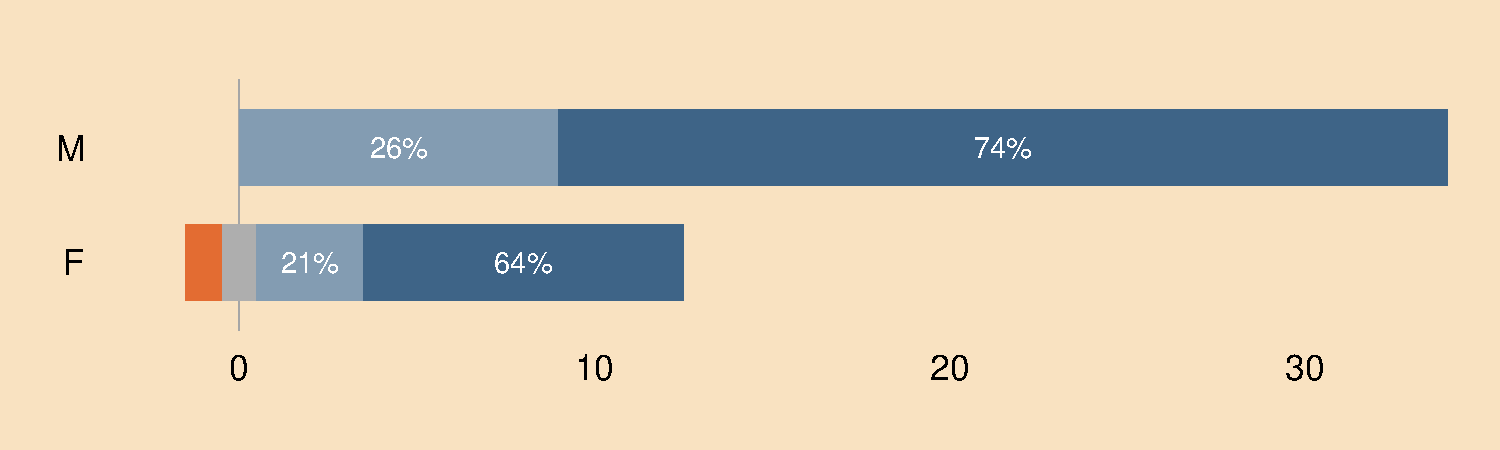
\includegraphics[align=t,trim={0 5mm 0 15mm},clip,width=10cm]{fig/culture/paolo8.pdf}\\
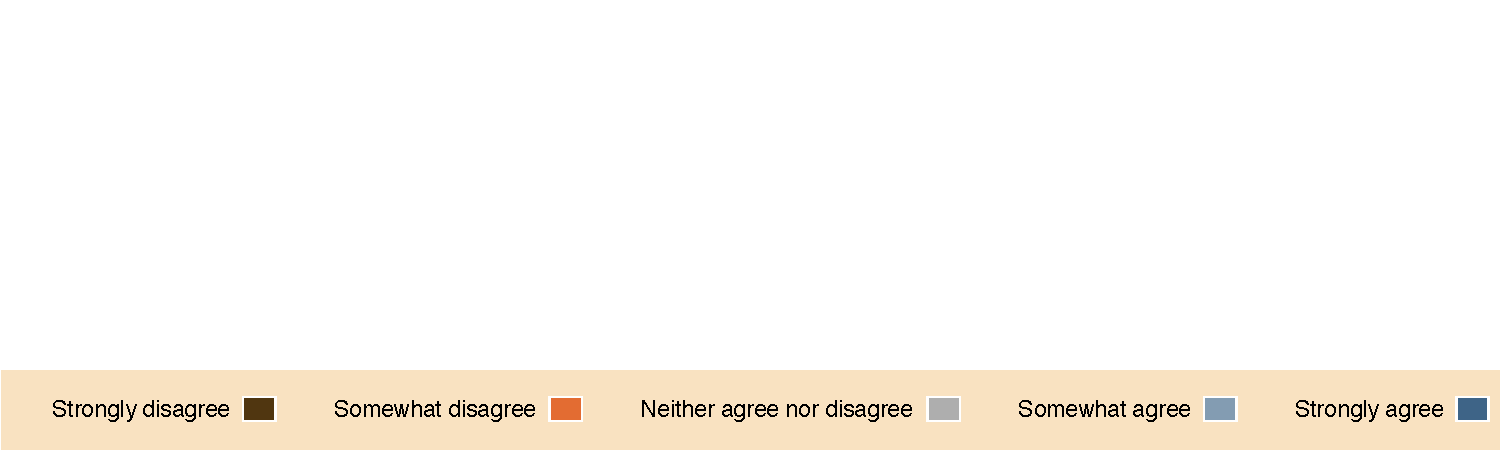
\includegraphics[trim={6mm 0 0 0},clip,width=14.5cm]{fig/legend5col.pdf}
\end{figbox}

\pagebreak 
\subsubsection*{Actions and Priorities}
All actions proposed by the School of Computer Science and Information Technology (CSIT) are presented as follows:

\newtcbtheorem{TEMPaction}{\textsf{ACTION 2.2.1:   Recruitment and Unconscious Bias Training for Research Positions}}{%
        theorem name,%
        separator sign={ },
        borderline west={3pt}{0pt}{RoyalBlue},
        colback=titlebglight!30!white,
        colframe=titlebglight!30!white,
        coltitle=titlebgdark,
        sharp corners,
        left=2mm,
        top=2mm,
        bottom=1mm,
        right=1mm,
        enhanced,
        arc=0pt,
        outer arc=0pt,
        enhanced,
        fonttitle=\sffamily\bfseries\footnotesize,
        fontupper=\sffamily,
        boxrule=0mm,   
        after skip=20pt plus 2pt
    }%
    {TEMPaction}
    
\begin{TEMPaction}{}{}
\actrecruitmenttraining
\hfill{
    \hypersetup{hidelinks}
    \hyperlink{c7}{\gotoactionsymbol{}}
}
\end{TEMPaction}

Actions are numbered in the same way as figures and tables, explained above. The action number is followed by an action title, which is indexed in the List of Actions on Page~\pageref{listofactions}.



The \gotoactionsymbol{} icon is a hyperlink that provides quick access to the Actions table in Section~3. To go back to where the action is introduced, a hyperlink is provided in the Actions table.

On occasion, reference is made to Actions proposed by the university in its institutional Athena Swan Bronze Award Action Plan. These are presented as follows:

\begin{UCCaction}{5.1.3}{}\hypertarget{act513}
Establish a promotion pathway to Professor Scale 1, drawing on learnings for gender equality implemented in schemes for promotion to SL (Jan 2019) and Prof Scale 2 (Oct 2019) scheme calls (see Action 5.1.4).
\end{UCCaction}

Priorities as set out in Section 2.5 are presented as follows:

\begin{priority}{5}
Promote a culture of inclusivity and belonging.
\hfill{
    \hypersetup{hidelinks}
    \hyperlink{p5}{\gotoactionsymbol{}}
}
\end{priority}

The \gotoactionsymbol{} icon is a hyperlink that provides quick access to the appropriate part of the Actions table in Section~3, listing all actions relevant to that particular Priority.

\endgroup 

%TC:endignore 

%% no margin in tables except on front page
\setlength\tabcolsep{0pt} 



%% Table of contents; only print chapters and sections
\setcounter{tocdepth}{1}
\tableofcontents

%TC:endignore

%%%%%%%%%%%%%%%%%%%%%%%%%%%%%%%%%%%%%%%%%%%%%%%%%%%%%%%%%%%%%%%%%%
%% Main file for meta stuff; actual contents starts 
%% in 'body.tex' as top-level main file.
%% Prefixing names with _ and __ to ensure they're 
%% sorted at the top of the file list, in case you were wondering.

%% This file includes individual chapters only. 
%% Chapter files may or may not be further divided 
%% into smaller chunks (e.g. sections), but they are 
%% not handled here. Chapter files are dealt with here, only.

%TC:ignore
\listoffigures
\listoftables 



{
  \sffamily 
  %%% Bit of a HACK to get the page numbers also in \sffamily: set the default font to \sffamily, and restore to \rmdefault.
  %%% But seemingly not other easy way that doesns't take a day to figure out.
  \renewcommand\familydefault{\sfdefault}
  \tcblistof[\chapter*]{thm}{List of Actions}\label{listofactions}
 %% \tcblistof[\chapter*]{lis}{List of Listings}
  \renewcommand\familydefault{\rmdefault}
}
\addcontentsline{toc}{chapter}{List of Actions}

%% Ensure the TOC contains the right page number for Terms & Abbreviations.
\cleardoublepage
\phantomsection
\addcontentsline{toc}{chapter}{List of Terms and Abbreviations}
{
  \footnotesize 
  \printacronyms[include=A,name=List of Terms and Abbreviations]
}



\mainmatter

%% Do NOT set these before the main page is made, because logos don't get aligned.
\widowpenalty10000
\clubpenalty10000
%TC:endignore


%
%


\chapter[An introduction to the department's Athena Swan work]{An introduction to the department's\\Athena Swan work}\label{chap:intro}

\vspace*{-1cm}

\instr{In Section 1, applicants should evidence how they meet Criterion A:
\begin{itemize}
\item Structures and processes underpin and recognise gender equality work and, where relevant, wider equality work 
\end{itemize}
Recommended word count: 2000 words
}


\section{Letter of Endorsement from the Head of School}

\instr{
Insert (with appropriate letterhead) a signed letter of endorsement from the head of the department. The letter should comment on:
\begin{itemize}
    \item the link between the Athena Swan Ireland principles and the department's strategy; \item leadership of the head of department in advancing equality, including any involvement in the self-assessment or specific actions; 
    \item evidence of how the department's equality work is led and supported by the department's senior management;
    \item key priorities, achievements and challenges relating to gender equality as discerned from the self-assessment; 
    \item where relevant, key priorities, achievements and challenges relating to additional equality grounds, as discerned from the self-assessment; 
    \item priority actions to address the issues and opportunities identified.
\end{itemize}

}


\begin{mdframed}[backgroundcolor=white,                
                linecolor=black,
                innerleftmargin=1.5cm,
                innerrightmargin=1.5cm,
                innertopmargin=1cm,
                innerbottommargin=1cm,
                usetwoside=false,
                splitbottomskip=2cm,
                splittopskip=2cm,
                everyline=true                
                ]


\sffamily 
\footnotesize

\includegraphics[width=4cm,right]{img/ucclogo.png}\\[.1in]
\begin{tabular}{ll}
\begin{minipage}{8cm}
%TC:ignore
Dr Sara Fink\\
Head of Athena SWAN Ireland\\
Advance HE\\
First Floor, Napier House\\
High Holborn\\
London WC1V 6 AZ\\
United Kingdom\\
%TC:endignore
\end{minipage}
&
\begin{minipage}{4cm}
\tiny  
%TC:ignore
Professor Utz Roedig\\
School of Computer Science and\\Information Technology\\
University College Cork\\
Western Gateway Building\\
Western Road, Cork, Ireland\\
u.roedig@ucc.ie\\
+353 21 420 5900\\
%TC:endignore
\end{minipage}\\
\end{tabular}


30 November, 2022\\[.1in]
Subject: \textbf{Endorsement of Athena SWAN Bronze Award Application}\\[.1in]

Dear Dr Fink,\\

As Head of School of Computer Science and Information Technology (CSIT), I wish to commit my full support to the Athena Swan (AS) Ireland Principles and pledge to imbed these principles into the culture, policies, and practices of the school. In addition to forming an Equality, Diversity, and Inclusivity (EDI) Implementation Committee (EDIIC), each School standing committee will have an Athena Swan Champion; this process will align with the allocation of all school administrative duties.

CSIT is one of the largest schools in the College of Science, Engineering and Food Science (SEFS).  It is a multifaceted ecosystem, composed of academics (33, 9\% female), professional, managerial and support staff (25, 48\% female), research staff (23, 17\% female), postgraduate research (45, 13\% female), postgraduate taught (129, 46\% female) and undergraduate (390, 24\% female) students. 

Traditionally, Computer Science is a male dominated discipline; our flagship undergraduate programme is 14\% female.  Recognising this, we previously formed partnerships with Psychology and Digital Humanities and developed two interdisciplinary undergraduate degrees.  These have been strategically important initiatives which have increased our female undergraduate numbers (24\%). Two female academic staff members have been appointed to teach on, support and develop the gender balance of these programmes. 

We started our AS self-assessment in Spring 2021.  As Head of School, I appointed Professor John Morrison as Chair of the Self-Assessment Team (SAT). Appointing a senior experienced leader as Chair of the SAT demonstrates my commitment supporting the adoption of the AS Principles in the school.  The SAT was composed of 29 school members, 41\% female.  

The SAT has identified five priority areas that will be addressed over the next four years. 

\begin{enumerate}

\item Firstly, we need to develop governance structures, policies and procedures to ensure that the Athena Swan Ireland Principles are embedded in the school.  I will address this priority through the establishment of an EDI Implementation Committee, appointing a Chair from senior staff.  The committee will have the authority to oversee and implement the action plan. 

\item Currently, there is a dearth of female academic (9\%) and research (17\%) staff particularly at higher grades.  Increasing the ratio of female applicants for staff posts in these cohorts is expected to improve the staff gender balance.  I will prioritise the development of guidelines to improve the school's gender imagery and advertising, and actively target females encouraging them to apply for academic and research positions whilst providing focused support for female staff in the school. 

\item Our aim to increase the number of female students registered in undergraduate and postgraduate programmes will continue through ongoing partnerships with our colleagues in digital humanities and psychology. By understanding our current student's motivation to study Computer Science allows us to develop strategies to improve gender balance in our core CS programmes.  We plan to provide a richer experience for our current female students through internships and scholarship, thus providing female role models for future students. 

\item In 2023, I will restart the Performance Development and Review Process (PDRS) to improve support for staff development and career progression.  Mentors will be appointed to female staff and training, and funding workshops will be arranged to enhance their change of promotion.  

\item I am committed to promoting a culture of inclusivity and belonging in the school, and will create a policy defining how the school will implement statutory family leave. I will ensure that students from diverse backgrounds have opportunities to study with us.  We will keep in touch with colleagues from other schools, for example through the \ac{TLCF}, to ensure that we are in line with the EDI agenda both nationally and internationally.

\end{enumerate}

To ensure that our actions are having a positive impact and desired effect on the EDI culture, we will conduct a review towards the end of 2026 to evaluate progress and staff and student satisfaction and experience. 

The information presented in the application is an honest, accurate and true representation of the school. 



Yours sincerely,


\includegraphics[width=1in]{img/signature-roedig.png}

Utz Roedig\\
Professor of Computer Science\\
Head of School of Computer Science and Information Technology

\end{mdframed}



%TC:ignore
\subsubsection{Confirmation}
\textcolor{titlebgdark}{
The information presented in the application (including qualitative and quantitative data) is an honest, accurate and true representation of the department. {\hfill \LARGE \XBox }
}
%TC:endignore

% \begin{labelboxcode}{hello}{Hello world}
% Test 1
% \end{labelboxcode}

\clearpage 
\section{Governance and recognition of equality, diversity and inclusion work}

\subsection{Provide a description of the department's structures to advance equality. This should include:}
\instr{
\begin{itemize}
\item	information on where the department is in the Athena Swan process; 
\item	an organigram of the department's key management and/or committee structures, with headcount by gender, that includes the formal reporting structures in place to carry out and support Athena Swan activity and, if applicable, wider EDI work;
\item	information on the relationship of department structures with departmental Athena Swan structures and, if applicable, EDI structures, including mechanisms for sharing the findings of self-assessment as well as good practice;
\item	information on support provided by the department for the application;  
\item	information on formal processes in place to resource, distribute, recognise and reward Athena Swan and, where applicable, EDI work, referencing department-level policies where appropriate;
\item	resource provision for the action plan and associated activities to ensure effective implementation;
\item	any other relevant structure and organisation information, such as the department's relationship with community partners;
\item	confirmation that staff and students are recorded as the gender with which they identity in this submission.
\end{itemize}
}


\subsubsection{Information on where the department is in the Athena Swan process}

In response to a call for expressions of interest, the school of \ac{CSIT} appointed an \ac{AS} Champion in 2019 in recognition of the importance of the \ac{EDI} agenda at university level, to increase awareness and to set the groundwork to prepare for an AS Bronze application.  Between 2019 and 2022, the Champion represented the school at the College of \ac{SEFS}, and provided regular updates at school meetings. 

A \ac{SAT} was set up in Spring 2021 and all school members were invited to join; the final composition ensured gender representation and role equality among staff and postgraduate students (see Table~\ref{tab:initialexpandedsat}, Page~\pageref{tab:initialexpandedsat}). 

This application reports on three years of data, namely from 2017-2020. 
Data cited in this application have been gathered from a staff survey conducted by the university's \ac{EDI} unit in June-July 2021, and three focus group sessions in May-June 2022. Data maintained as part of local CSIT records are also cited to supplement centralised records. 



\subsubsection{An organigram of the department's key management and/or committee structures, with headcount by gender, that includes the formal reporting structures in place to carry out and support Athena Swan activity and, if applicable, wider EDI work}


Table~\ref{tab:keyroles} summarises leadership roles
within the school, reflecting a dearth of women in senior academic and research grades. 
The term ``Research Director'' in Table~\ref{tab:keyroles} refers to senior
director-level roles in one of the multi-institutional national research centres funded by \ac{SFI} that the school is involved in (Table~\ref{tab:researchcentres}), and two Centres for Research Training (CRT) for training PhD students, also funded by SFI (Table~\ref{tab:crts}). 



\begin{tabbox}{!th}

\caption{Key roles within CSIT by gender}
\label{tab:keyroles}
\footnotesize 

\sisetup{
    group-digits=all,
    group-minimum-digits=4,
    table-format=2.1,
    mode=text,
    reset-text-series = false, 
    text-series-to-math = true,
    reset-text-family=false, 
    text-family-to-math=true
}
\begin{tabular}{p{4cm}
                S[table-format=2.1]
                !{\quad}
                S[table-format=2.1] 
                p{3cm} 
                p{4cm} 
                S[table-format=2.1]
                !{\quad}
                S[table-format=2.0] 
                }
\toprule 
\multicolumn{3}{c}{\textmd{School Leadership}} %JPM Changed Academic to School
&&
\multicolumn{3}{c}{\textmd{Research Leadership}}\\ 
\cmidrule{1-3}\cmidrule{5-7}
& {F} & {M} & & & {F} & {M} \\ 
\midrule 
Head  of School  & 0 & 1 && Research Directors\interdis & 0 & 4\\ %JPM Changed Directors to Research Directors
\cdashline{1-3}\cdashline{5-7}
PMS Managers & 1 & 1& & Principal Investigators & 0& 10\\
\cdashline{1-3}\cdashline{5-7}
%AOD, GP, GR, IP, AZ, MvD, KJS, DM
Programme Directors & 2 & 6 & & SFI Funded Investigators\interdis\interdis & 1& 8\\
\cdashline{1-3}
Committee Chairs& 0 & 8 &&&&\\
\bottomrule 
\end{tabular}
\begingroup
\sffamily 
\singlespacing 
\interdis{} Director refers to Directors or Co-Directors of SFI Research Centres.\\
\interdis\interdis{} SFI Funded Investigator (FI) is a role within an SFI Research Centre, such as Connect and Lero; an FI leads one or more research projects within such a centre, and must be approved by SFI.
\endgroup 

\end{tabbox}

\begin{figbox}{!t}
    \caption{Overall school management and committee structures / programme directors}
    \label{fig:schoolstructure}    
    \centering 
    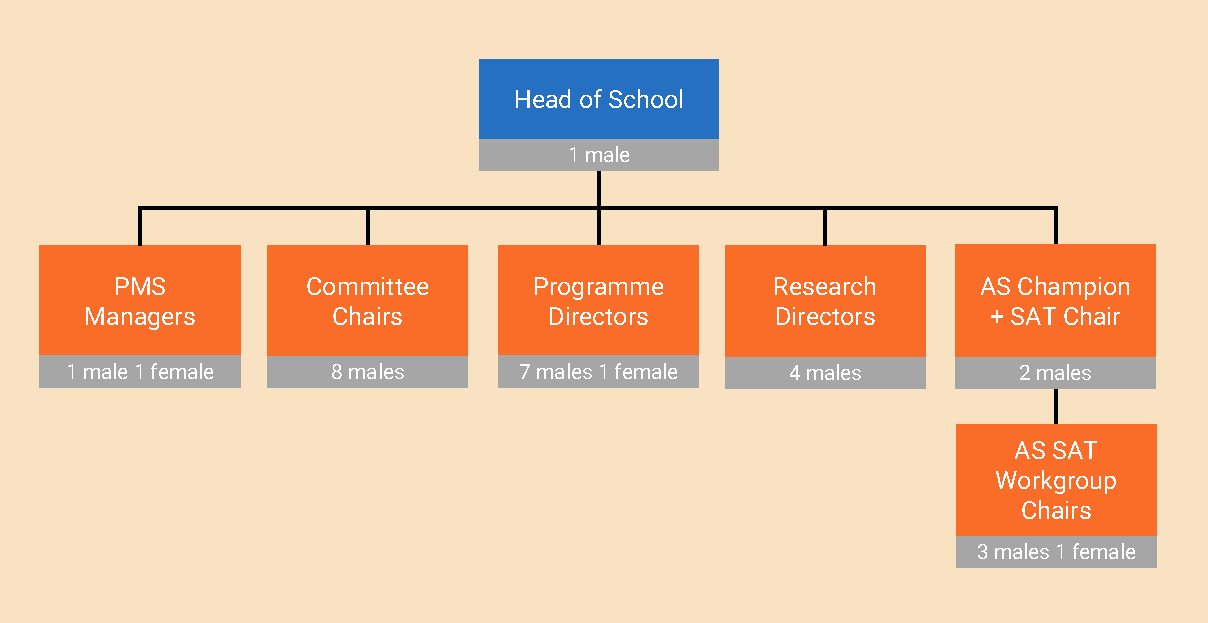
\includegraphics[trim={5mm 5mm 5mm 5mm},clip,width=12cm]{fig/schoolmanagamentdec21.pdf}
\end{figbox}

Figure~\ref{fig:schoolstructure} shows the gender distribution in school leadership roles. Most  staff have administrative responsibilities and serve in school committees.  Key academic administrative responsibilities in the school are clearly gender imbalanced. The greatest gender imbalance is in academic staff, particularly at senior level (Figure~\ref{fig:schoolstaff}).



\begin{figbox}{!ht}
    \caption{School staff at CSIT per Autumn 2022}
    \label{fig:schoolstaff}
    \centering    
    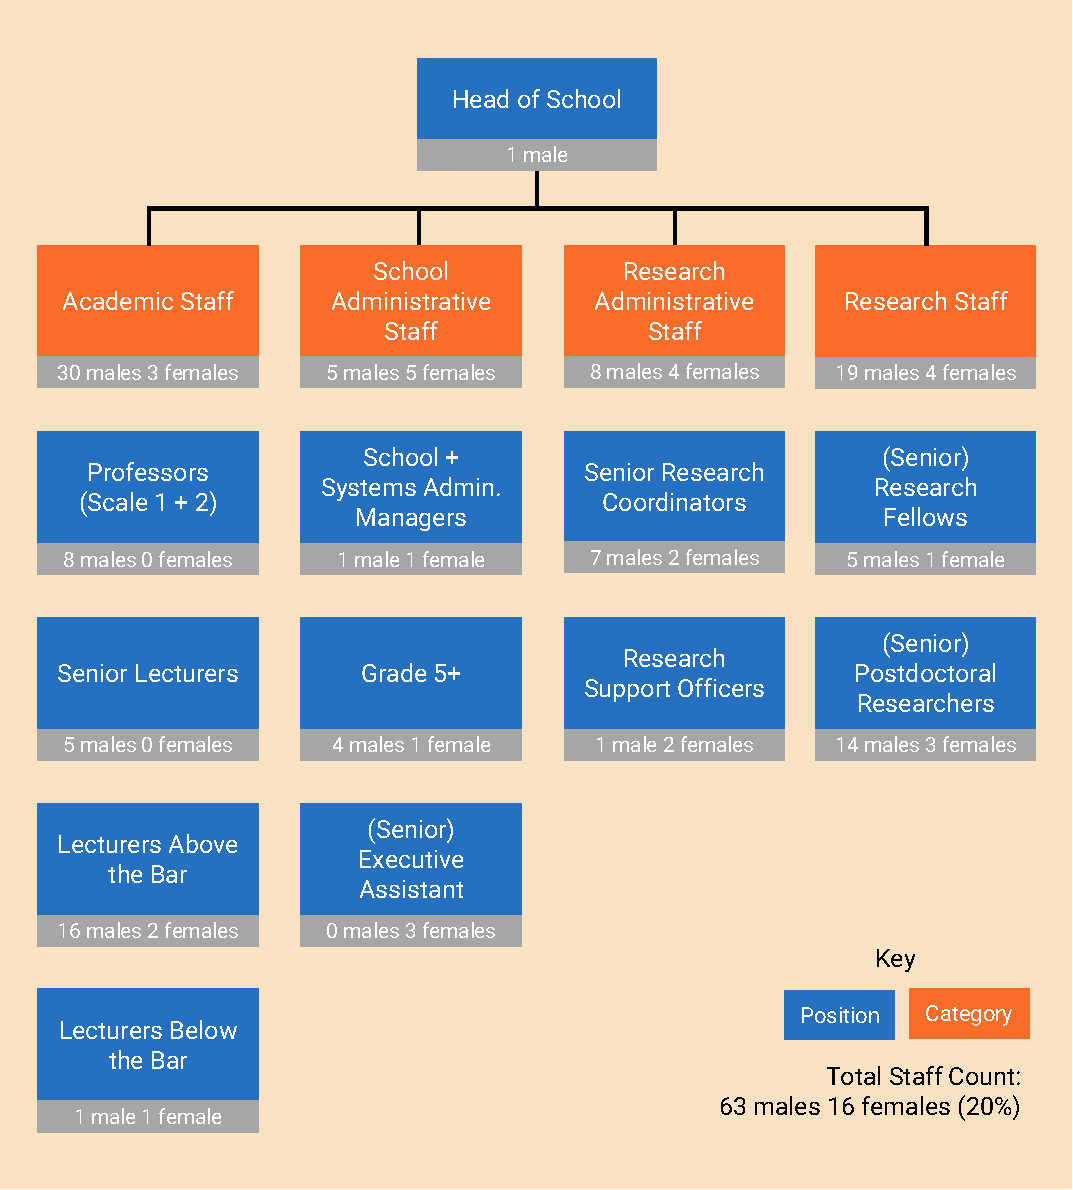
\includegraphics[trim={5mm 5mm 5mm 5mm},clip,width=12cm]{fig/neworganigramDec21.pdf}\\
    {\sffamily\footnotesize \RaggedRight Note: numbers per Autumn 2022; some may differ in other figures and tables.}
\end{figbox}






The school has eight committees to support school activities. 
Table~\ref{tab:gender:committees} shows 
the gender distribution of committee members. 



\begin{tabbox}[11cm]{!th}
\caption{Gender representation in School committees}
\label{tab:gender:committees}
\sisetup{
    group-digits=all,
    group-minimum-digits=4,
    group-separator = {,},
    table-format=4.1,
    mode=text,
    reset-text-series = false, 
    text-series-to-math = true,
    reset-text-family = false, 
    text-family-to-math = true
}
\footnotesize   
\begin{tabular}{p{6cm} 
                !{\quad}
                S[table-format=2.0]
                !{\quad}
                S[table-format=2.0]
                !{\quad}
                S[table-format=2.0\%]
                !{\quad}
                S[table-format=2.0]
                }

\toprule 
Role & {Male} & {Female} & {Female \%} & {Total}\\
\midrule 
Committee Chairs & 8 & 0 & 0\% & 8\\
\hdashline
Committee Members & 16 & 7 & 30\% & 23 \\
\hdashline
All Committee (Chairs and Members) & 24 & 7 & 23\% &31\\
\bottomrule 
\end{tabular}


\end{tabbox}




\subsubsection{Information on the relationship of department structures with departmental Athena Swan structures and, if applicable, EDI structures, including mechanisms for sharing the findings of self-assessment as well as good practice}

The SAT engaged intensively with the university's EDI unit and other schools within the university seeking \ac{AS} accreditation. It also consulted with colleagues in cognate schools from other universities that had already successfully engaged with the AS process. The SAT Chair regularly reported progress through a standing item on the school's monthly meeting agenda.



\subsubsection{Information on support provided by the department for the application}
The school provided full administrative support to the SAT in organising
meetings and taking minutes. The School Manager coordinated the
collection of local data with with the Research Centre administrators
and  compiled this data into a suitable format for the SAT to review.
The \ac{HOS} actively promoted the SAT activities at all school meetings,
encouraging staff to take part in discussions and giving adequate
time for everyone to comment on the process and findings.
In addition, the university provided extensive support to the school during the production of this application. The EDI unit supported in the production, administration and collation of results of the staff survey. In addition, Academic Support Services and HR provided data. Although not required for this application, the university also makes funds available for practical support for AS applications.   


\subsubsection{Information on formal processes in place to resource, distribute, recognise and reward Athena Swan and, where applicable, EDI work, referencing department-level policies where appropriate}

The school recently embarked on its AS journey, so apart from the SAT activities, there are currently no formal processes in place to  resource, distribute, or reward AS work.
At the school level, AS activities are recognised by the \ac{HOS} in assigning administrative workload. On appointment, the Chair was relieved of other administrative obligations to concentrate on coordinating the school's AS activities. 


\subsubsection{Resource provision for the action plan and associated activities to ensure effective implementation}

The school has availed of resources provided by the university's EDI unit for the application, including regular feedback and advice from the university's \ac{AS} Project Officer. It will continue to avail of all centrally available resources to support the implementation of CSIT's Action Plan. The \ac{EDIIC} will report any resource deficits to the \ac{HOS} and to the College's AS Steering Committee.
Appropriate changes to the school structures will seek to support the implementation of the action plan (Actions~\ref{action:intro:edi} and \ref{action:intro:agenda}, Page \pageref{action:intro:edi}),  improving the EDI culture.


\subsubsection{Any other relevant structure and organisation information, such as the department’s relationship with community partners}

Since the school embarked on its AS journey, it has been an active member of the university EDI activities and will benefit from, and contribute to, developing best practice.


\subsubsection{Confirmation that staff and students are recorded as the gender with which they identity in this submission}

All requests by staff or students to record their gender preference have been acceded to with confirmation by all data holders to record the appropriate gender.  

\clearpage 
\section{The Self-Assessment Process}


\subsection{Provide information on the preparation and delivery of this application by the department. This should include:}
\instr{
\begin{itemize}
\item  a description of the self-assessment team\index{self-assessment team}, including comment on the roles and responsibilities of individuals, and how these were assigned. The gender of SAT members, their professional/student role in the department, and their specific role in the SAT should be noted in a table; 
\item	information on how the chair was appointed and on what supports or resources the institution and/or department has given the chair to lead the self-assessment process; 
\item	comment on whether the self-assessment team is representative of the department, including if there is adequate representation of senior staff. 
\end{itemize}
}


\subsubsection{A description of the self-assessment team, including comment on the roles and responsibilities of individuals, and how these were assigned. The gender of SAT members, their professional/student role in the department, and their specific role in the SAT should be noted in a table}

The initial SAT  was appointed in March 2021 after an open invitation by the \ac{HOS} to all school members.
The initial 10 %11 
members were a self-selecting group at various stages in their professional careers and included representation from both Professional Management and Support Staff (PMSS) and Academic staff (see Tables~\ref{tab:initialexpandedsat}).

\begin{tabbox}{!b}
\footnotesize 
\caption{Initial and expanded SAT: Gender, leadership, and staff category}
\label{tab:initialexpandedsat}


\sisetup{
    group-digits=all,
    group-minimum-digits=4,
    group-separator = {,},
    mode=text,
    reset-text-series = false, 
    text-series-to-math = true,
    reset-text-family = false, 
    text-family-to-math = true
}   
\begin{tabular}{p{7cm}
                S[table-format=1.0]
                !{\qquad}
                S[table-format=1.0]
                !{\qquad}
                S[table-format=3.0\%]
                p{0.6cm}
                S[table-format=2.0]
                !{\qquad}
                S[table-format=2.0]
                !{\qquad}
                S[table-format=2.0\%]
                p{0.3cm}
                S[table-format=3.0\%]}
\toprule 

  & \multicolumn{3}{c}{\makecell{Initial SAT\\April 2021}} && \multicolumn{3}{c}{\makecell{Expanded SAT\\December 2021}} && {\makecell{\% by staff\\ category}}\\
  \cmidrule{2-4}\cmidrule{6-8}
  & {M} & {F} & {\%F} && {M} & {F} & {\%F} & \\
  \midrule 
 
Chair 										    & 1 & 0 & 0\% && 1 & 0 & 0\% && {n/a} \\
\hdashline
Workgroup Chairs & 0 & 0 & 0\% && 3 & 1 & 25\% && {n/a}\\
\midrule 
Academic									    & 3 & 2 & 40\% && 12 & 3 & 20\% &&52\% \\
\hdashline
Professional Management and Support Staff & 1 & 4 & 80\% && 3 & 6 & 67\% && 31\%\\
\hdashline
Research staff 								    & 0 & 0 & 0\% &&  2 & 3 & 60\% && 17\%\\
\midrule 
Total 										    & 4 & 6 & 60\% && 17 & 12 & 41\% && 100\%\\
  
\bottomrule 
\end{tabular}

\end{tabbox}

\begin{tabbox}{!b}
\caption{Workgroups and distribution of members by gender and staff category}
\label{tab:wgs}
\sisetup{
    group-digits=all,
    group-minimum-digits=4,
    group-separator = {,},
    table-format=4.1,
    mode=text,
    reset-text-series = false, 
    text-series-to-math = true,
    reset-text-family = false, 
    text-family-to-math = true
}
\footnotesize   
\begin{tabular}{p{8cm} 
                !{\quad}
                S[table-format=2.0]
                !{\quad}
                S[table-format=2.0]
                !{\quad}
                S[table-format=2.0]
                !{\quad}
                S[table-format=2.0]
                !{\quad}
                S[table-format=2.0]
                !{\quad}
                S[table-format=2.0]                            
                }

\toprule 
%& {\multicolumn{2}{c}{Gender}} & {Staff category}\\
       
&\multicolumn{2}{c}{\makecell{Gender}} & & \multicolumn{3}{c}{Staff category}\\      
\cmidrule{2-3}\cmidrule{5-7}
Workgroup & {M} & {F} & & {Academic} & {PMSS} & {Research}\\ 
\midrule 
Chair's Workgroup\textsuperscript{1} & 5 & 2 && 6 & 1 & 0\\
\midrule
WG1:  Department and Its Context & 3 & 1 & & 2 & 2 & 0\\
\hdashline
WG2: Academic and Research Careers & 6 & 3 & & 5 & 0 & 4\\
\hdashline
WG3: Professional, Managerial and Support Staff Careers & 3 & 3 & & 2 & 4 & 0\\
\hdashline
WG4: Inclusion and Belonging & 3 & 3 & & 4 & 1 & 1 \\
\hdashline
Administrative support & 0 & 2 & & 0 & 2 & 0\\
\midrule
Total SAT members (29), by gender, and category\textsuperscript{1} & 17 & 12 && 15 & 9 & 5 \\
\bottomrule 
\end{tabular}
{
\\[2mm]
\sffamily
\textsuperscript{1}Workgroup Chairs are double-counted in the Chair's Workgroup.
}

\end{tabbox}

Midway through the application process, a new Athena Swan Charter was published, including a new application form. 
The SAT responded to these changed by reorganising itself into four thematic Workgroups (WGs) to better match the structure of the new application (see Table~\ref{tab:wgs}). WG Chairs were invited to serve by the SAT Chair, based on their experience in leading teams and knowledge of UCC's institutional structures. WG Chairs were also chosen with the intention of achieving gender balance, although limited by the gender imbalance within the school.

In addition to the four workgroups, a Chair's Workgroup was formed, consisting of the four WG Chairs, the SAT Chair, the School Manager, and the Workgroup Liaison.


Subsequently,  more people were invited 
to join the SAT to maximise representation. This expansion was done by (1) open invitation to all staff, 
and (2) by targeting specific individuals to maximise diversity and promote inclusion. 
The SAT members were at various stages in their career, with many of the senior staff having considerable experience in the running of the school and serving on university committees.
Table~\ref{tab:sat} presents details of all 29 SAT members.\\[.1in]


\clearpage 

%TC:ignore

\newcommand{\mugwidth}{2.7cm}

\begin{mdframed}[backgroundcolor=orangebg,
                 rightline=false,
                 leftline=false,
                 topline=false,
                 bottomline=false,
                 innertopmargin=0pt,
                 ]
\footnotesize                 
\begin{longtable}{P{5cm}
                  !{\qquad}
                  P{\mugwidth}
                  !{\qquad}
                  P{5cm}}
               
\vspace*{-24pt}
\crule{12mm}{3mm}\\[-7mm]

\caption{Athena Swan Self Assessment Team}\label{tab:sat}\\
\toprule
    Name and Position & & Role on SAT\\
\midrule
\endfirsthead
%
\endhead
%
\endfoot
\bottomrule 
\endlastfoot



John Morrison (M) Professor & 
\adjustbox{valign=t}{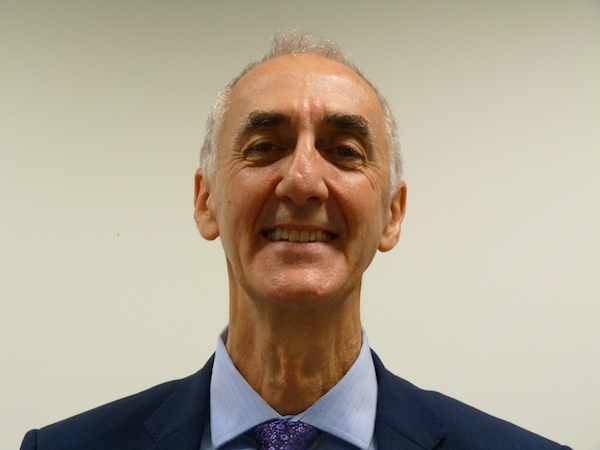
\includegraphics[width=\mugwidth]{img/johnmor.JPG}} & Chair of the CSIT Self-Assessment Team, Member of the Editorial Team \\

\addlinespace
\hdashline

Margaret Hynes (F) Executive Assistant & 
\adjustbox{valign=t}{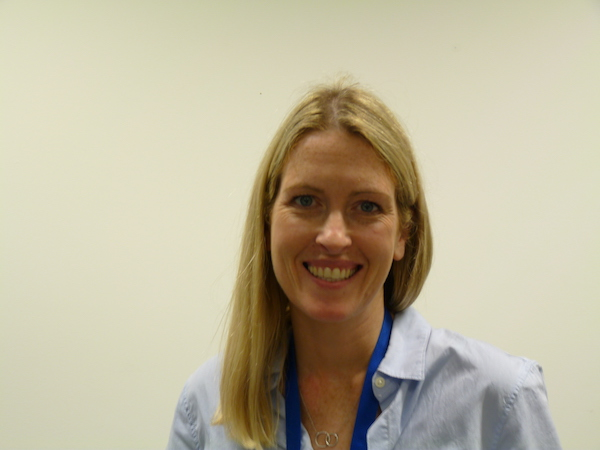
\includegraphics[width=\mugwidth]{img/margaret.JPG}} & SAT Administrative support \\


\addlinespace
\hdashline

Klaas-Jan Stol (M) Lecturer, Funded Investigator at Lero Research Centre, Supervisor at ADVANCE-CRT & 
\adjustbox{valign=t}{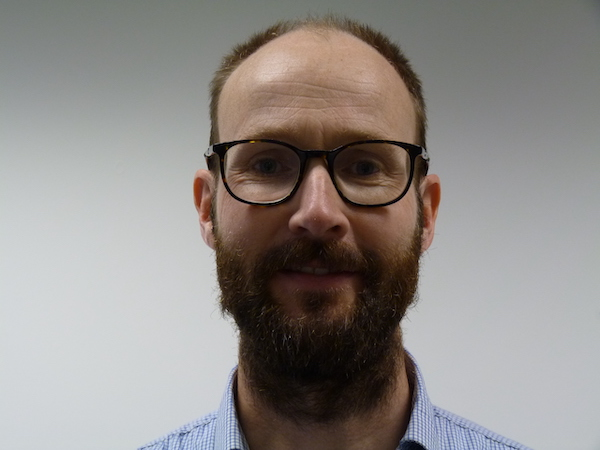
\includegraphics[width=\mugwidth]{img/klaas.JPG}} & Workgroup Liaison; data visualisation, SAT document manager. Member of the Chair's Workgroup, Member of the Editorial Team\\

\addlinespace
\hdashline




Julie Walsh (F) Executive Assistant  & 
\adjustbox{valign=t}{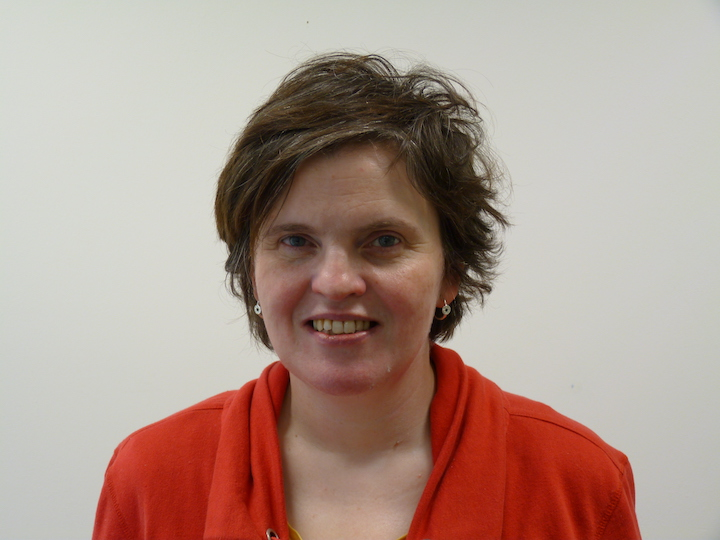
\includegraphics[width=\mugwidth]{img/Julie.JPG}} & SAT Administrative support\\



\addlinespace
\midrule
\multicolumn{3}{c}{Workgroup 1: Department and Its Context }\\
\midrule 

Kieran Herley (M) Lecturer, Chair of the Academic Programmes and Curriculum Development Committee (APCD) & 
\adjustbox{valign=t}{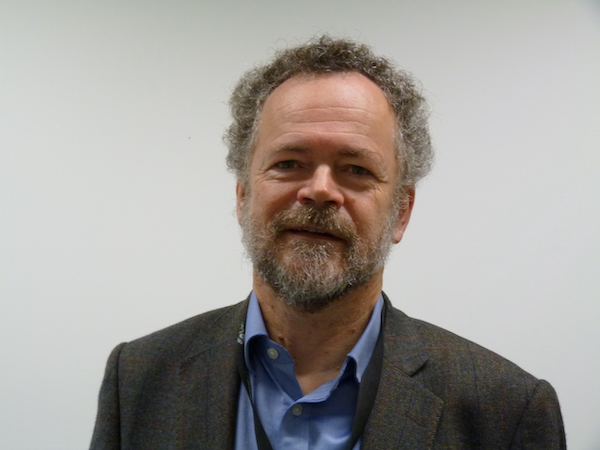
\includegraphics[width=\mugwidth]{img/kieran.JPG}} & Chair of Workgroup 1: Department and Its Context \\

\addlinespace   
\hdashline



Martin Moriarty (M) Systems Administrator &
 \adjustbox{valign=t}{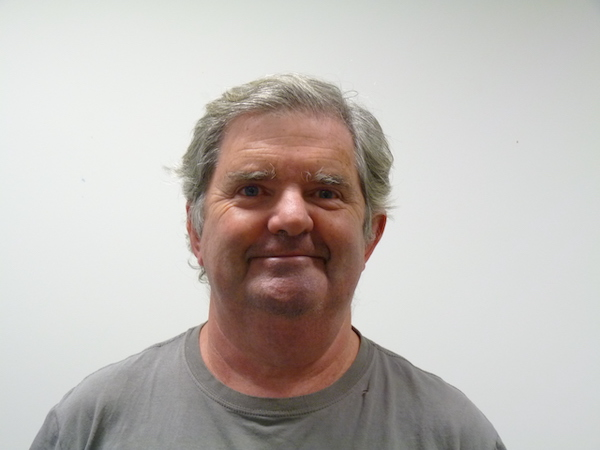
\includegraphics[width=\mugwidth]{img/martin.JPG}} & Member of Workgroup 1: Department and Its Context\\

\addlinespace
\hdashline


John O'Mullane (M) Lecturer &    
\adjustbox{valign=t}{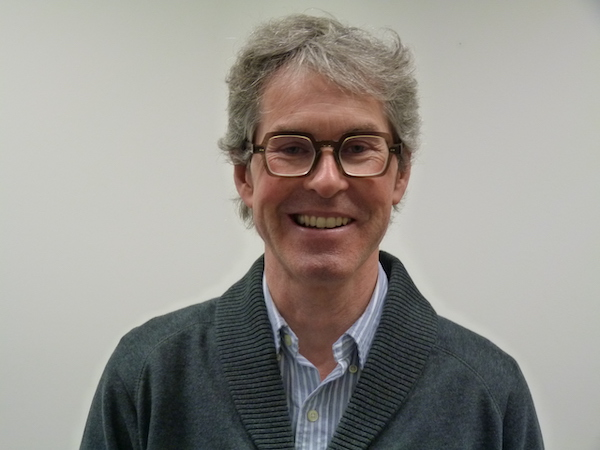
\includegraphics[width=\mugwidth]{img/johnom.JPG}} & Member of Workgroup 1: Department and Its Context \\

\addlinespace 
\hdashline 

Derbhile Timon (F) School Manager &
\adjustbox{valign=t}{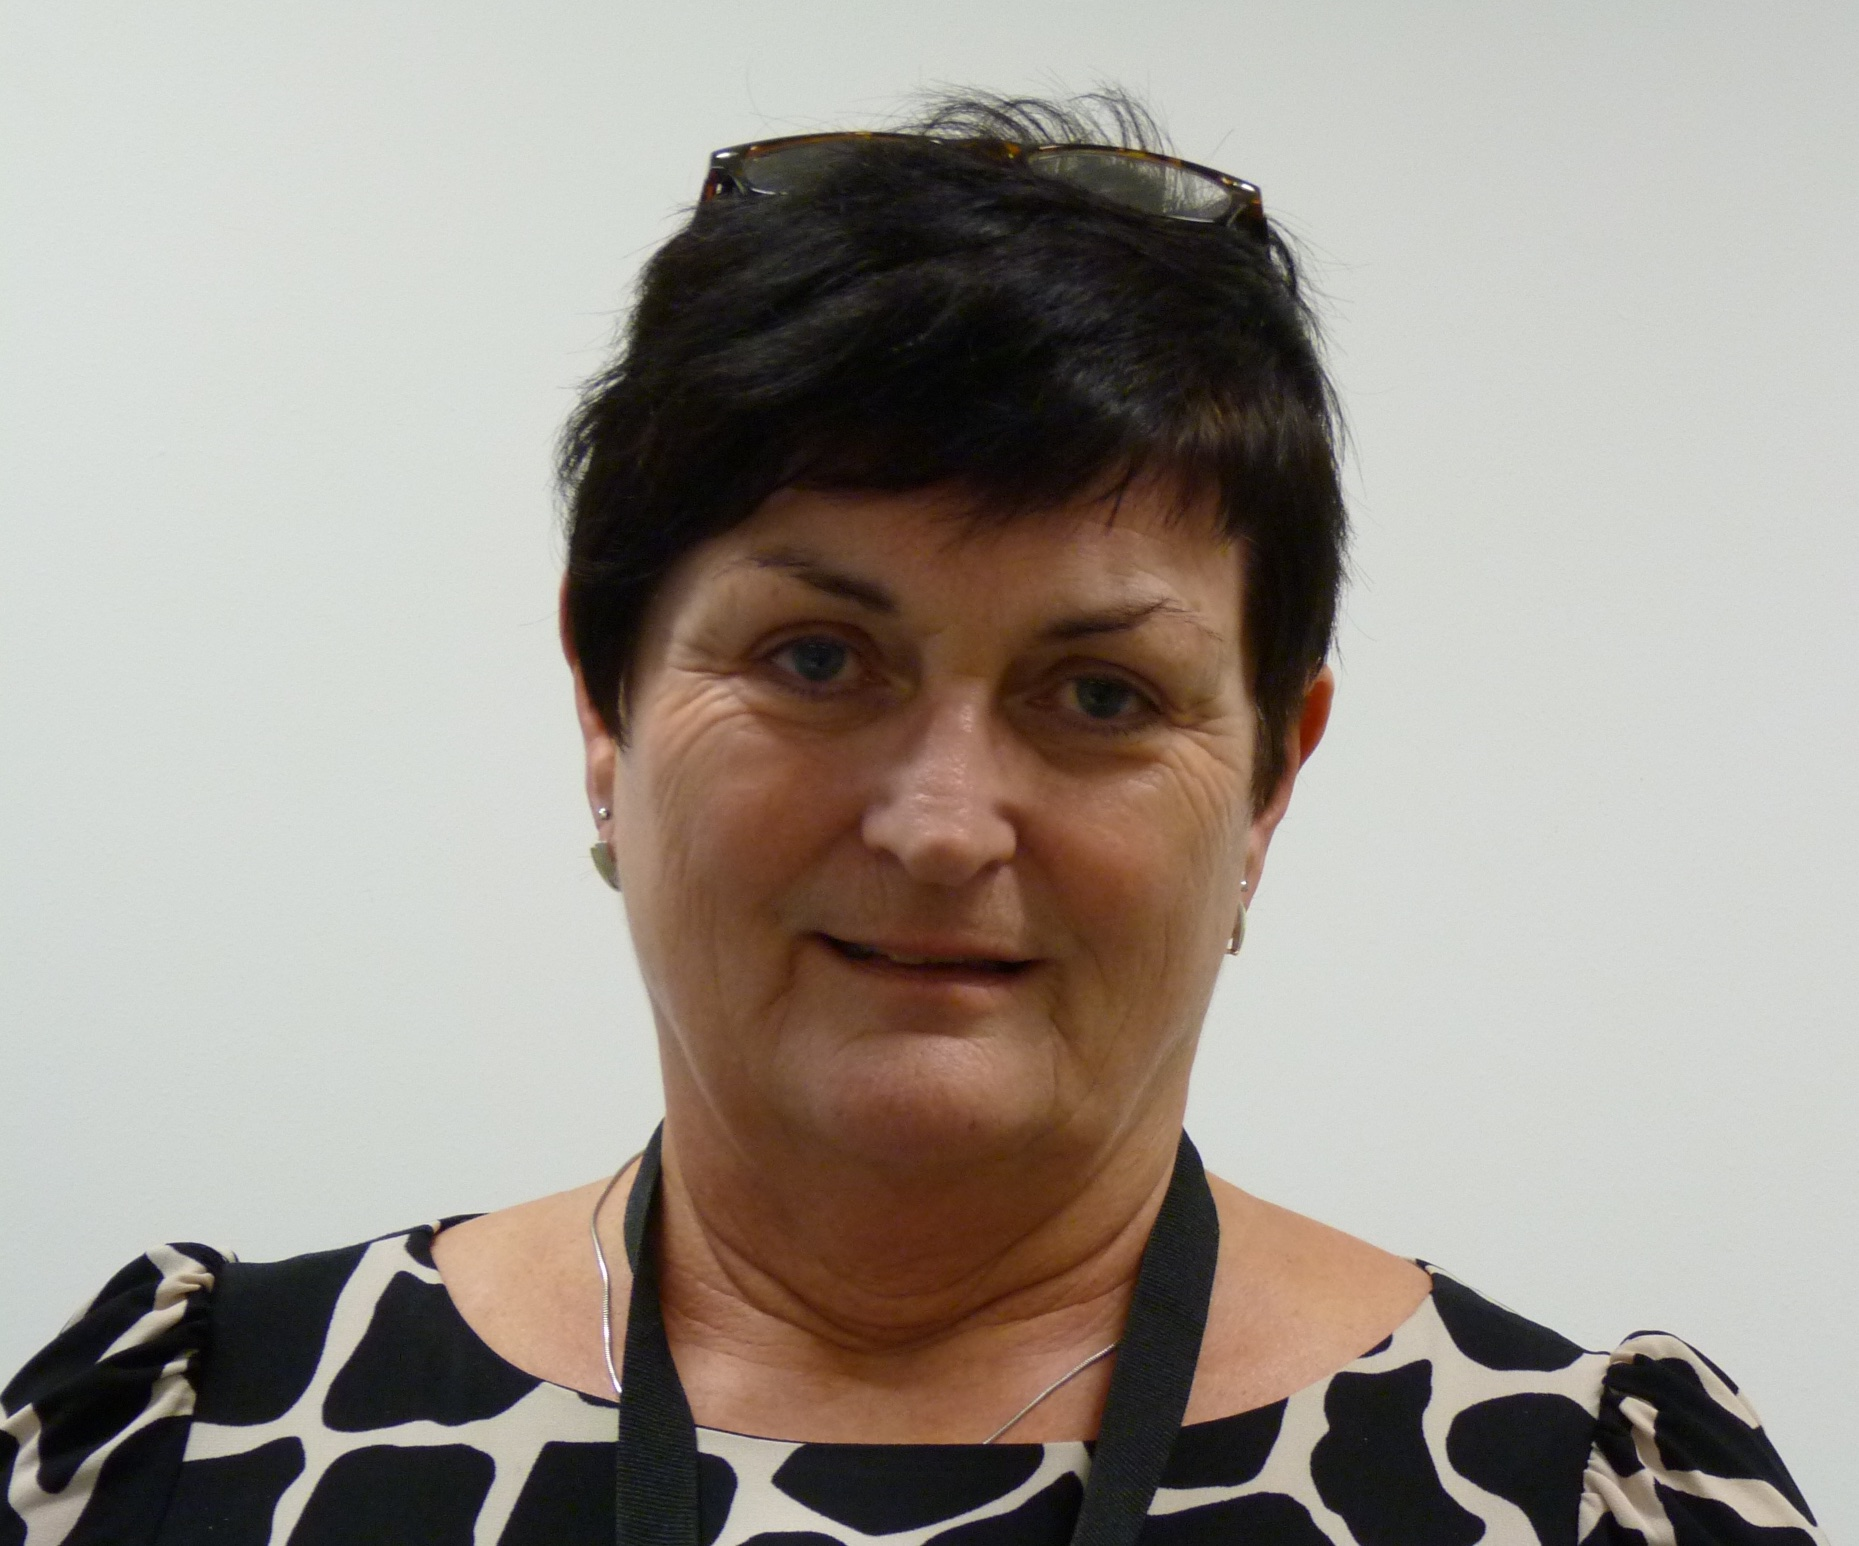
\includegraphics[width=\mugwidth]{img/derbhile.JPG}} & Member of Workgroup 1: Department and Its Context. Member of the Chair's Workgroup, Member of the Editorial Team \\


\addlinespace

\midrule
\multicolumn{3}{c}{Workgroup 2: Academic and Research Careers}\\
\midrule 

Dirk Pesch (M) Professor, Director of ADVANCE-CRT, Co-PI with Connect and Confirm Research Centres; Steering Committee Member of SFI Enable Spoke & \adjustbox{valign=t}{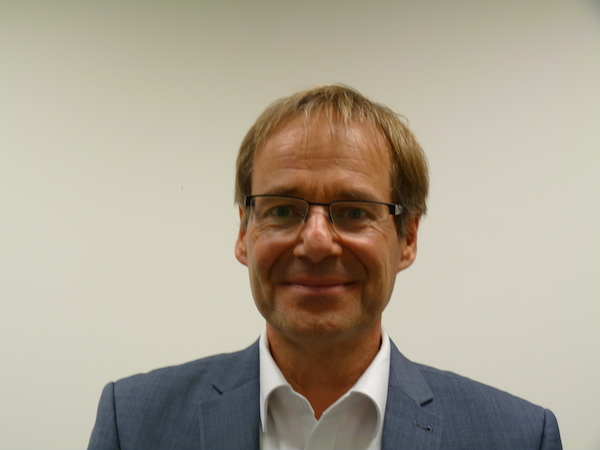
\includegraphics[trim={10mm 0 0 10mm},clip,width=\mugwidth]{img/dirk.JPG}} & Chair of Workgroup 2: Academic and Research Careers. Member of the Chair's Workgroup \\

\addlinespace
\hdashline

Vlad Ionescu (M) PhD Candidate &
\adjustbox{valign=t}{
\includegraphics[width=\mugwidth]{img/vlad.jpg}} & Member of Workgroup 2: Academic and Research Careers\\

\addlinespace
\hdashline

Buvana Ganesh (F) PhD Candidate &
\adjustbox{valign=t}{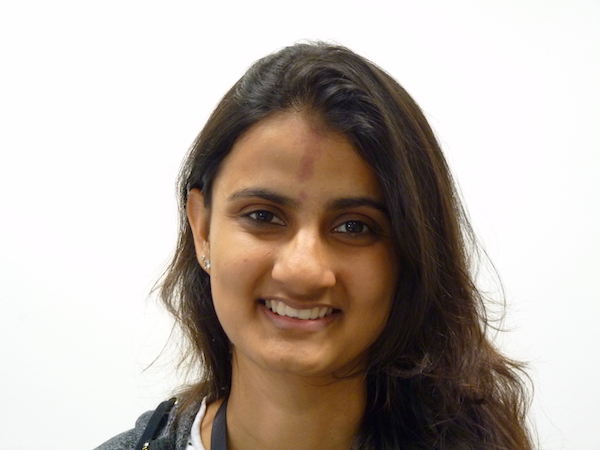
\includegraphics[width=\mugwidth]{img/buvana.JPG}} &Member of Workgroup 2: Academic and Research Careers \\

\addlinespace
\hdashline

Md. Noor-A-Rahim (M) Research Fellow & 
\adjustbox{valign=t}{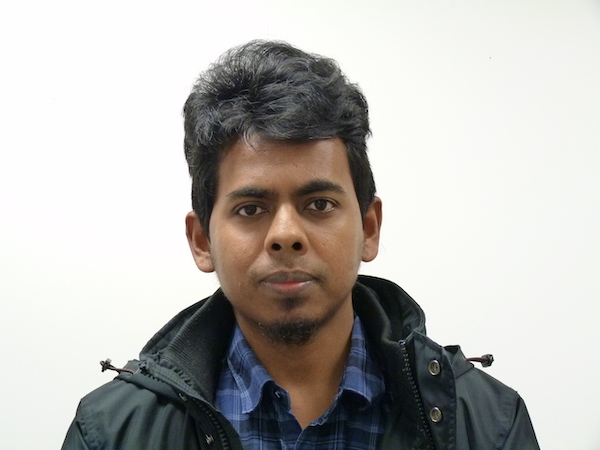
\includegraphics[width=\mugwidth]{img/md.JPG}} & Member of Workgroup 2: Academic and Research Careers \\

\addlinespace
\hdashline

Jason Quinlan (M) Lecturer &
\adjustbox{valign=t}{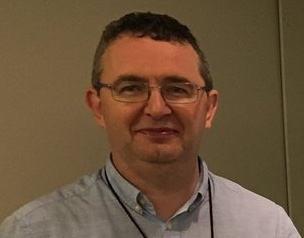
\includegraphics[trim={0 3mm 0 0},clip,width=\mugwidth]{img/jason.JPG}} & Member of Workgroup 2: Academic and Research Careers \\

\addlinespace
\hdashline



Rosane Minghim (F) Lecturer, Supervisor with ADVANCE-CRT & 
\adjustbox{valign=t}{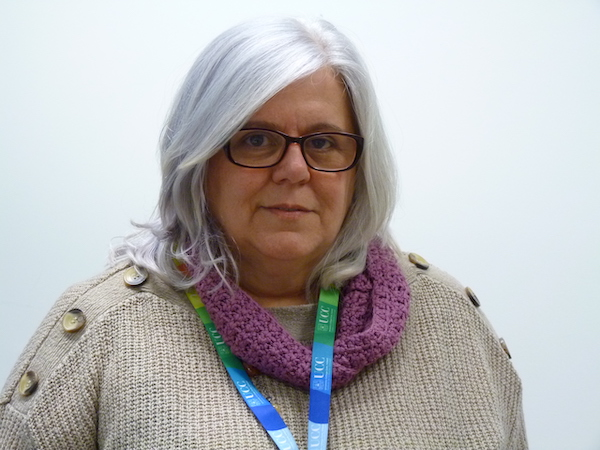
\includegraphics[width=\mugwidth]{img/rosanne.JPG}} & Member of Workgroup 2: Academic and Research Careers\\

\addlinespace
\hdashline


Beg\"{u}m Gen\c{c} (F) Postdoctoral researcher at Insight, now moved to Apple & 
\adjustbox{valign=t}{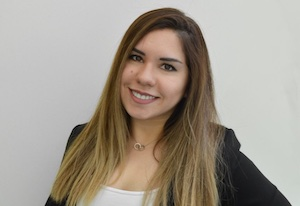
\includegraphics[width=\mugwidth]{img/begum.jpg}} & Member of Workgroup 2: Academic and Research Careers\\

\addlinespace
\hdashline

Barry O'Sullivan (M) Professor, Director of Insight Research Centre, co-PI with Confirm Research Centre &    
\adjustbox{valign=t}{
\includegraphics[trim={0 10mm 0 3mm},clip,width=\mugwidth]{img/barry.JPG}} & Member of Workgroup 2: Academic and Research Careers\\
    
\addlinespace   
\hdashline 

Andrea Visentin (M) Lecturer & 
\adjustbox{valign=t}{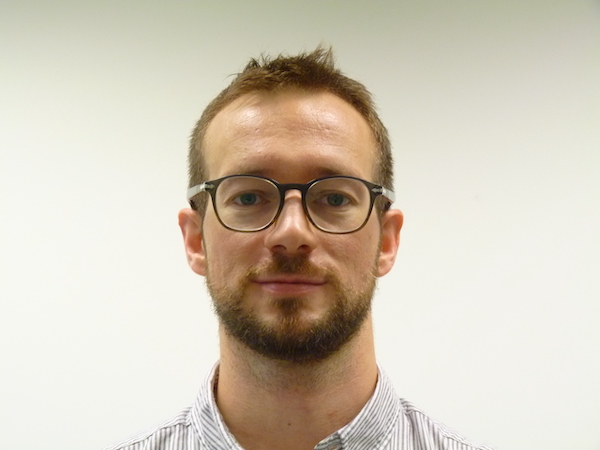
\includegraphics[width=\mugwidth]{img/andrea.JPG}} & Member of Workgroup 2: Academic and Research Careers\\

\addlinespace

\midrule
\multicolumn{3}{c}{Workgroup 3: Professional, Managerial and Support Staff Careers}\\
\midrule 

Aisling O'Driscoll (F) Lecturer, Course Director of BSc Computer Science (BScCS), Funded Investigator at Connect Research Centre, Supervisor at ADVANCE-CRT &
\adjustbox{valign=t}{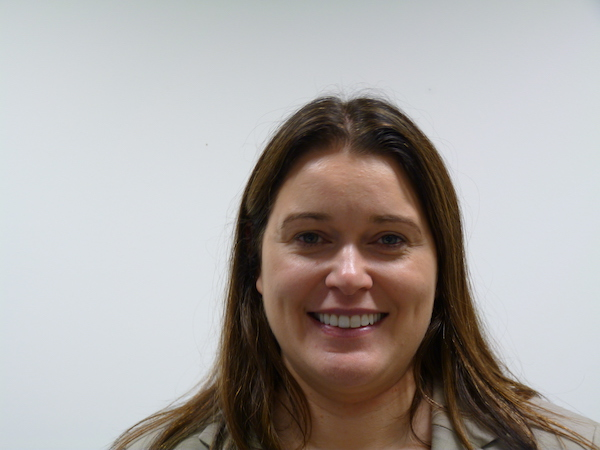
\includegraphics[trim={10mm 0 0 10mm},clip,width=\mugwidth]{img/aisling.JPG}} & Chair Workgroup 3: Professional, Managerial and Support Staff Careers. Member of the Chair's Workgroup\\

\addlinespace
\hdashline

James Duggan (M) Senior Executive Assistant, ADVANCE-CRT &
\adjustbox{valign=t}{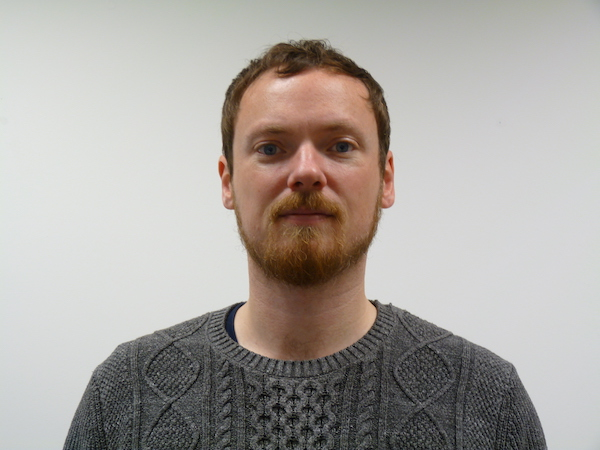
\includegraphics[width=\mugwidth]{img/jamesduggan.JPG}} & Member of Workgroup 3: Professional, Managerial and Support Staff Careers\\

\addlinespace
\hdashline


David O'Byrne (M) Computing Systems Manager & 
\adjustbox{valign=t}{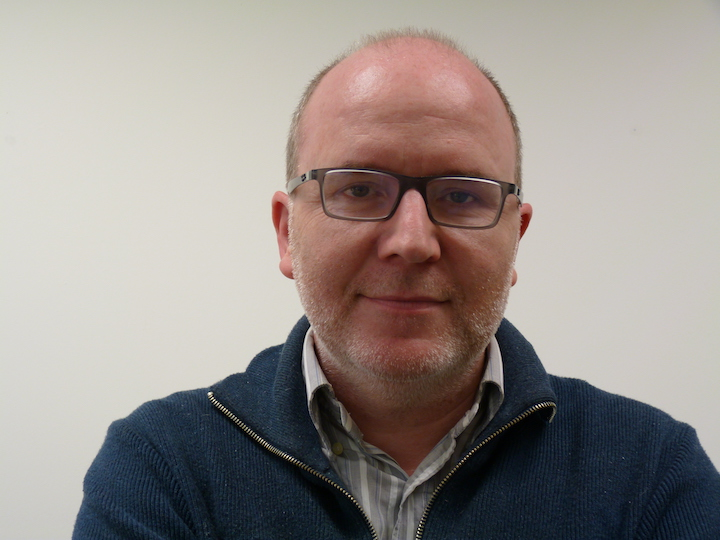
\includegraphics[width=\mugwidth]{img/DavidOB.JPG}} & Member of Workgroup 3: Professional, Managerial and Support Staff Careers \\

\addlinespace    
\hdashline

Adrian O'Riordan (M) Lecturer & 
\adjustbox{valign=t}{
\includegraphics[width=\mugwidth]{img/adrian.jpg}} & Member of Workgroup 3: Professional, Managerial and Support Staff Careers\\
  
\addlinespace
\hdashline

Eleanor O'Riordan (F) Administrator with Insight Research Centre &    
\adjustbox{valign=t}{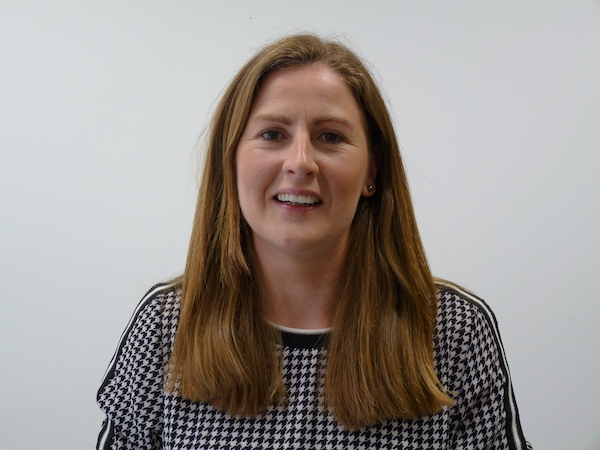
\includegraphics[width=\mugwidth]{img/eleanor.JPG}} & Member of Workgroup 3: Professional, Managerial and Support Staff Careers\\

\addlinespace
\hdashline 


Youngsin O'S\'{e} (F) Senior Executive Assistant  &    
\adjustbox{valign=t}{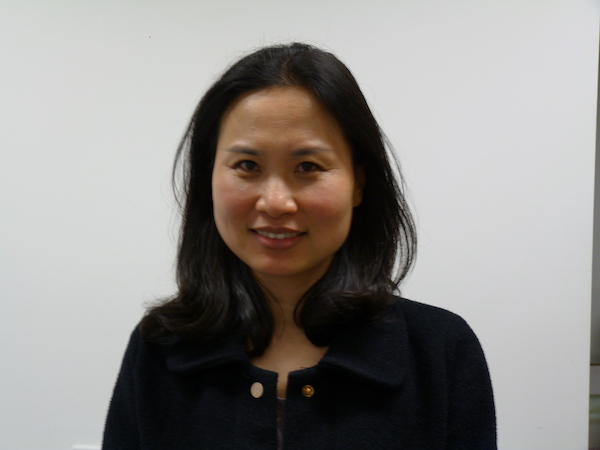
\includegraphics[trim={2mm 2mm 4mm 0},clip,width=\mugwidth]{img/youngsin.JPG}} & Member of Workgroup 3: Professional, Managerial and Support Staff Careers\\

\addlinespace
\pagebreak 
\midrule
\multicolumn{3}{c}{Workgroup 4: Inclusion and Belonging}\\
\midrule 

Paolo Palmieri (M) Lecturer, Funded Investigator at Connect  and Insight Research Centres, Supervisor at ADVANCE-CRT and CRT-AI & 
\adjustbox{valign=t}{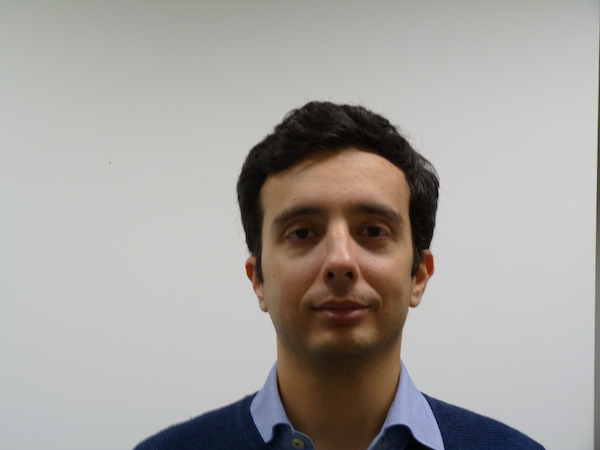
\includegraphics[trim={20mm 0 10mm 16mm},clip,width=\mugwidth]{img/paolo.JPG}} & Chair of Workgroup 4: Inclusion and Belonging. Member of the Chair's Workgroup\\

\addlinespace   
\hdashline 

Andrea Balogh (F) PhD Candidate & %% left low right up
\adjustbox{valign=t}{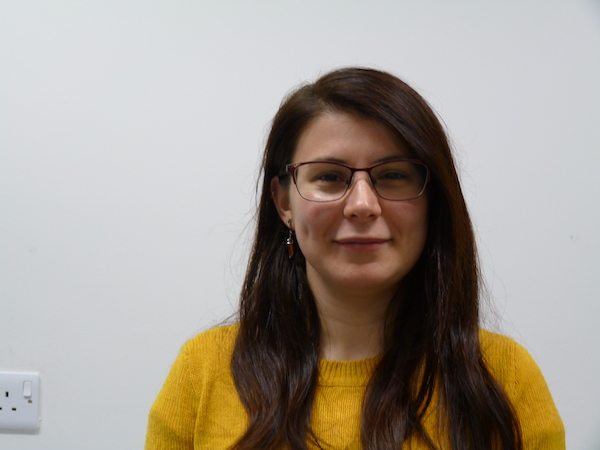
\includegraphics[trim={20mm 10mm 0 10mm},clip,width=\mugwidth]{img/andrea2.JPG}} & Member of Workgroup 4: Inclusion and Belonging\\


\addlinespace
\hdashline


Laura Maye (F) Lecturer, Course Director BA Psychology \& Computing (BAPC), Supervisor with ADVANCE-CRT &
\adjustbox{valign=t}{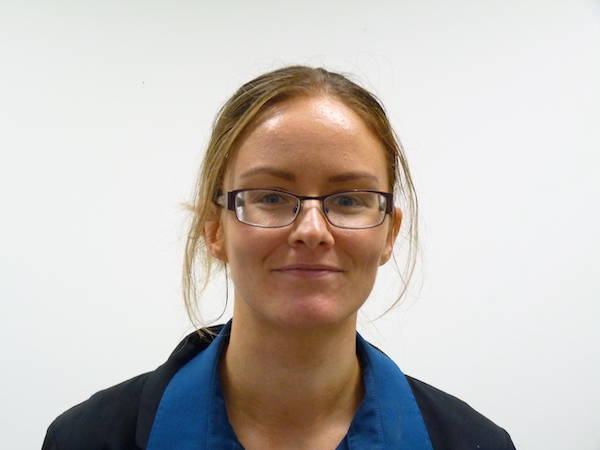
\includegraphics[width=\mugwidth]{img/laura.JPG}} & Member of Workgroup 4: Inclusion and Belonging\\

\addlinespace
\hdashline


Joanne Murphy (F) Administrative Officer &   
\adjustbox{valign=t}{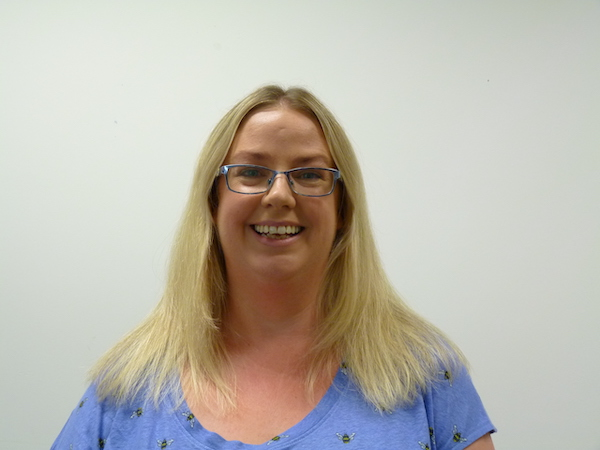
\includegraphics[width=\mugwidth]{img/joanne.JPG}} & Member of Workgroup 4: Inclusion and Belonging\\

\addlinespace
\hdashline

Sabin Tabirca (M) Senior Lecturer, Supervisor at ADVANCE-CRT, Coordinator of the Munster Programming Training (MPT) & 
\adjustbox{valign=t}{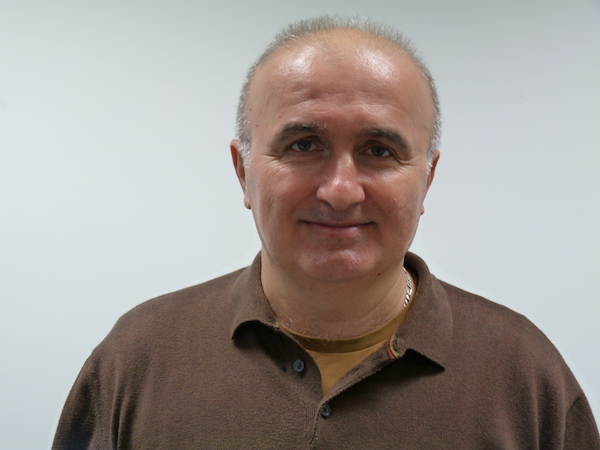
\includegraphics[width=\mugwidth]{img/sabin.JPG}} & Member of Workgroup 4: Inclusion and Belonging\\

\addlinespace
\hdashline
  
Ahmed Zahran (M) Lecturer, Course Director MSc Data Science and Analytics (MScDSA), Funded Investigator Connect Research Centre, Supervisor at ADVANCE-CRT &
\adjustbox{valign=t}{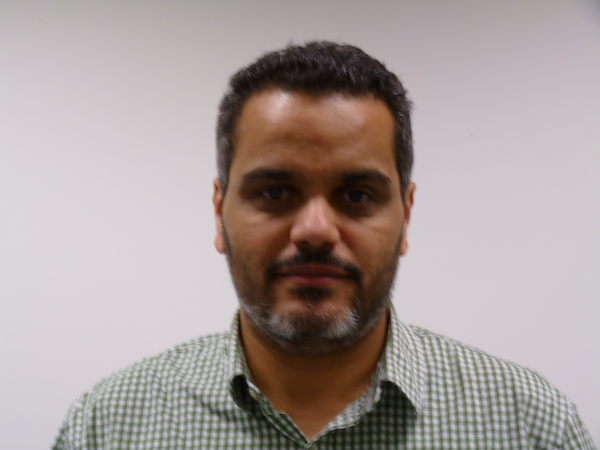
\includegraphics[width=\mugwidth]{img/ahmed.JPG}} & Member of Workgroup 4: Inclusion and Belonging\\

\bottomrule 


\end{longtable}
\end{mdframed}

%TC:endignore


\subsubsection{Information on how the chair was appointed and on what supports or resources the institution and/or department has given the chair to lead the self-assessment process}

Following an open invitation, in March 2021, 
the \ac{HOS} appointed Prof. Morrison to SAT Chair. Prof. Morrison has over 30 years experience of successfully leading large national and international research programmes and was recognised in 2017 by Enterprise Ireland as a Champion of EU Research. 
The Chair was supported by the School Manager and the Workgroup Liaison, who liaised with WG Chairs to analyse and visualise data, and compiled the application document.



\subsubsection{Comment on whether the self-assessment team is representative of the department, including if there is adequate representation of senior staff}

All of the female academic staff members and over 50\% of female PMS staff were members of the SAT. 
In total 41\% of the SAT were female.
Six members (21\%) of the SAT were senior staff, including 3 Professors, 1 Senior Lecturer, 1 Systems Administration Manager, and 1 School Manager. 


\subsection{Provide information on the preparation and delivery of this application by the department. This should include:}
\instr{
\begin{itemize}
\item an overview of the approach taken to evidence-gathering and analysis. Details of consultation response rates, disaggregated by gender, should be provided;
\item	information on plans for evaluating progress, including action plan implementation, over the coming four-year period. This should make reference to how often the SAT will meet, and how SAT succession and turnover will be planned and managed; 
\item	information on how the findings and activity of the self-assessment team are, and will continue to be, communicated to senior management and the wider department.
\end{itemize}
}


\subsubsection{An overview of the approach taken to evidence-gathering and analysis. Details of consultation response rates, disaggregated by gender, should be provided}

The SAT held several orientation meetings in April and May of 2021 to understand the scope of the AS process and to share ideas and experiences. Meetings were also held between UCC's EDI unit and the SAT Chair. 


At the time the SAT was formed, Covid-19 restrictions were in full force. A Microsoft Teams channel was created for the SAT, and all SAT meetings were conducted online.
All staff responded positively to the challenges of working remotely.


The SAT began working with the standard survey provided by the EDI unit; this was augmented to allow for more in-depth feedback.
Questions were added on parental leave, on experiences of new staff and on experiences of staff from under-represented groups. 




\begin{tabbox}{!t}

\caption{Survey response by gender, compared to total School staff count and gender distribution, and response rate by gender}
\label{tab:response:bygender}
\sisetup{
    group-digits=all,
    group-minimum-digits=4,
    group-separator = {,},
    table-format=4.1,
    mode=text,
    reset-text-series = false, 
    text-series-to-math = true,
    reset-text-family = false, 
    text-family-to-math = true
}
\footnotesize   
\begin{tabular}{p{4.5cm} 
                !{\qquad}
                S[table-format=2.0]
                !{\quad}
                S[table-format=2.1\%]
                p{0.5cm}
                S[table-format=2.0\%]                 
                !{\quad}
                S[table-format=2.1\%] 
                !{\qquad}
                S[table-format=2.1\%]                 
                } 

\toprule 
    & \multicolumn{2}{c}{\makecell{Gender representation\\of survey respondents}} 
    &
    & \multicolumn{2}{c}{\makecell{Gender representation\\of all staff School of CSIT}} 
    & {\multirow{2}{2cm}{\makecell{Overall\\Response\\rate}}}\\
    \cmidrule{2-3}\cmidrule{5-6}
Gender & {Count} & {\%} && {Count} & {\%} &  \\ 
\midrule 
Female & 16 & 28.6\% &&  19 & 23.5\% & 84.2\%\\
\hdashline
Male & 37 & 66.1\% && 62 &  76.5\% &59.7\%\\
\hdashline
Prefer not to say & 3 & 5.4\% && {n/a} & {n/a} & {n/a}\\
\midrule 
Total & 56 & 100.0\% && 81 & 100.0\% &69.1\%\\
\bottomrule 
\end{tabular}


\end{tabbox}


% \begin{SCfigure}[10][!ht]
% \hspace{-3pt}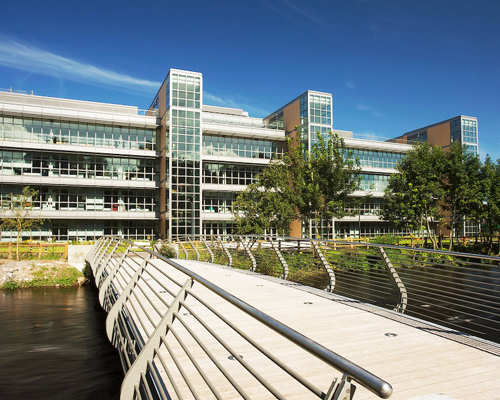
\includegraphics[width=3in]{img/WGB.jpg}
% \caption{Western Gateway Building: home to CSIT}
% \label{fig:wgb}
% \end{SCfigure}




\begin{tabbox}{!th}
\caption{Survey response by role}
\label{tab:response:byrole}
\sisetup{
    group-digits=all,
    group-minimum-digits=4,
    group-separator = {,},
    table-format=4.1,
    mode=text,
    reset-text-series = false, 
    text-series-to-math = true,
    reset-text-family = false, 
    text-family-to-math = true
}
\footnotesize   
\begin{tabular}{p{6.0cm} 
                !{\qquad}
                S[table-format=2.0]
                !{\quad}
                S[table-format=2.1\%]
                p{0.5cm}                
                S[table-format=2.0]
                !{\quad}
                S[table-format=3.2\%]
                p{0.5cm}                
                S[table-format=2.0]
                !{\quad}
                S[table-format=3.1\%]
                }

\toprule 
&\multicolumn{2}{c}{\makecell{Total survey\\ responses}}&&\multicolumn{2}{c}{\makecell{Female survey\\responses}}&&\multicolumn{2}{c}{\makecell{Male survey\\ responses}}\\
\cmidrule{2-3}\cmidrule{5-6}\cmidrule{8-9}
Category & {Count} & {\%} && {Count} & {\%} && {Count} & {\%}\\
\midrule 
Professional, Managerial and Support Staff & 14 & 25.0\% && 8 & 50.00\% && 6 & 16.2\%\\
\hdashline
Research Staff	& 16	 & 28.6\%	& & 7	& 43.75\%	&& 9	& 24.3\%\\
\hdashline
Academic Staff	& 21	& 41.1\%	&& 1 &	6.25\%	&& 20	&54.1\%\\
\hdashline
Teaching Staff	& 2	& 5.4\%	&& 0	& 0.00\%	&& 2	& 5.4\%\\
\midrule
Total & 53\textsuperscript{1} & 100.0\% && 16 & 100.00\% & & 37 & 100.0\%\\
\bottomrule 
\end{tabular}
{\\[.1in]
\sffamily
\textsuperscript{1} Three respondents preferred not to state their gender, which explains the discrepancy with Table~\ref{tab:response:bygender}.
}
\end{tabbox}

There were 56 responses, giving a participation rate of 69\%.  The response rates by gender for academic and \ac{PMS} staff reflect the gender balance in the school. Tables~\ref{tab:response:bygender} and \ref{tab:response:byrole} present the response rates by gender and by role. Those who did not disclose their gender (`prefer not to say') did not identify their role in the school. 

Responses to certain questions were low.
Following an invitation to all staff, 12 colleagues participated in 
three focus group sessions (for academic, PMS, and research staff) that were organised in May-June 2022, covering the following topics:

\begin{enumerate}[noitemsep]
\item Flexible working;
\item Support for colleagues with caring obligations; 
\item Support for career progression and development; 
\item School culture.
\end{enumerate}



Furthermore, four one-on-one interviews were undertaken with School Management.
Institutional data were provided by \ac{HR} and Central Academic Services. The university's EDI unit mediated all data, ensuring proper procedures and policies were applied.  



All WG activity and meeting minutes were stored and shared through the dedicated Microsoft Teams channel. This unrestricted access to data helped to support communications across the entire SAT. 


Each WG met weekly. The Chair's Workgroup met fortnightly, briefed each other on the activities of the previous period, coordinated cross-cutting WG activities, and planned actions for the coming period. 
The entire SAT met monthly and were briefed by the WG Chairs. Feedback from the entire SAT was invited, and was considered by each WG in subsequent meetings. Every effort was made to ensure that the SAT meetings were inclusive and open to diverse opinions.
The SAT meetings were timed to precede the monthly school meeting, where an update on SAT activities was a standing item on the agenda.
Figure~\ref{fig:timeline} shows the SAT activity timeline.

Members of the SAT took part in the online AdvanceHE training seminars and colleagues from schools and universities who were successful in achieving AS accreditation gave generously of their time to talk to the SAT and to share their experiences, including Professor Ita Richardson (University of Limerick), and Professor Lucy Hederman (Trinity College Dublin).







\subsubsection{Information on plans for evaluating progress, including action plan implementation, over the coming four-year period. This should make reference to how often the SAT will meet, and how SAT succession and turnover will be planned and managed}

In 2023,  the school structure will be augmented with the \ac{EDIIC}, thus replacing the AS SAT. It will be chaired by a senior member of staff and having male and female representation from academic, \ac{PMS}, and research staff (Action~\ref{action:intro:edi}). 



\begin{actionblock}{\ksspace{}Establish an EDI Implementation Committee}{intro:edi}
\actintroedi
\hfill{
    \hypersetup{hidelinks}
    \hyperlink{a2}{\gotoactionsymbol{}}
}
\end{actionblock}



Succession planning and turnover of the EDIIC membership will be managed by the \ac{HOS}, biennially using the same mechanisms for all other administrative appointments. Each member of the EDIIC will be also be a member of one of the School Standing  Committees: the \ac{APCD}; the Graduate Studies; Outreach; Research; Teaching and Learning; and the Student Experience. There they will act as an EDI champion, highlighting issues of concern.


\begin{landscape}

\begin{figbox}[20cm]{!ht}

    \caption{Timeline of events}
    \label{fig:timeline}
    % left low right up
    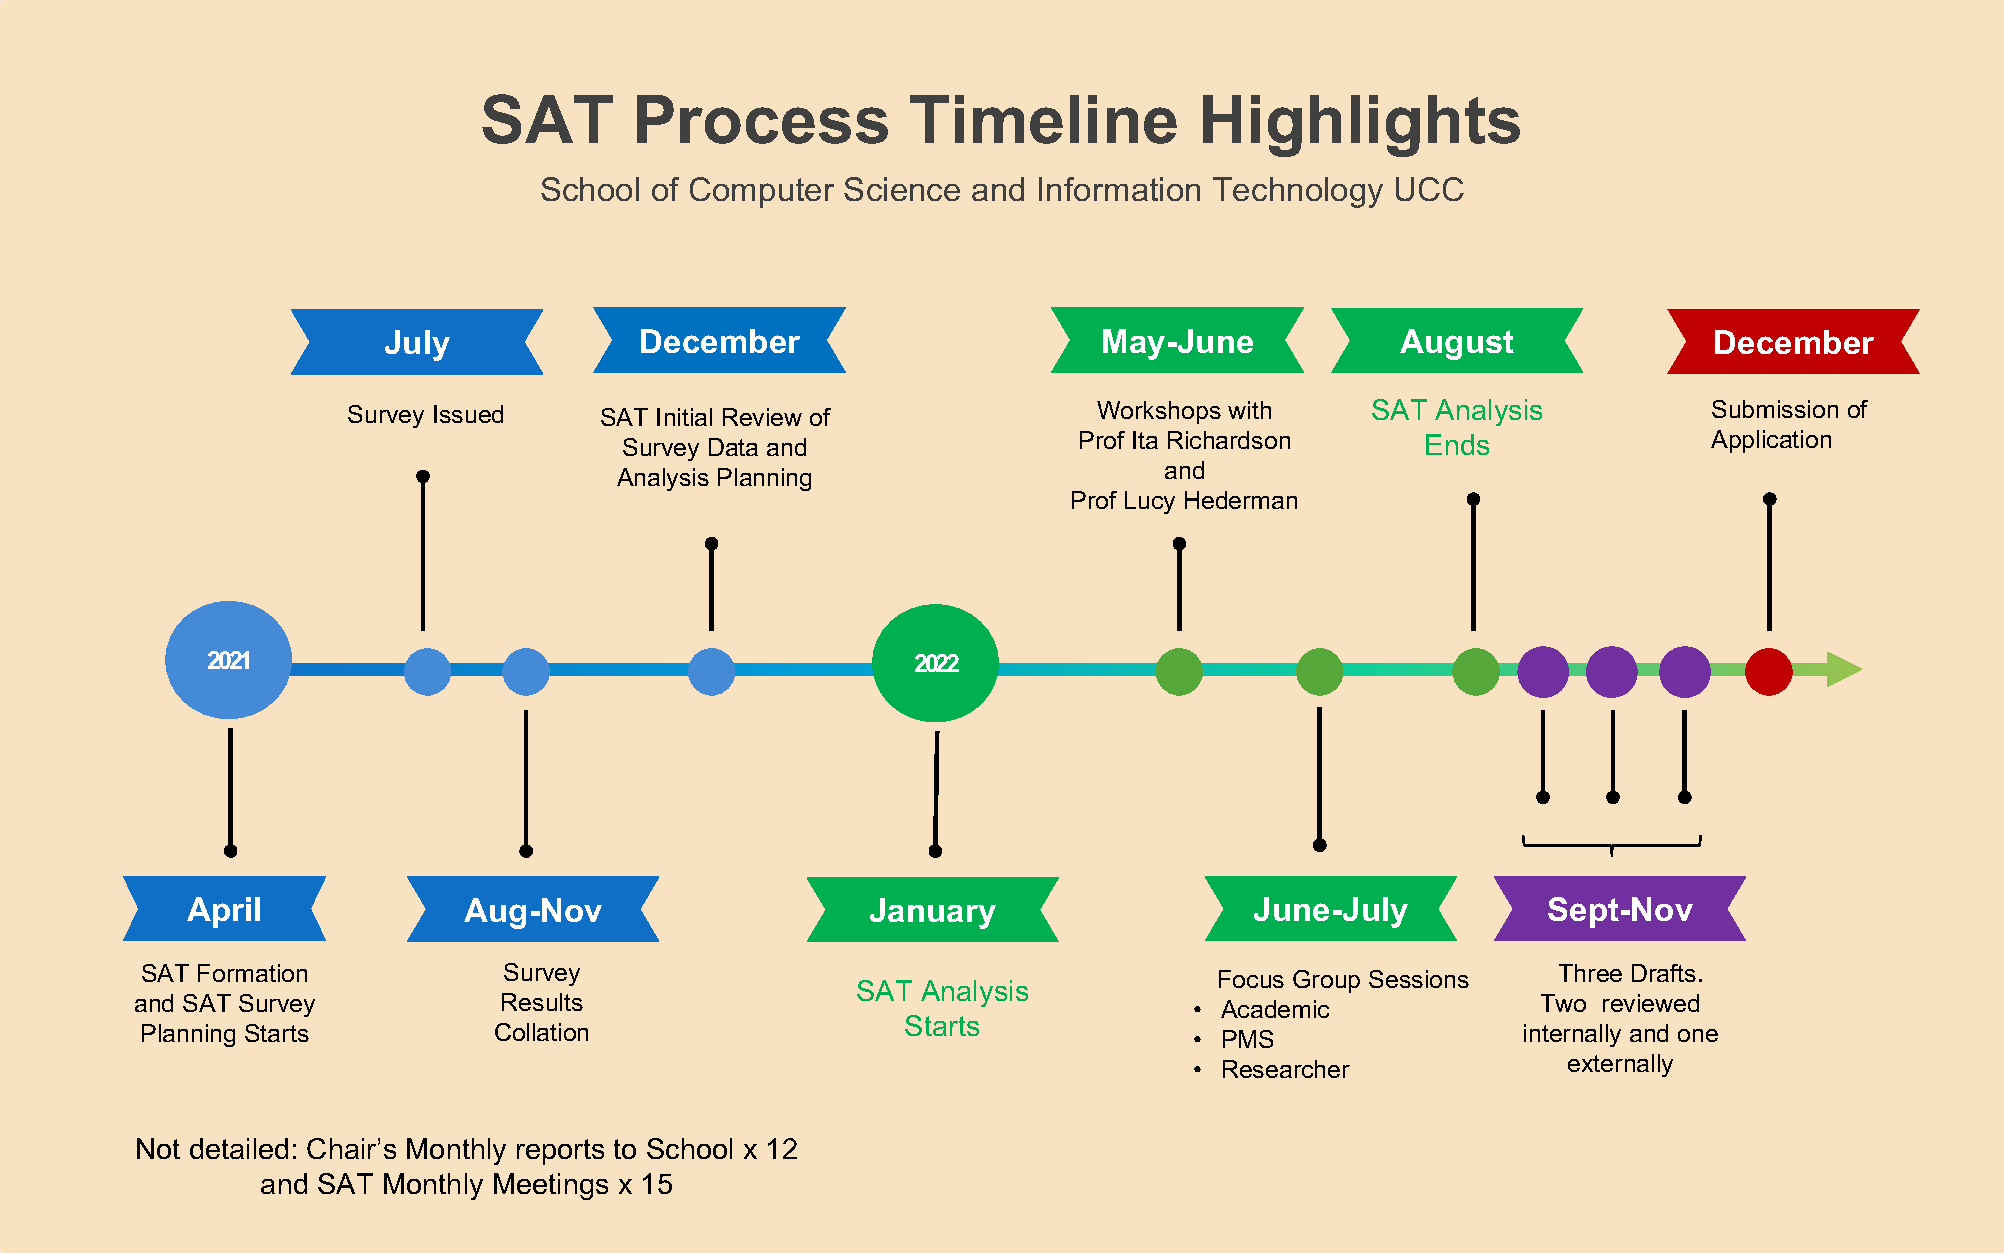
\includegraphics[trim={3mm 3mm 3mm 3mm},clip,width=20cm]{fig/timeline2.pdf}
    
\end{figbox}

\end{landscape}





\subsubsection{Information on how the findings and activity of the self-assessment team are, and will continue to be, communicated to senior management and the wider department}

The EDIIC will be responsible for evaluating progress and for overseeing the implementation of the action plan.
The EDIIC will meet monthly, to review progress, measure success and impact and take any actions necessary to progress the action agenda. The EDIIC Chair will report bi-annually to the school (Action~\ref{action:intro:agenda}).
The EDIIC will act as the main conduit between the school and  the College's EDI committee.



\begin{actionblock}{\ksspace{}Continuous updates to school}{intro:agenda}
\actintroagenda
\hfill{
    \hypersetup{hidelinks}
    \hyperlink{a5}{\gotoactionsymbol{}}
}
\end{actionblock}




In addition, to gauge the cultural impact of the AS implementation plan on staff and students, the EDIIC will conduct a review in 2026
(Action~\ref{action:intro:review:year3}).

\begin{actionblock}{\ksspace{}Review AS impact Year 3}{intro:review:year3}
\actreviewimpactyearthree
\hfill{
    \hypersetup{hidelinks}
    \hyperlink{a6}{\gotoactionsymbol{}}
}
\end{actionblock}











\chapter[An assessment of the department's gender equality context and wider equality context]{An assessment of the department's\\gender equality context and wider\\equality context}\label{chap:school}

\instr{In Section 2, applicants should evidence how they meet Criterion B:
\begin{itemize}
\item Evidence-based recognition of the issues and opportunities facing the applicant
\end{itemize}

Recommended word count: 8,000 words
}

%
% Modified Friday, 11 November (KH)
%



\section{Overview of the department and its context}
\label{sec:overview}


% The School comprises around 80 staff across all categories and grades
% as well as close to 700 students ranging from undergraduates to PhD 
% students These numbers include those belonging to a number of large 
% research groups/centres in the school.
% This includes Insight whose research focus is on constraints,
% AI and data analytics
% and also includes Connect devoted to research broadly
% on networks and communication technologies. 
% These two centres account for a significant 
% proportion of the school's research students and staff.


\subsection{Provide a description of the department's structures to advance equality. This should include:}  
\instr{
\begin{itemize}
\item teaching and research focus, including discipline coverage and any areas of specialism;
\item	the total number of staff by gender and category of post; 
\item	the total number of students by programme type and gender;
\item	information on location/s.
\end{itemize}
}

\subsubsection{Teaching and research focus, including discipline coverage and any areas of specialism}



Table~\ref{tab:teachingoverview} presents an overview of the school's
main teaching activities. 
The school has strategically diversified its portfolio in the
last decade by introducing a suite of interdisciplinary programmes
(denoted \interdis)
in Data Science (BScDSA and MScDSA), Digital Humanities (BADHIT) and Psychology and Computing (BAPC), designed to increase 
student  numbers overall and  particularly to improve gender balance. 


\input{tables2/tab_teaching_focus_25oct}

Research in the school falls into four thematic areas:
\begin{enumerate}[noitemsep]
    \item Artificial Intelligence, Data Analytics and Algorithmics
    \item Networks, Computer Architectures and Software Systems 
    \item Interactive Media and Human Computer Interaction
    \item Security, Privacy and Ethics
\end{enumerate}

The bulk of this activity is concentrated in  research groups 
and centres such as Insight 
and Connect 
(Table~\ref{tab:researchcentres}) 
and two centres for research 
training (CRTs, see  Table~\ref{tab:crts})
hosted within the school. 

\input{tables2/tab_research_centres_new}
\vspace{-4mm}
\input{tables2/tab_crts_new}


\subsubsection{The total number of staff by gender and category of post}

Table~\ref{tab:headcount} provides a snapshot of staff numbers 
in the school. Professional, Managerial, and Support Staff (PMS) 
includes those in administrative roles and in IT support roles.
Researchers includes only those who conduct research; those in
research support roles are classified as PMS, as their work and
concerns align more  closely with other PMS staff. Some
have permanent PMS posts in UCC, but are acting in more senior 
roles within research centres.



% KH note on data:
% Staff data are taken from Table A of EDI spreadsheet. When classifying
% staff I have adopted two conventions:
% 1) All core IT support staff (Dave's crew) are classified as "PMS"
% 2) "Research" staff (as listed in Table A) are split
%   [a] Those who conduct research directly as classified as "research"
%        (Research Assistant, Postdoc (incl MC), Senior Postdoc,
%         Research Fellow (incl MC) and Senior Research Fellow)
%   [b] Research support staff e.g. RSOs are classified as "PMS"
% 
\input{tables2/tab_headcount_29nov}

Females are under-represented in almost all categories, particularly 
in research and  academic roles. 
The school is acutely aware of this imbalance  and it is a strategic 
priority to address this over time.
This issue and some actions to address it  are explored in Section~\ref{sec:academic}.


\subsubsection{The total number of students by programme type and gender}


Table~\ref{tab:teachingportfolio} summarises student numbers by gender. 
\ac{CS} programmes internationally have  struggled with 
under-representation of females. Gender balance tends to
be better for interdisciplinary computing programmes. 



% \khcomment{Include to indicate trajectory is upwards.}
% 

\subsubsection{Information on location(s)}

Figure~\ref{fig:wgb} shows the Western Gateway Building (WGB) on campus,
the base for all CSIT staff and most activities. Before the school was relocated to the WGB in 2009, the school was dispersed across a number of locations. The single location provides far more opportunities for interaction.

\begin{figure}[!hb]
\caption[Western Gateway Building: home to CSIT]{Western Gateway Building: home to CSIT.}
\begin{tabular}{p{7cm}p{0.4cm}p{7cm}}
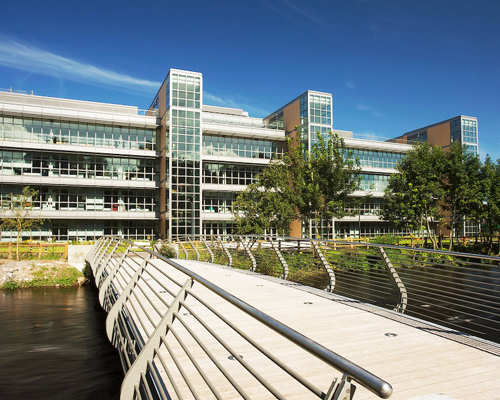
\includegraphics[align=t,height=2in]{img/WGB.jpg} 
&&
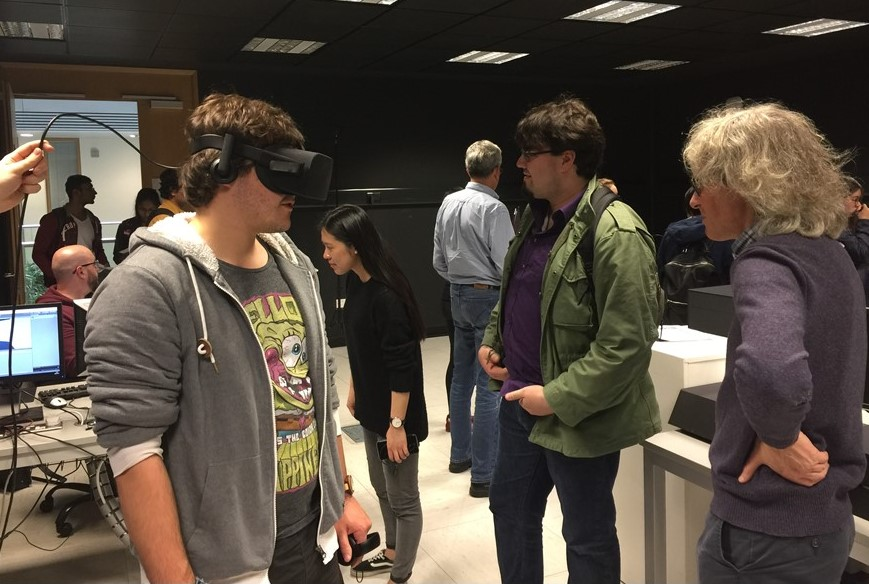
\includegraphics[align=t,height=2in]{img/vrlab.jpg}\\
\end{tabular}
\label{fig:wgb}
\end{figure}

\input{tables2/tab_taught_programmes_29nov}



\subsection{Analyse three years of data on undergraduate students by}
\label{sec:ug_data}
\instr{
\begin{itemize}
\item gender and degree programme, with reference to discipline-specific benchmark data; 
\item gender and degree attainment;
\item gender and foundation courses.  
\end{itemize}
}

\subsubsection{Gender and degree programme, with reference to discipline-specific benchmark data}

Figure~\ref{fig:ug:enrolment} summarises three years' enrolment statistics 
by gender for our undergraduate  programmes.\footnote{BScDSA and BAPC started  in 2018-19.} The figure shows a wide variation in
female enrolment rates from 14-16\% in the BScCS
to 44-50\% in BADHIT. The former aligns better
with the school's existing research strengths, so any increase 
in female undergraduate numbers there may provide a bigger 
pool of potential research postgraduates in time.

\begin{figbox}{!ht}
    \caption{Enrolment of undergraduate students 2017-2020}
    \label{fig:ug:enrolment}
    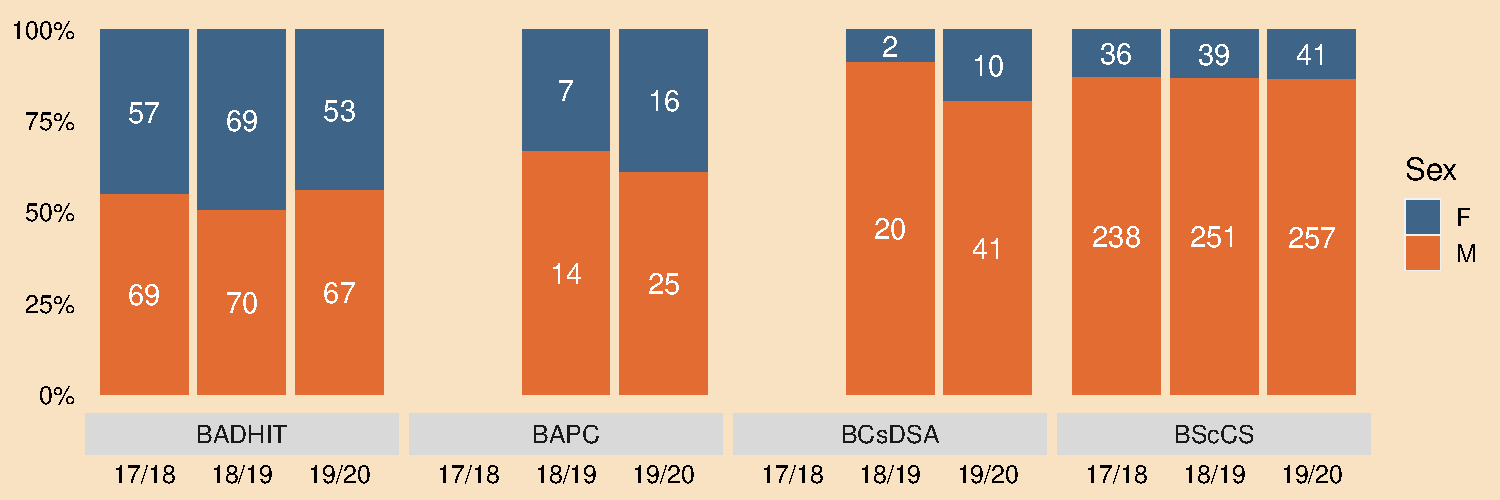
\includegraphics[width=\textwidth]{fig/ug_enrolment2.pdf}
\end{figbox}



Figure~\ref{fig:ug:mfintake} shows the evolution of the gender
breakdown linked to the introduction of new programmes
(BScDSA, BADHIT, BAPC). BADHIT and BAPC have improved 
the overall  gender balance.
In 2009-10, prior to the introduction of these newer 
programmes, the percentage of females was 14\%, compared 
with 24-25\% for the period shown.

\begin{figbox}{!t}
    \caption{Evolution of male/female intake for the BScCS programme vs. other undergraduate programmes within CSIT}
    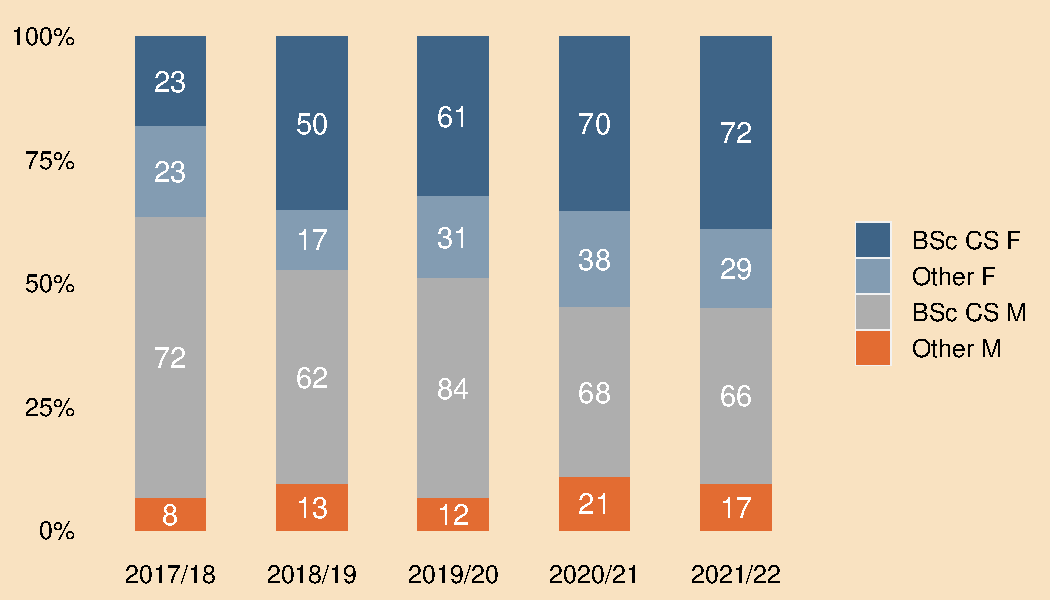
\includegraphics[width=5in]{fig/mfintake.pdf}
    \label{fig:ug:mfintake}
\end{figbox}

Table~\ref{tab:benchmarking:ug} compares CSIT's gender participation
rates for undergraduate  programmes with Irish (HEA) and UK (HESA)
benchmarks. CSIT's 22-24\% is somewhat better than the Irish (HEA) 
figure of 19-20\% and 15-16\% for the UK (HESA). 

\input{tables2/tab_benchmark_ug_25oct}

\subsubsection{Undergraduate gender and degree attainment}


Figure~\ref{fig:ug:attainment} summarises the degree classifications received  
by BScCS and BADHIT graduates for the years 2018-2020. (The first graduates for 
the other two undergraduate programmes emerged only in 2021-22.)


\begin{figbox}{!t}
    \caption{Degree attainment BScCS and BADHIT}
    \label{fig:ug:attainment}
    %\includegraphics[width=\textwidth]{fig/bsc_attainment2
    \begin{subfigure}[t]{2.9in}
    \caption{Degree attainment BScCS}
    \label{fig:bsc:attainment}
    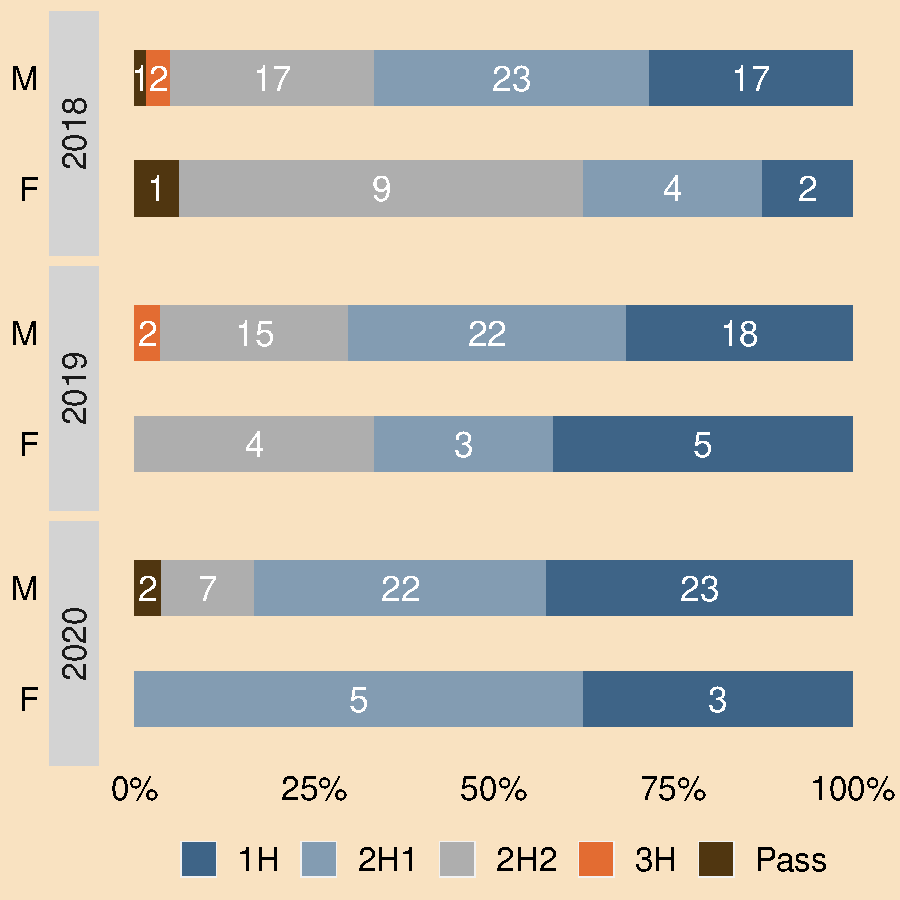
\includegraphics[width=2.8in]{fig/ug_attain2.pdf} % NEW
    \end{subfigure}
    %\includegraphics[width=4in]{fig/bsc_attainment2.pdf} %% OLD
    %
    \begin{subfigure}[t]{2.8in}
    \caption{Degree attainment BADHIT}
    \label{fig:badhit:attainment}
    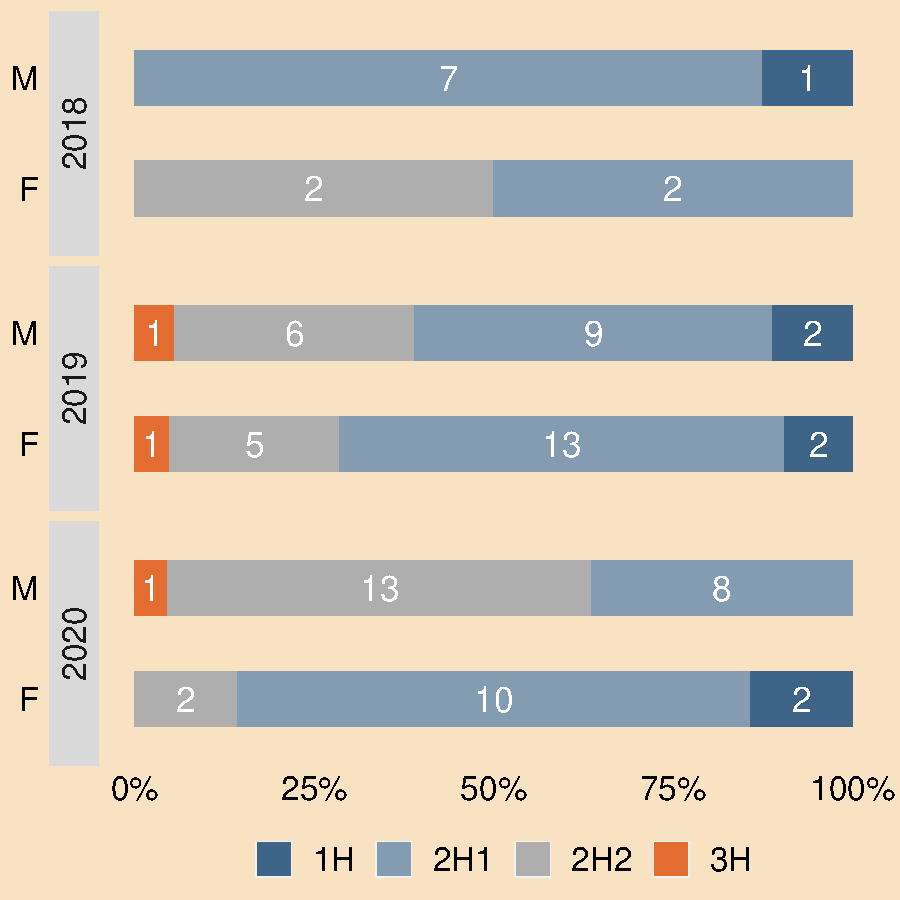
\includegraphics[width=2.8in]{fig/badhit_attainment.pdf}
    \end{subfigure}
    
\end{figbox}

Females are well represented among those  receiving higher degree classifications (Figure~\ref{fig:gradoftheyear}). The proportion of BADHIT female students receiving higher grades (2H1, 1H) was higher 
than their male classmates for two of the three years shown.
The Psychology \& Computing (BAPC) and Data Science \& Analytics (BScDSA) programmes only started in 2018; Figure~\ref{fig:ug:attainment:all} compares most recent degree attainment data across all four UG programmes.


\begin{figbox}{!t}

 \caption{Degree attainment undergraduate students across all 4 undergraduate programmes (2022)}
    %\centering
    \begin{subfigure}{2.8in}
    \caption{BScCS}
    \label{fig:attainment:bsccs}
    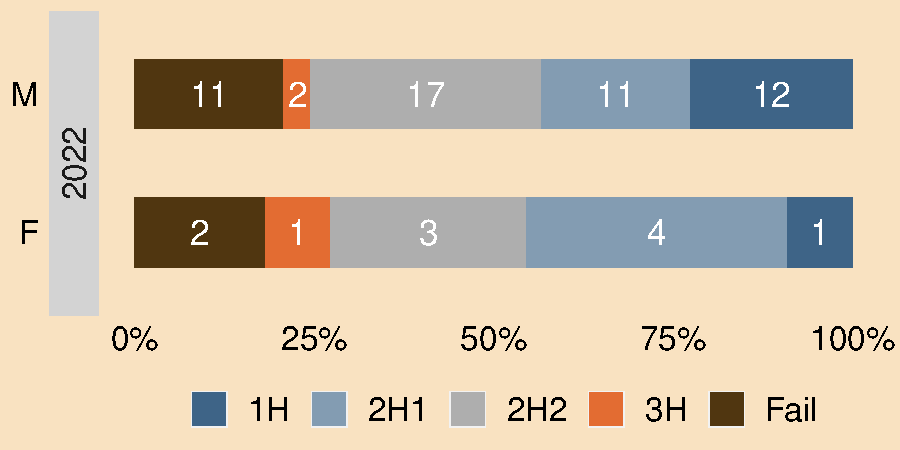
\includegraphics[width=2.8in]{fig/ug_attain_bsc22.pdf}
    \end{subfigure}
    %
    \begin{subfigure}{2.8in}
    \caption{BADHIT}
    \label{fig:attainment:badhit}
    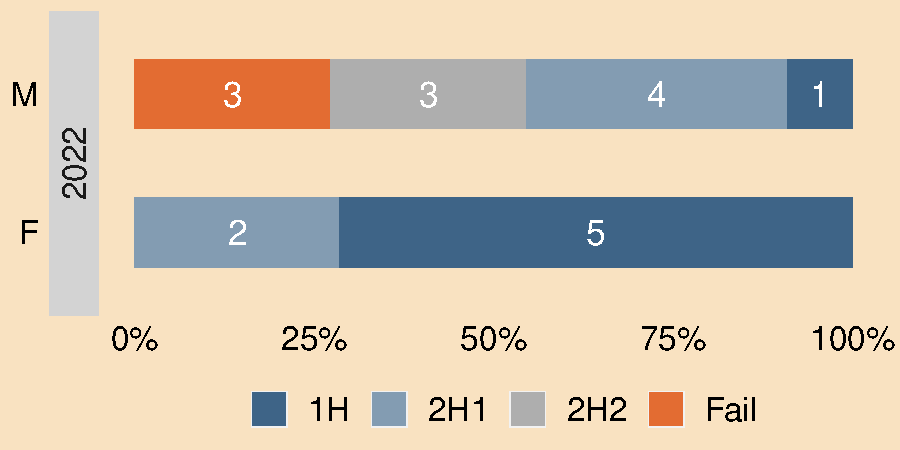
\includegraphics[width=2.8in]{fig/ug_attain_badhit22.pdf} 
    \end{subfigure}
    %
    \par\bigskip
    %
    \begin{subfigure}{2.8in}
    \caption{BAPC}
    \label{fig:attainment:bapc}
    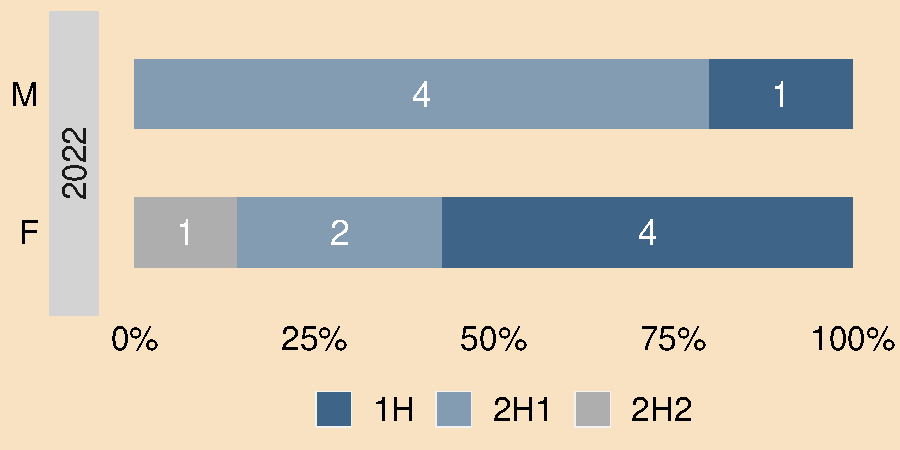
\includegraphics[width=2.7in]{fig/ug_attain_bapc22.pdf} 
    \end{subfigure}
    %
    \begin{subfigure}{2.8in}
    \caption{BScDSA}
    \label{fig:attainment:bscdsa}
    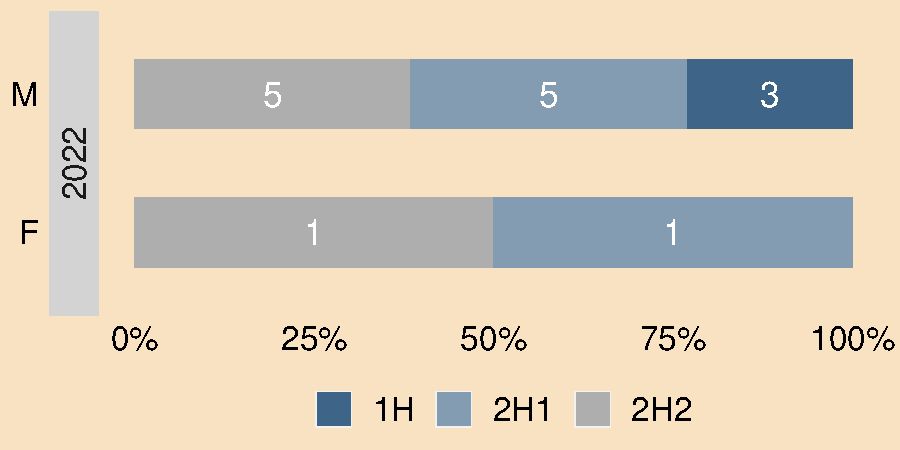
\includegraphics[width=2.7in]{fig/ug_attain_bscdsa22.pdf} 
    \end{subfigure}
    %
    \par 
    %% Add the legend
   

    
    \label{fig:ug:attainment:all}

\end{figbox}


\begin{figure}[!h]
\caption{Two CSIT undergraduate students receiving SEFS College Graduate of the Year (and runner-up) Awards.}
\label{fig:gradoftheyear}
\begin{tabular}{l !{\quad} r}

\includegraphics[height=2.15in]{img/eimearcrotty.jpg} &
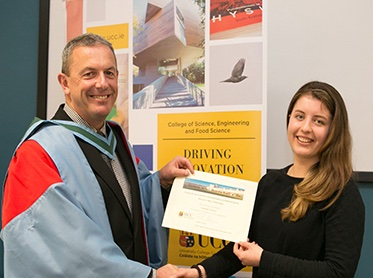
\includegraphics[height=2.15in]{img/cathbowen.jpg} \\

\end{tabular}
\end{figure}

\subsubsection{Undergraduate gender and foundation courses}

CSIT does not offer foundation courses.

\pagebreak 
\subsection{Analyse three years of data on postgraduate taught students by:} 
\instr{
\begin{itemize}
    \item gender and degree programme, with reference to discipline-specific benchmark data;  
    \item gender and degree attainment.  
\end{itemize}
}
\label{pg_data}


\subsubsection{Postgraduate taught student gender and degree programme, with reference to discipline-specific benchmark data}


Figure~\ref{fig:pg:enrolment} shows three years' enrolment data for our taught
postgraduate programmes. Female participation rates are generally better 
for postgraduate programmes than for undergraduate. The MScIM, which also attracts 
students with non-computing backgrounds, is the only programme
where females (56-68\%)  outnumber males. Both MScCS and MScDSA 
have a high proportion of non-EU students and a significantly 
better gender balance, possibly due to higher participation 
among females in STEM subjects in some non-EU countries.


\begin{figbox}{!ht}
    \caption{Enrolment postgraduate students 2017-2020}
    \label{fig:pg:enrolment}
    %\centering
    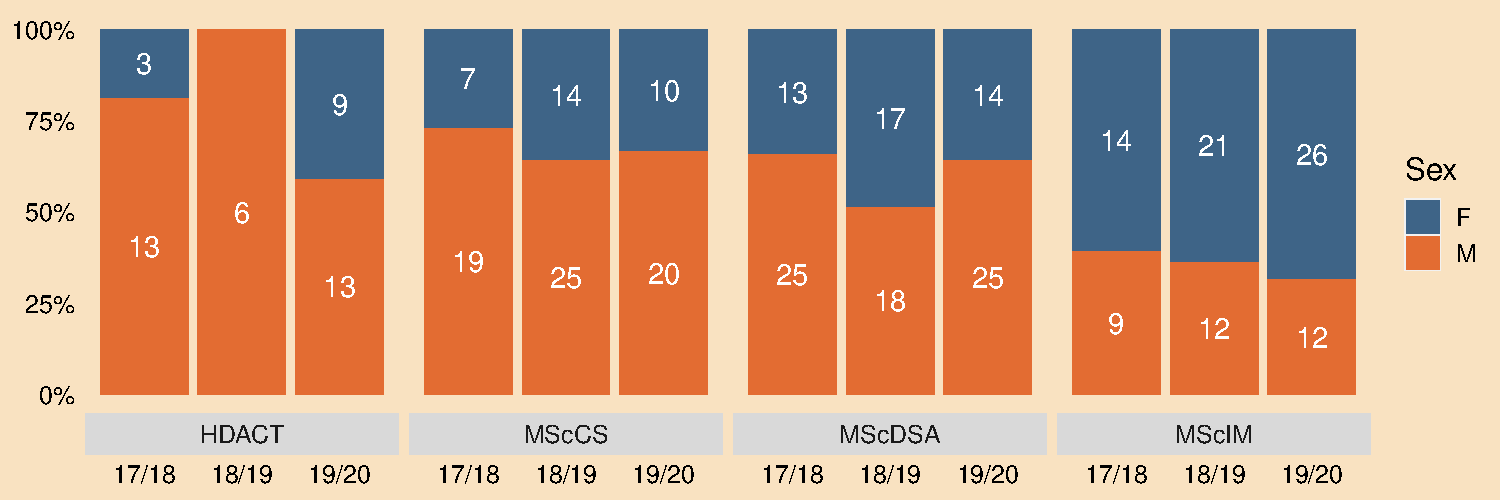
\includegraphics[width=\textwidth]{fig/pg_enrolment.pdf}
\end{figbox}


\input{tables2/tab_benchmark_pg_25oct}


Figure~\ref{fig:pg:enrolment} shows increased female enrolments in our postgraduate taught programme from  
37\% to 43\%. Table~\ref{tab:benchmarking:pg} shows  
CSIT to be higher (37-45\%) compared with national (HEA) figures and UK (HESA) 
figures of 29-32\% and 30-31\%, respectively.

\subsubsection{Postgraduate taught student gender and degree attainment}

Figure~\ref{fig:pg:attainment} plots three year's data on 
the degree classifications achieved for Postgraduate Taught (PGT) programmes; females feature prominently among those achieving
higher grades.

\begin{figbox}{!ht}

 \caption{Degree attainment postgraduate students}
    %\centering
    \begin{subfigure}{2.8in}
    \caption{Postgraduate attainment HDip ACT}
    \label{fig:hdip}
    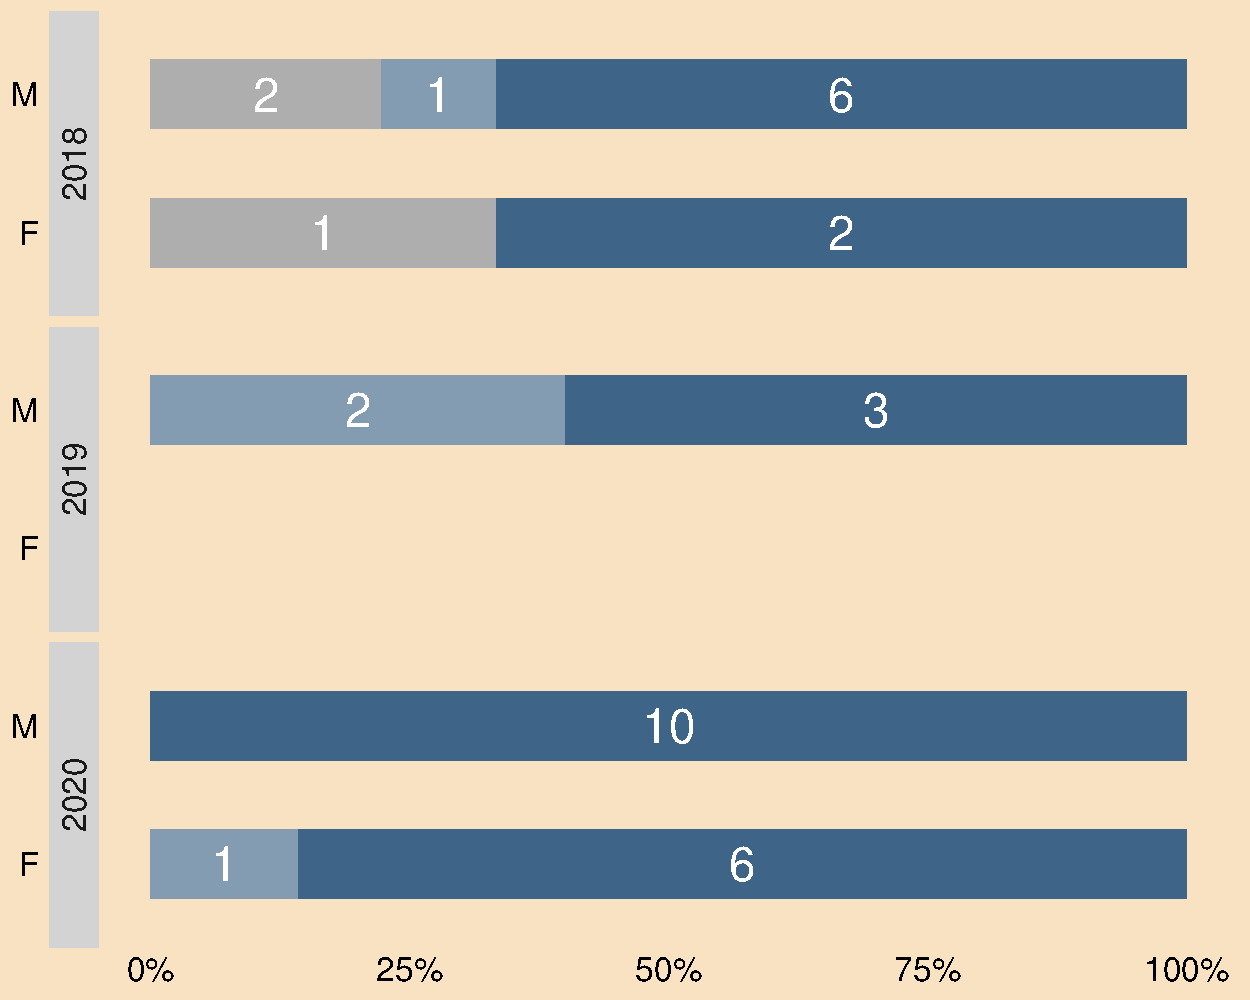
\includegraphics[width=2.8in]{fig/pg_hdact_attainment.pdf}
    \end{subfigure}
    %
    \begin{subfigure}{2.8in}
    \caption{Postgraduate attainment MSc CS}
    \label{fig:msccs}
    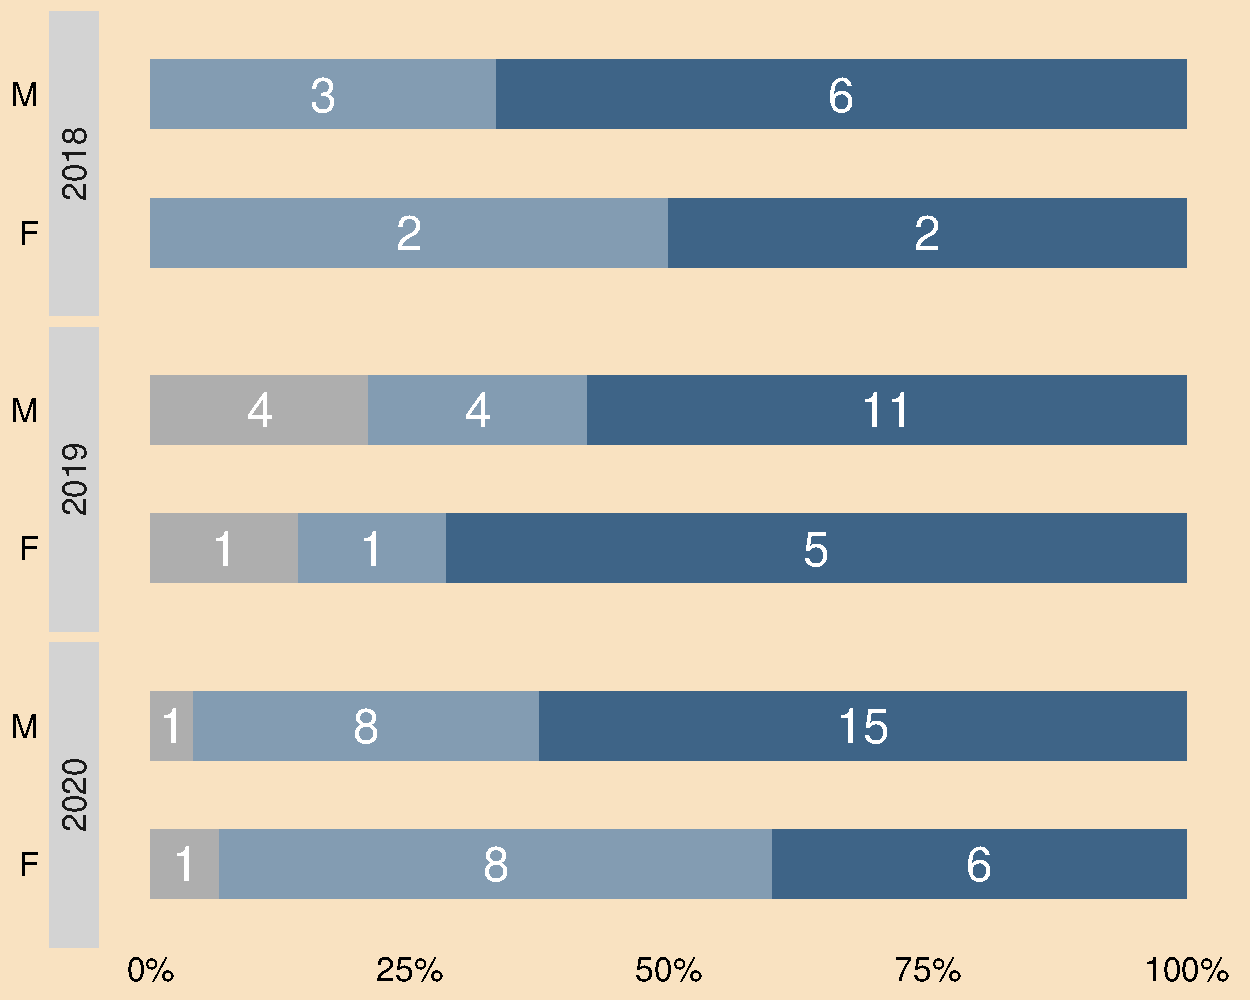
\includegraphics[width=2.8in]{fig/pg_msccs_attainment.pdf} 
    \end{subfigure}
    %
    \par\bigskip
    %
    \begin{subfigure}{2.8in}
    \caption{Postgraduate attainment MSc DSA}
    \label{fig:mscdsa}
    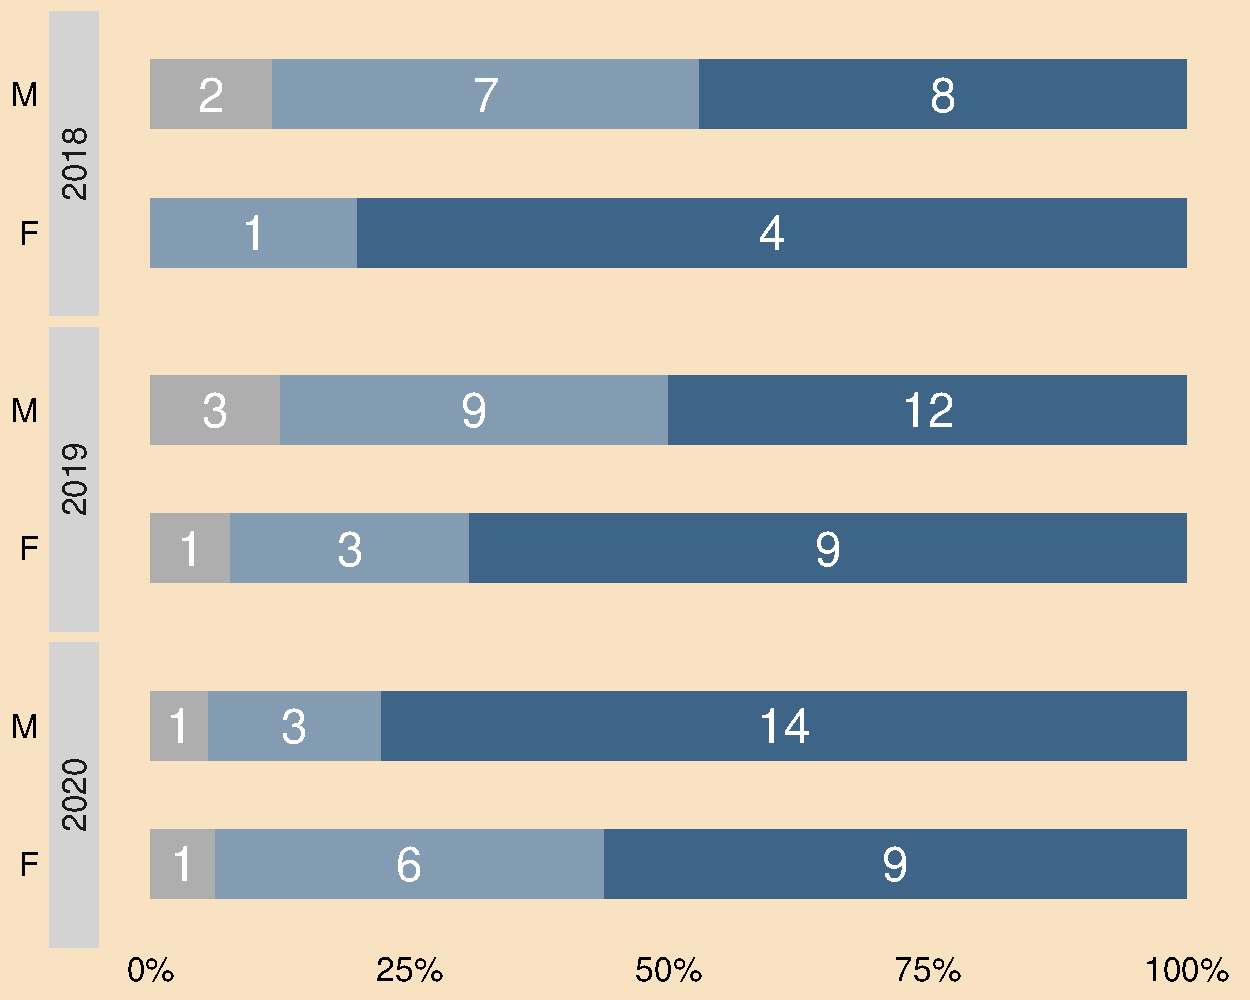
\includegraphics[width=2.7in]{fig/pg_mscdsa_attainment.pdf} 
    \end{subfigure}
    %
    \begin{subfigure}{2.8in}
    \caption{Postgraduate attainment MSc IM}
    \label{fig:mscim}
    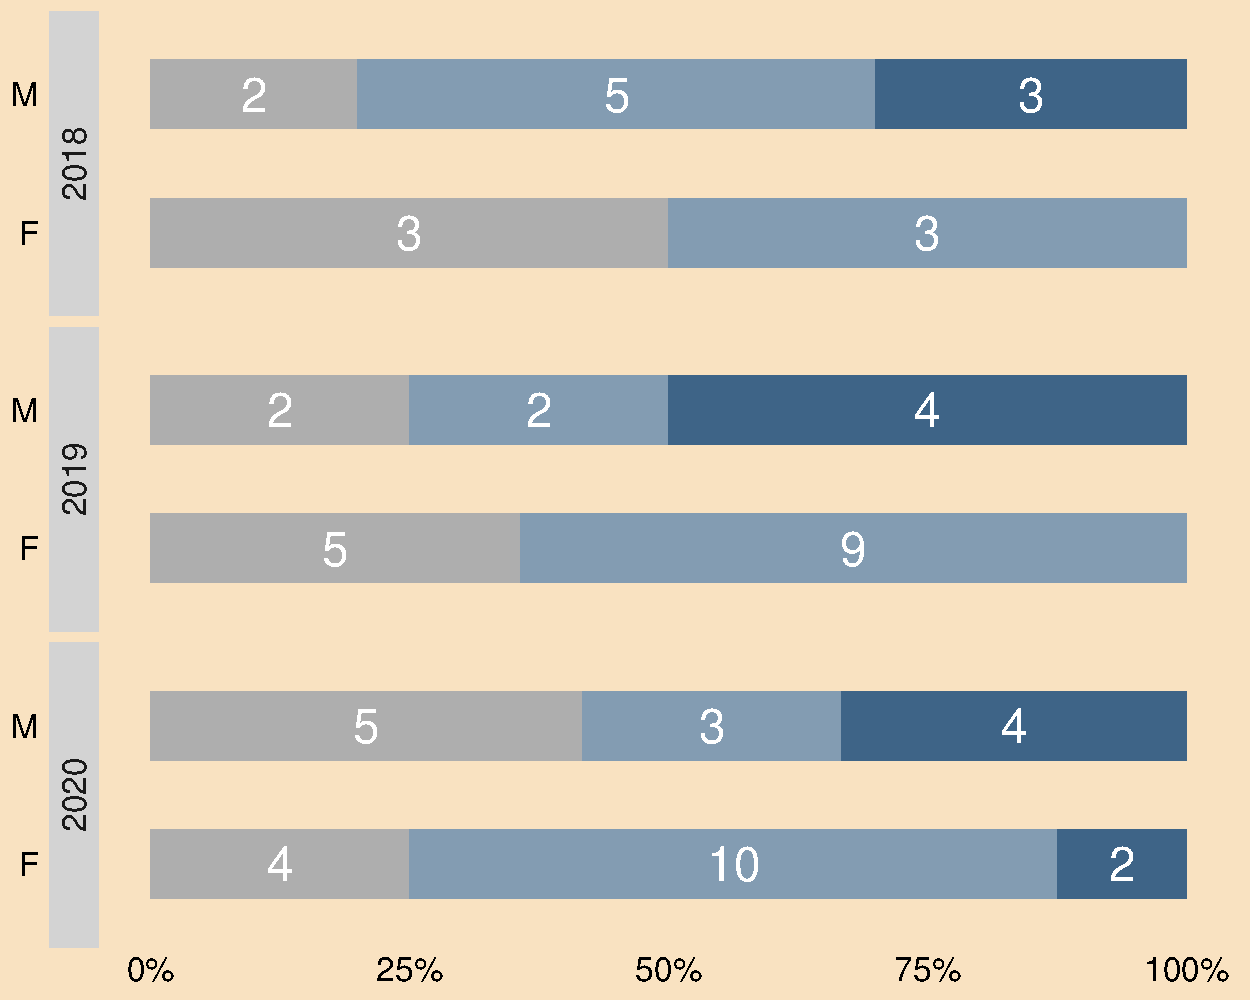
\includegraphics[width=2.7in]{fig/pg_mscim_attainment.pdf} 
    \end{subfigure}
    %
    \par 
    %% Add the legend
   
    \begin{subfigure}{14cm}
    \centering 
    % left bottom right top
    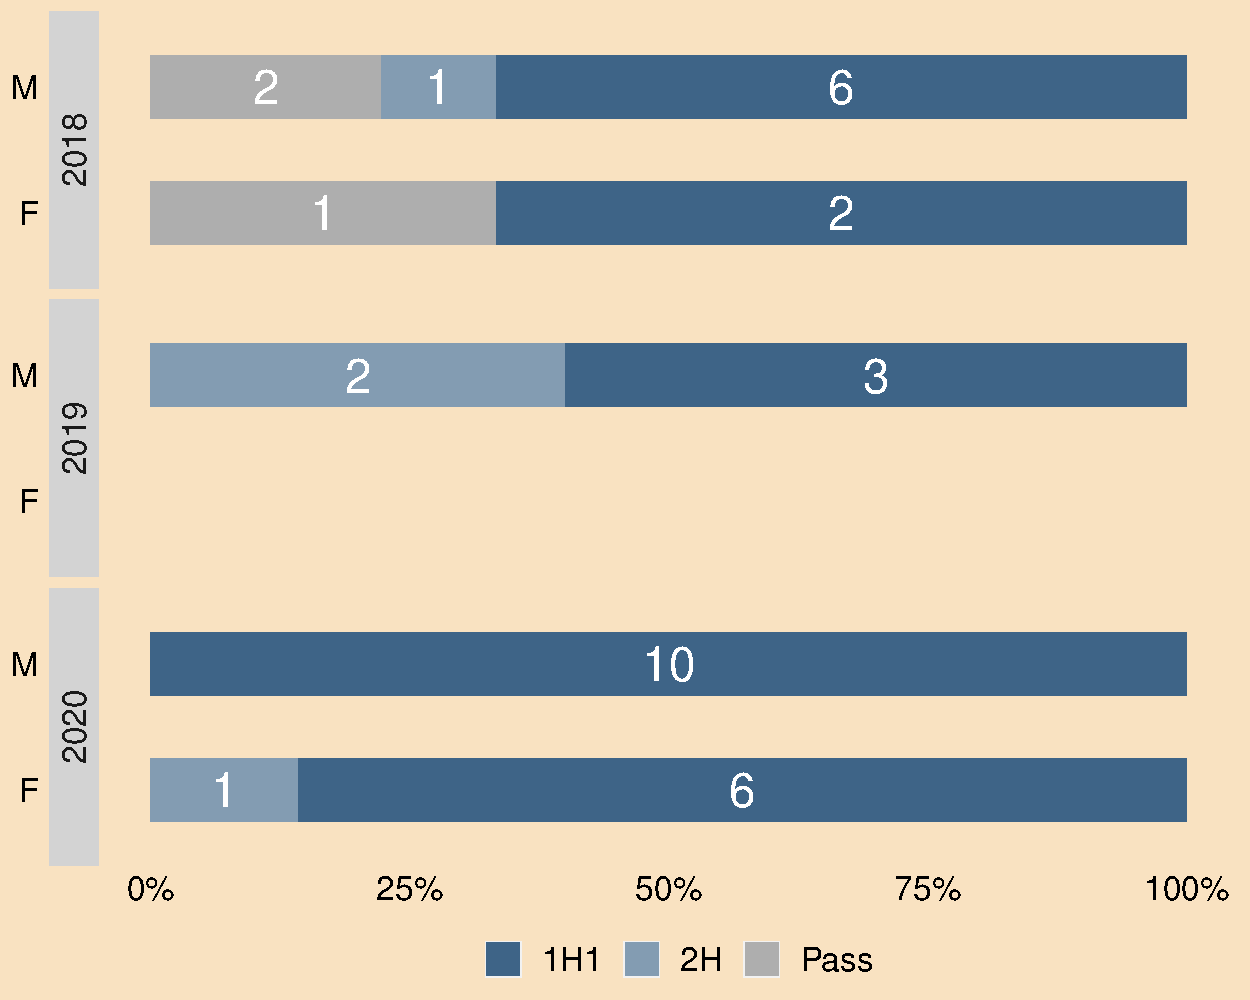
\includegraphics[trim={0 0 0 15.5cm},clip,scale=0.6]{fig/pg_legend.pdf} 
    \end{subfigure}
    
    \label{fig:pg:attainment}

\end{figbox}


\subsection{Analyse three years of data on postgraduate research 
students by:}  
\instr{
\begin{itemize}
    \item gender and enrolment; 
    \item gender and application, offer, and enrolment, with comment on how this data is collected and evaluated by the department, and on any gender disparities in student funding;  
    \item gender and completion rates.  
\end{itemize}
}
\label{sec:phdstudents}


\subsubsection{Postgraduate research student gender and enrolment}
\label{sub:phdnumbers}


Table~\ref{tab:phdregistrations} shows three years' data 
on postgraduate research students (virtually all PhDs). 
The dip in 2019-20 reflects the absence of funding before
the start of the CRTs.
%the ending of one funding source,
%before the start of the two Centres for Research Training (CRT). 
CRTs have explicit targets to 
increase female students (40\%) (Table~\ref{tab:phdintakerecent}). The percentage of females
among Postgraduate Research (PGR) students is significantly above that of the 
undergraduate population.
As SFI has gender targets attached to other funding, a similar 
pattern is expected among the non-CRT PGR intake in future years.



\input{tables2/tab_pgr_registrations_30nov}

\input{tables2/tab_pgr_intake_recent_30nov}

A snapshot of PhD intake  by research centre or 
CRT for 2022-23 is 
shown in Table~\ref{tab:phdregistrations2223}, indicating that gender balance is improving. Figure~\ref{fig:advance:cohort} shows the 2019 cohort of ADVANCE-CRT.

\input{tables2/tab_pgr_registrations_22_23_30nov}

\begin{figure}[!t]
\caption{ADVANCE-CRT cohort 2019}
\label{fig:advance:cohort}
\begin{tabular}{c !{\quad} c}

\includegraphics[width=3.6in]{img/Advance.JPG} &
\end{tabular}
\end{figure}

\subsubsection{Postgraduate research student gender and application, offer, and enrolment, with comment on how this data is collected and evaluated by the department, and on any gender disparities in student funding}
\label{sec:phdnumbers}


Historically, the PGR application process was handled by individual 
centres or PIs who maintain local 
records (see below). There has been no school-level  monitoring of number of applicants, offers 
and acceptances by gender. PGR application data will be collated under
Action~\ref{action:record:hiring:phd}.

\begin{actionblock}{\ksspace{}Collate postgraduate research application aata}{record:hiring:phd}
\acttrackgenderinfophd
\hfill{
\hypersetup{hidelinks}
\hyperlink{aa0}{\gotoactionsymbol{}
}}
\end{actionblock}

Table~\ref{tab:crtapplications} summarises the
number of applications and enrolments by gender for the two CRTs
since their introduction in 2019. 
The strategy of a quota of 40\% female enrolments has by and large been achieved in the CRTs.


\input{tables2/tab_crt_applications_25oct}






\subsubsection{Postgraduate research student gender and completion rates}

Table~\ref{tab:phdcompletionstats} shows data on
PhD completions (30\% female);
%and Table~\ref{tab:phdcompletionrates} shows 
%the completion rates (27\% female) for those expected to finish during 
%the three-years 2017-18 to 2019-20, assuming fours years to complete.
%Table~\ref{tab:phdcompletionstats} 
data were derived from
registration and graduation data.  
These figures may overstate completion 
times due to the
lag between ``finishing up'' (\emph{viva voce}, submission) 
and graduation.

\input{tables2/tab_phd_completion_stats_5dec}

Table~\ref{tab:phdcompletionrates} shows the completion rates (27\% female) 
for those expected to finish during the three-year reference 
period 2017-18 to 2019-20, assuming fours years to complete.

\input{tables2/tab_phd_completion_rates_28oct}


The average completion time was similar for both
genders (60\nicefrac{1}{4} (M), 63\nicefrac{1}{4} (F) months) and significantly 
above the 48 month target.
UCC's recently introduced policy on annual 
progress reviews for research students provides a 
framework for managing these issues.


\begin{figure}[!h]
\caption{Left: graduation day. Right: PhD Review Day}
\label{fig:postgrads}
\begin{tabular}{l !{\quad} r}

\includegraphics[height=1.88in]{img/graduation.jpg} &
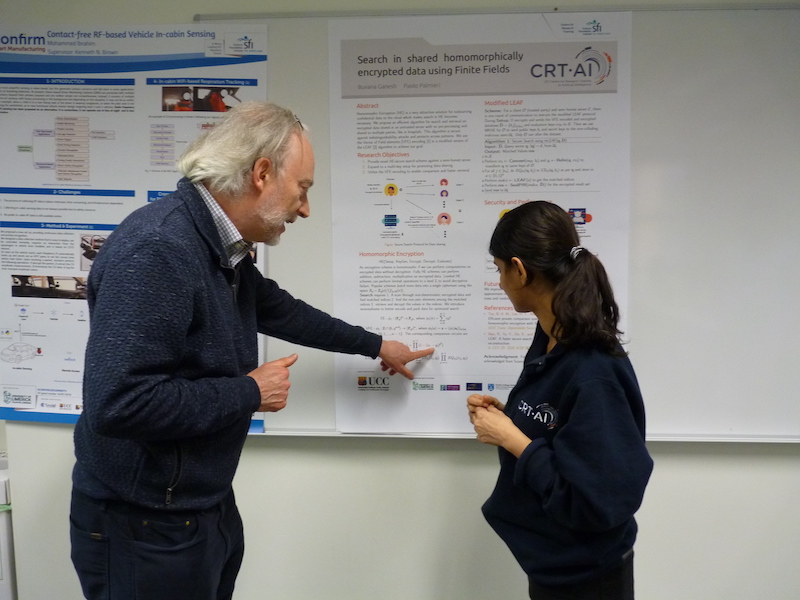
\includegraphics[height=1.88in]{img/phdreview1.JPG} \\

\end{tabular}
\end{figure}

\subsection{Comment and reflect on the relationship (if any) between the department's outreach, engagement, and support activities and issues or opportunities in the student pipeline. This should include comment on how the department recognises staff and student contributions to these activities and monitors the gender balance of those involved.}

The school participates in all
university outreach activities including Open Days 
and careers guidance briefings (Figure~\ref{fig:utzwithkids}). It also hosts
its own initiatives, including  annual information 
evenings, a very popular programme of weekend programming 
classes\footnote{Munster Programming Training (MPT)
\url{https://www.ucc.ie/en/csschools/mpt/}}
and summer camps,\footnote{\url{https://www.ucc.ie/en/csschools/ictsummercamp/}}
 aimed at second-level students, 
in addition to regular school visits 
(Table~\ref{tab:schoolvisits}). All activities are 
tailored to support diversity of undergraduate intake.

\input{tables2/tab_school_visits_18nov}


\begin{figure}[!t]
\caption[Outreach activities at CSIT]{From left to right: Outreach activities at CSIT. Head of School Prof Utz Roedig with potential future students. Visit from transition year students. Munster Programming Training. UCC Open Day.}
\label{fig:utzwithkids}
\begin{tabular}{c !{\quad} c}
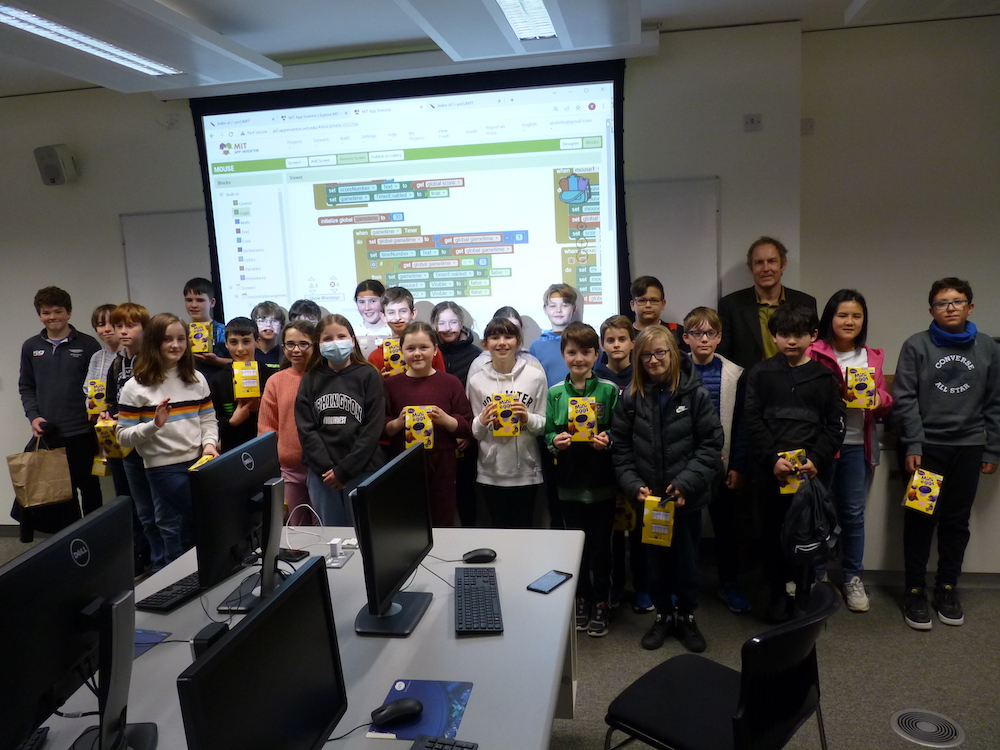
\includegraphics[width=2.85in]{img/utzwithkids.JPG} &
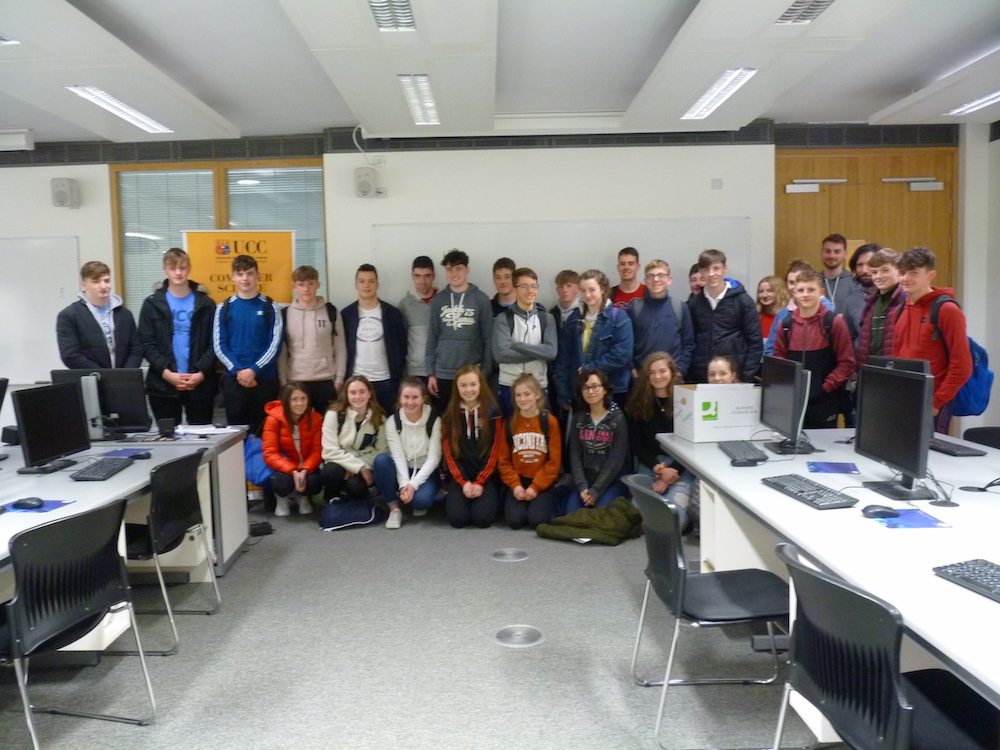
\includegraphics[width=2.85in]{img/futurestudents.JPG} \\
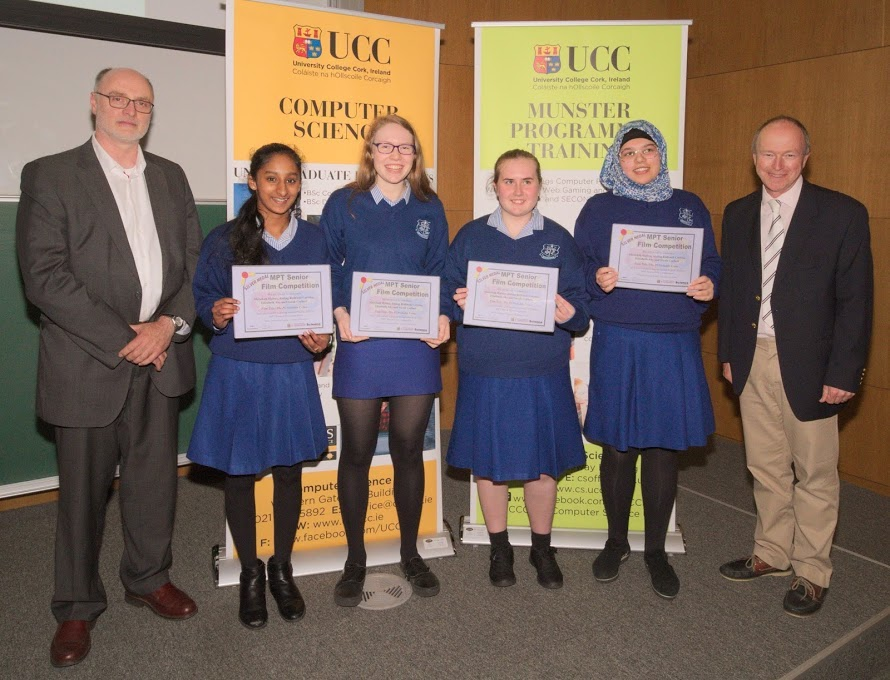
\includegraphics[trim={0 3mm 0 0},clip,width=2.85in]{img/winner_14 mount mercy_1.jpg} &
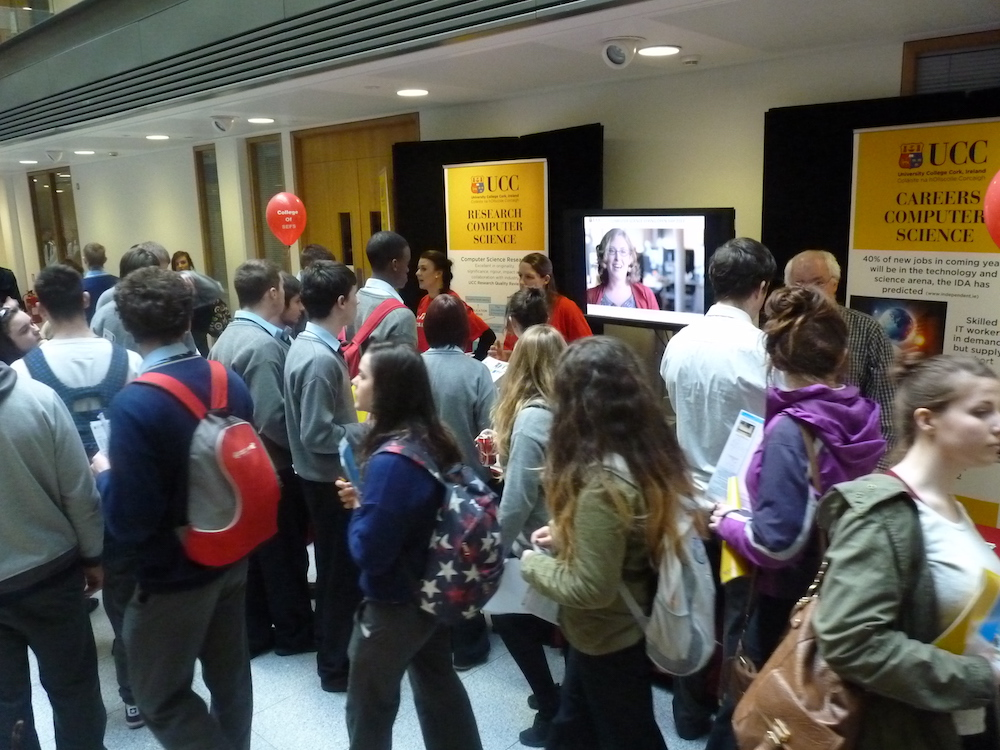
\includegraphics[width=2.85in]{img/openday.JPG} \\

\end{tabular}
\end{figure}

Our existing outreach, marketing and support measures
have evolved in an ad-hoc manner over the years; the 
current AS exercise has highlighted the need for
a comprehensive audit of these activities 
to assess their effectiveness and reflect on how they might 
be reconfigured to address the two key challenges in the 
student pipeline:
\begin{enumerate}[noitemsep]
\item  the under-representation of females in the BScCS and BScDSA 
(Table~\ref{tab:teachingportfolio}); 
\item the lack of female undergraduates who opt to 
progress to graduate research studies.
\end{enumerate}

A survey of current female undergraduates 
(Action~\ref{action:survey:females}) will help inform a 
review of existing marketing and outreach
activities and reconfigure these activities to improve
recruitment of females and to enhance diversity of intake
more generally (Actions~\ref{action:cult:diverseoutreach}
and \ref{action:review:outreach}).
Action~\ref{action:survey:females} will also  diagnose issues
with how the school projects itself to prospective undergraduates.


\begin{actionblock}{\ksspace{}Investigate female perceptions towards
Computer Science and careers}{survey:females}
\actsurveyugfemales
\hfill{
    \hypersetup{hidelinks}
    \hyperlink{b0}{\gotoactionsymbol{}}
}
\end{actionblock}



\begin{actionblock}{\ksspace{}Improve focus on diversity in outreach activities}{cult:diverseoutreach}
\actreviseoutreachpractice
\hfill{
    \hypersetup{hidelinks}
    \hyperlink{b6}{\gotoactionsymbol{}}
}
\end{actionblock}

\begin{actionblock}{\ksspace{}Re-assess and re-configure
existing outreach and support measures}{review:outreach}
\actreviewactivities
\hfill{
    \hypersetup{hidelinks}
    \hyperlink{b2}{\gotoactionsymbol{}}
}
\end{actionblock}



Linking with Action~\hyperlink{act511}{5.1.1}
of UCC's AS Action Plan 2019-2023,\footnote{\url{https://www.ucc.ie/en/media/support/edi/athenaswan/AthenaSWANUCCActionPlan2019-2023.pdf}}
Actions~\ref{action:genderproof:guidelines} 
and \ref{action:boost:visibility} 
will underpin  an overhaul of materials to help reshape recruitment 
materials for future academic, research and PMS vacancies 
(e.g. Action~\ref{action:acad:marketing} and 
Action~\ref{action:pms:matchdescription}).

\begin{UCCaction}{5.1.1}{}\hypertarget{act511}
Revise equality of opportunity statement in recruitment material to reflect a more inclusive, positive and specific commitment to equality principles Develop guidance for writing equality-focused post advertisements, including statements encouraging applications from the underrepresented groups.
\end{UCCaction}


\begin{actionblock}{\ksspace{}Develop gender proofing guidelines
for materials}{genderproof:guidelines}
\actgenderproof
\hfill{
    \hypersetup{hidelinks}
    \hyperlink{b1}{\gotoactionsymbol{}}
}
\end{actionblock}

\begin{actionblock}{\ksspace{}Boost visibility of females}{boost:visibility}
\actboostvisibility
\hfill{
    \hypersetup{hidelinks}
    \hyperlink{b3}{\gotoactionsymbol{}}
}
\end{actionblock}

The recent appointment of a dedicated mentor
has proved effective in improving student experience
for international students. A mentor for female undergraduate students 
will be appointed to offer 
guidance and support (Action~\ref{action:edi:coach}), help coordinate various female-focused 
initiatives,
and encourage female undergraduates to pursue career-enhancing
opportunities e.g., IGNITE entrepreneur incubation 
initiative,\footnote{\url{https://www.ucc.ie/en/ignite/}}
scholarships and internships aimed at  female 
undergraduates (e.g. Huawei, Google), 
participation in events, such as the Irish Programming Olympiad and 
the International Olympiad for Informatics and engagement
with organisations devoted to supporting young women in STEM
such as 
iWish,\footnote{\url{https://www.iwish.ie}}
WiSTEM\footnote{\url{https://www.facebook.com/UCCWiSTEM/}}
and IEEE Women in Engineering (Figure~\ref{fig:olympiad}).


\begin{figure}[!t]
\caption{From top left to bottom right: Irish Programming Olympiad; Huawei Scholarships; Google sponsorship of Irish Collegiate Programming Competition; UCC Quercus Talented Students Programme}
\label{fig:olympiad}
\begin{tabular}{c !{\quad} c}
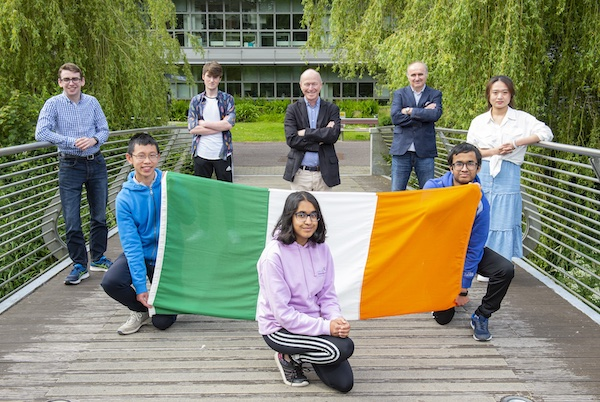
\includegraphics[height=2.035in]{img/olympiad.jpg} &

\includegraphics[height=2.035in]{img/huawei.JPG} \\
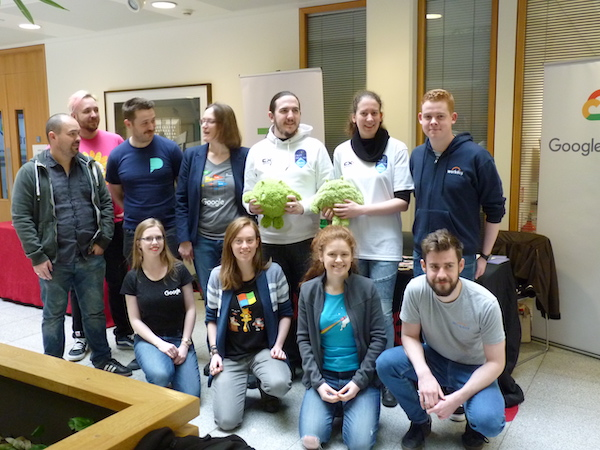
\includegraphics[trim={0 0mm 0 17mm},clip,height=2.035in]{img/google.JPG} &

\includegraphics[height=2.035in]{img/quercus.jpg} \\

\end{tabular}
\end{figure}

\begin{actionblock}{\ksspace{}Appoint mentor for female undergraduates}{edi:coach}
\actappointmentor
\hfill{
    \hypersetup{hidelinks}
    \hyperlink{b4}{\gotoactionsymbol{}}
}
\end{actionblock}

Encouraging female undergraduates to consider a research career 
will be challenging given economic and career 
factors explored in Subsection~\ref{subsec:academic_research}, 
however,  research internship opportunities may help nurture interest (Action~\ref{action:enrich:opportunities}). 

%\todo{JPM changed name of action and preceeding text}
\begin{actionblock}{\ksspace{}Internship opportunities for female undergraduates}{enrich:opportunities}
\actenrichopportunities
\hfill{
    \hypersetup{hidelinks}
    \hyperlink{b5}{\gotoactionsymbol{}}
}
\end{actionblock}

The school aims for gender balanced  representation (both staff and students) at all outreach activities.


\subsection{Provide data for academic and research staff by gender and grade. Analyse and benchmark the career pipeline.}
\label{subsec:academic_research}




Table~\ref{tab:acresstaff} demonstrates that the gender imbalance is stark for both academic and researchers
and at senior levels: there is no female at Senior Postdoctoral 
level or above nor at \ac{SL} level or above. 

Table~\ref{tab:academic_benchmark} compares CSIT's academic
staff profile with that of two peer institutions, \ac{UCD} 
and \ac{TCD}.
The percentage of female academics at CSIT is 9\%, 
compared with 16\% at UCD and 29\% at TCD. 
CSIT has no females at \ac{SL}
level or above, compared with six out of 58 at UCD and five 
out of 59 at TCD. \ac{HESA} data  (2019-20 ICTS) from the 
UK indicates 16\% professors in \ac{CS} are females, 
and 22\% of all research and academic staff excluding professors.

\input{tables2/tab_csit_staff_18nov}

\input{tables2/tab_academic_benchmark_11nov}


CSIT's academic gender profile is largely a reflection of an
uneven recruitment pattern over decades. An expansion of
staff numbers in the 1990s and early 2000s was followed by 
a prolonged  hiring drought, which locked in a historical 
all-male imbalance. Prior to 2017, when our first female colleague 
was recruited, no permanent academic appointment
had been made since 2004.
% Note 2017: AOD, AZ, KJS & PP joined
% 2004: GP joined and none in intervening period.


\pagebreak 
However, since 2017 CSIT has filled 13 academic posts 
(nine male and four female), two of whom (one male, one female)
have since resigned to take up posts in their home country.
%male: KJS, AZ, PP, AA, UR, DP, HC, AV, Harry
%females: AOD, LC,  LM, RM
While this is a step in the right direction, the school realises that 
much work remains to be done to achieve a healthy gender balance, and
%The healthier gender balance evident in recent hires is a positive development and a trend 
will  
adopt gender-positive recruitment measures described in
Section~\ref{sec:academic}
(e.g. Actions~\ref{action:acad:marketing}--\ref{action:acad:cvgaps}).

In the years up to 2027, 12 staff (nine academic, three administrators) are
expected to reach the normal retirement age. Some additional new posts
are also expected based on increasing student numbers. % from new programmes.
This significant number of openings presents an opportunity to approach 
recruitment in a strategic manner, not least to further 
improve gender balance. 



\begin{figbox}{!t}
    \caption[Career pipeline: gender distribution across academic levels of seniority]{Career pipeline: gender distribution across academic levels of seniority, from undergraduate students to Senior Lecturer (SL) and above (2020)}
    \label{fig:pipeline}
    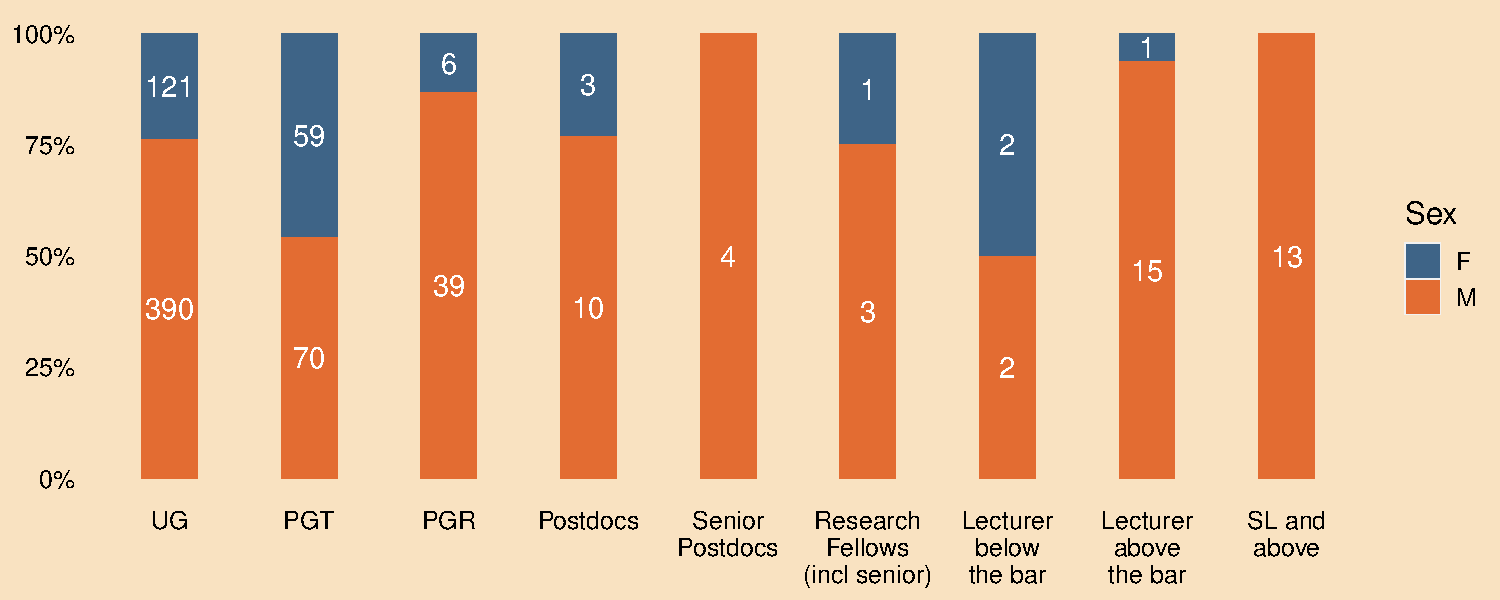
\includegraphics[trim={0 2mm 0 0},clip,width=5.7in]{fig/pipeline.pdf}
\end{figbox}

% \todo{[KJS: Insert figure "The career pipeline"; Tweak to include 
% undergraduates (24\%) and taught postgraduate (46\%) bars.
% See email of 2 Aug 2022.]}

Figure~\ref{fig:pipeline} depicts the career pipeline, showing the
the percentage of females at different career levels from 
undergraduates to professors. 
The ``pipeline'' metaphor can result in an over-focus
on flow from beginning to end, potentially downplaying important 
inward flows at various stages. For example, very few Irish 
undergraduates progress to masters programmes and fewer still
to research studies. 
The healthy numbers and gender balance in our postgraduate programmes 
is largely due to non-EU students. 
%entering at masters or PhD level.
These inward flows are very welcome but camouflage the dearth of female 
undergraduates progressing through PhD and onward to research and
academic careers.

The tapering proportion of females from undergraduates to lecturers to 
senior academics is a global phenomenon in \ac{CS}, but the 
complete lack of females in senior grades at UCC is an outlier even 
within our traditionally male-dominated discipline. 
The greatest choke points appear to be:


\begin{enumerate}[noitemsep]
    \item From undergraduate to research postgraduate
    \item From research roles to academic posts
    \item From Lecturer to \ac{SL} and beyond
\end{enumerate}


Employment prospects for Irish 
computing graduates are buoyant and, unlike other STEM disciplines, 
further postgraduate study is not required for career opportunities
in industry. 

Factors deterring research students and postdocs from pursuing 
academic careers are explored further in 
Section~\ref{sec:academic}. 
Poor PhD stipends (currently at \texteuro{}18,500 p.a.) and low
pay for postdoctoral positions relative to attractive industry salaries 
is one factor. 
Starting salaries on offer to talented 
graduates can be a multiple of the PhD stipend. 
Uncertainties surrounding  securing academic 
positions and promotional opportunities thereafter is another. 


As noted, CSIT has no female academics at \ac{SL}
rank or above, so the Lecturer/\ac{SL} boundary represents
a significant choke point. \label{slboundary}
At UCC academics can attain a senior grade 
either through promotion or direct appointment to an advertised 
position. Promotion criteria and processes at UCC are 
dictated entirely 
by the university and the school has had very limited success with 
promotions over the years.
In the past twenty years, there have been six academic
promotions in all (none since 2014; no females as CSIT did not 
have any female academics until 2017), 
but only three from Lecturer to 
\ac{SL} (most recently in 2008).
In the most recent round (2018-2019), only two 
Lecturers applied for promotion to \ac{SL}; neither was successful (Table~\ref{tab:promotion2sl}).  
If promotions are to contribute to improving gender balance at senior 
levels, 
the school will proactively support colleagues, particularly
females, in navigating UCC's promotion scheme successfully (Action~\ref{action:acad:mentoring}). 

Section~\ref{sec:academic} explores staff experiences
and perception with recruitment and  promotions and proposes
some actions to help improve the gender balance over time. 





\subsection{Provide data for professional, managerial and support staff by gender and grade. Analyse representation, benchmarking where possible.}


% \khcomment{TCD website may allow benchmarking for sysadmin staff}

Table~\ref{tab:pmsstaff} gives an overview of the numbers of \ac{PMS} staff. UCC  classifies
staff in  \ac{CSSS} as ``administrative'' rather than 
``technical.''

\input{tables2/tab_pms_staff_29nov}

Among those in administrative roles in the school's office, 
females predominate; mirroring the situation within the university.
The school's core IT staff are exclusively male. This gender
pattern for administrative and IT roles is replicated among the 
research support staff.
Section~\ref{sec:pms} explores this issue in greater depth 
and presents actions to move the school on a more gender-balanced
trajectory for PMS staff
(e.g. Action
~\ref{action:pms:matchdescription}).

By way of comparison, TCD's webpage currently lists 24 administrative 
staff (21 female, 3 male), nine IT support staff (three female, six
male) and six staff classified as technicians (all male).



\subsection{Provide data on staff on fixed-term contracts, contracts of indefinite duration/permanent contracts, and hourly-paid contracts by gender and staff category. Outline instances where fixed-term and hourly-paid contract types are used. This should include comment on:}
\instr{
\begin{itemize}
    \item whether or not numbers of fixed-term/hourly-paid contracts are representative of a typical year; 
    \item the rationale for the use of short-term contracts;
    \item the extent to which hourly-paid staff contribute to the teaching of core modules and/or services.
\end{itemize}
}

Table~\ref{tab:fthpstaff} summarises CSIT staff by category, contract 
type and gender for 2020.

\input{tables2/tab_fixed_hourly_staff_29nov}

\subsubsection{Comment on whether or not numbers of fixed-term/hourly-paid contracts are representative of a typical year}

The  pattern seen in Table~\ref{tab:fthpstaff}
is  typical of recent years. Hourly-paid contracts are 
never used for research or PMS roles and only rarely for 
academics, as noted below.


\subsubsection{Comment on the rationale for the use of short-term contracts}
\label{rationalecontracts}

Short-term academic contracts (typically one year) are used 
to cover temporary vacancies in permanent posts arising from
maternity cover and retirements. Also posts tied to new programmes are often
sanctioned on a fixed-term basis initially.
%, but the school
%actively lobbies for these to be converted into permanent
%posts.
% DT: Fixed terms 2020: LAB={RM}; LBB = {LM. JQ}
Three of the fixed-term academic shown in 
Table~\ref{tab:fthpstaff} have subsequently received 
permanent positions, two of whom are female.



Research activity is wholly dependent on the flow of research 
funding which is inherently impermanent and so all researchers 
are on fixed-term contracts. A number of those in research 
administration or research IT support roles have core
permanent/\ac{CID} positions, some appointed to a 
higher-grade from research funds.

\subsubsection{Comment on the extent to which hourly-paid staff contribute to the teaching of core modules and/or services}

Hourly paid staff are mainly students
employed on a part-time basis as laboratory demonstrators or tutors for
undergraduate modules. The amount of such work varies by year; 
in 2019-20, for example, we had 65 hourly paid staff: 54 male and 11 female (17\%), which is below the percentage of 
female undergraduate and taught postgraduates.

A handful of modules (3\%) are covered by hourly-paid part-time lecturers---generally postdocs seeking teaching experience.







\newpage
\newpage 
\section{Embedding policy, practice and supports to advance academic and research careers}
\label{sec:academic}



\subsection{Reflecting on recruitment practices in the department}


\instr{

\begin{prompt}
\setlength\tabcolsep{6pt} 
\begin{tabu} to \textwidth {@{} X[9] X X }
     \multirow{2}{=}{Recruitment to academic and research posts in the department adheres to institutional policy on recruitment, which includes gender-balanced panels and training for assessors } 
     & \textbf{Yes} & \textbf{No}  \\
     &  \Square & \XBox  \\[.1in] 

\end{tabu}
\setlength\tabcolsep{0pt} 
\end{prompt}
If you answered `no', please comment.
}

The policies that apply to gender-balanced panels and training for selection committee members for academic posts, do not apply to recruiting researchers.  Table~\ref{tab:committee:gender:balance:research} shows that in the previous 3 years only 19\%, on average,  of recruitment committee members for research positions were female, many were entirely male. To address the training requirements and gender-balanced panels, the school will require all committee members to undergo training, e.g., recruitment and selection training (Action~\ref{action:acad:recruittraining}).


\input{tables2/tab_committee_gender_balance}


\begin{actionblock}{\ksspace{}School policy on research recruitment}{acad:recruittraining}
\actrecruitmenttraining
\hfill{
    \hypersetup{hidelinks}
    \hyperlink{c7}{\gotoactionsymbol{}}
}
\end{actionblock}




Table~\ref{tab:selection:acad} shows that recruitment for academic posts;  over 70\% of the selection committees had more than 40\% female representation.

\input{tables2/tab_selection_acad}





\subsection{Provide three years of data on application, shortlist, and appointment rates for recruitment by gender and grade. Where data suggests opportunity for improvement, comment and reflect. Include any other relevant information relating to recruitment processes and practice for academic and research posts in the department. }

Academic recruitment is centrally managed by \ac{HR}. There were nine academic appointments from 2017 to 2019 (Table~\ref{tab:equality:recruitment:academic}).

There were significantly fewer female applicants, particularly for the Professorship in 2017/18. 
No female applicant was appointed in 2017/18, however, in 2018/19,  3 of the 5 appointees were female. 

\input{tables2/tab_recruitment_acad}

The school is committed to addressing the gender imbalance across academic staff (Table~\ref{tab:acresstaff}), in particular at \ac{SL} level and above.
It took part in the \ac{SALI} Chair initiative in 2019 and in 2020 for establishing a female professorship for the school. Unfortunately, the school's bid was unsuccessful. In 2021, the school advertised a Professorship in Human Centred Computing. Of the five shortlisted applicants, two were women and both were deemed appointable. Both declined; one citing the high teaching workload as unattractive (Action~\ref{action:acad:transparentworkload}).

While exploring how to increase the number of female applicants for academic posts, it was suggested that the language used in advertisements might be inadvertantly discouraging such applicants:

\begin{myquote}
``... can write a job advert in a way that discourages women from applying – it's the language you use ...''
\end{myquote}

Consequently, the school will adopt gender neutral language and seek to use gender decoders when creating advertisements for academic and research positions (Action~\ref{action:acad:marketing}). Furthermore,  we will actively target female applicants for all posts (Action~\ref{action:acad:femaleonly}).


\begin{actionblock}{\ksspace{}Improve advertising text}{acad:marketing}
\actimproveadvertisingtext
\hfill{
    \hypersetup{hidelinks}
    \hyperlink{c2}{\gotoactionsymbol{}}
}
\end{actionblock}


\begin{actionblock}{\ksspace{}Target suitable female academics and researchers}{acad:femaleonly}
\acttargetfemales
\hfill{
    \hypersetup{hidelinks}
    \hyperlink{c1}{\gotoactionsymbol{}}
}
\end{actionblock}

In the period from 2017 to 2020, 21\% of research appointments in CSIT were female. This is similar to the proportion of female PhD holders in Computer Science, globally. 

The survey revealed that researchers remained unconvinced of adequate training and mentoring opportunities towards promotion (Figure~\ref{fig:research:access}); for researchers, promotion implies either a higher researcher grade (e.g. Senior Research Fellow), or a permanent academic position.

\begin{figbox}{!t}
\caption{Access to training and mentoring needed for promotion (Researchers)}
\label{fig:research:access}
\footnotesize 
    \begin{tabular}{P{5.6cm}p{8cm}}
    \addlinespace 
    I have access to the training and mentoring I need to help me meet the criteria for promotion or to improve my success at promotion & 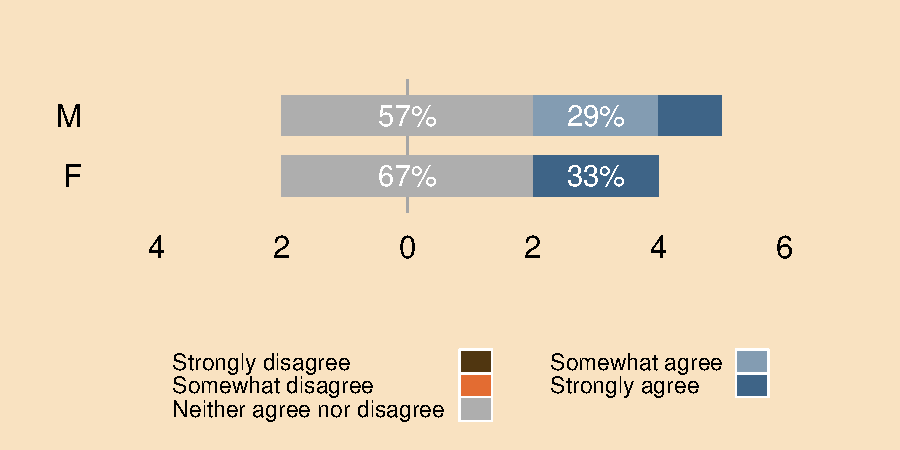
\includegraphics[align=t,trim={0 20mm 15mm 16mm},clip,width=8cm]{fig/careerdev/dirk_accessR.pdf}\\
    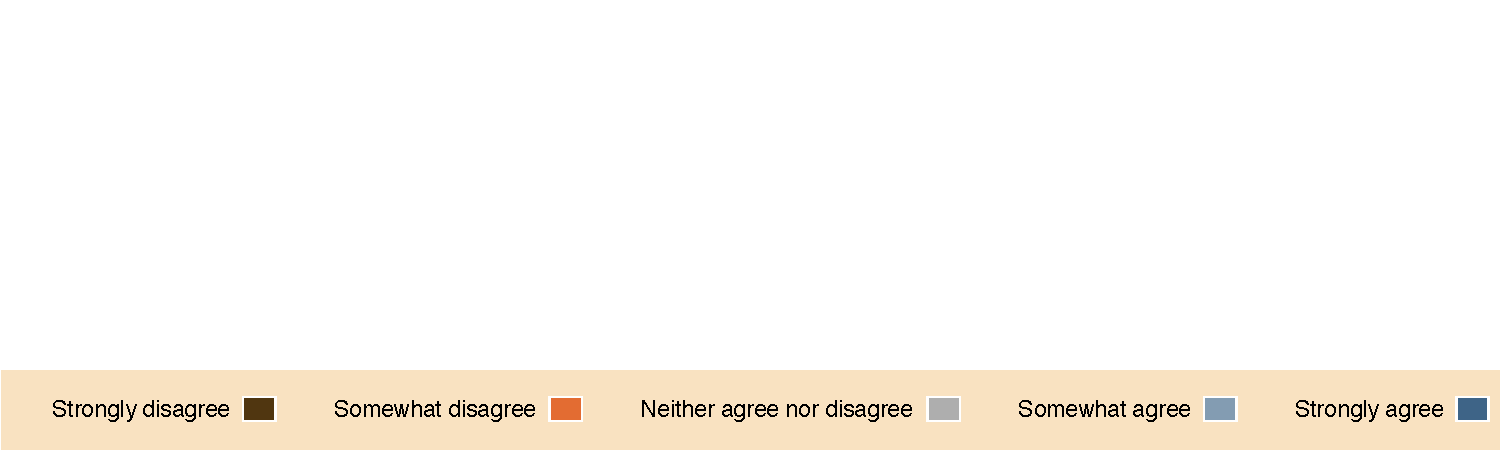
\includegraphics[trim={6mm 0 0 0},clip,width=14.5cm]{fig/legend5col.pdf}
    \end{tabular}
\end{figbox}




In the focus group, researchers requested help be made available with personal development plans (Action~\ref{action:acad:mentorresearchers}).



\begin{actionblock}{\ksspace{}Support researchers with personal development plan}{acad:mentorresearchers}
\actmentorresearchers
\hfill{
    \hypersetup{hidelinks}
    \hyperlink{c4}{\gotoactionsymbol{}}
}
\end{actionblock}

The staff focus group highlighted the need to allow applicants to account for gaps in their CVs --- particularly related to maternity leave and caring responsibilities. 

\begin{myquote}
``There isn’t a guideline, ... that says, look if you have had a family break of any kind, … you have this opportunity to describe it … so that if you have gaps in your CV, you can explain them, because gaps in a CV are a red flag if they're not explained.''
\end{myquote}


Consequently, the school will accept `Leave Statements' as part of its recruitment process (Action~\ref{action:acad:cvgaps}).


\begin{actionblock}{\ksspace{}Consider leave statements}{acad:cvgaps}
\actincludeleavestatement 
\hfill{
    \hypersetup{hidelinks}
    \hyperlink{c6}{\gotoactionsymbol{}}
}
\end{actionblock}


\subsection{Reflecting on academic promotion in your institution, answer the following: }

\instr{
\begin{prompt}
\setlength\tabcolsep{6pt} 
\begin{tabu} to \textwidth {@{} X[8] X X X }
     \multirow{2}{=}{Academic promotion processes, including eligibility criteria, are managed centrally by the institution} & \textbf{Yes} & \textbf{No}  & \textbf{N/A}\\
     &  \XBox & \Square  & \Square \\ 
\end{tabu}
\setlength\tabcolsep{0pt} 
\end{prompt}
}

\instr{If you answered ‘no’, please comment on the department’s role in academic promotions processes. If you answered ‘not applicable’, as prescribed promotion pathways are not in place in your institution, provide comment and reflection on alternative routes for academic career progression.}

\subsection{Provide three years of data on application and success rates for promotion by gender and grade and present results from staff consultation by gender. Where data suggests opportunity for improvement, comment and reflect}

As discussed on Page~\pageref{slboundary}, only one call for promotion (2018/19) was issued from 2017 to 2019, resulting in no successful candidates (Table~\ref{tab:promotion2sl}). 


\input{tables2/tab_promotion2sl}



Both the staff survey and focus groups revealed that staff are unhappy with the lack of promotion opportunities. 
Many respondents felt that the promotion process and criteria are neither transparent nor fair.  

\begin{figbox}{!ht}
\caption{Access to training and mentoring needed for promotion (Academics)}
\label{fig:academic:access}
\footnotesize
    \begin{tabular}{P{5.6cm}p{8cm}}
    \addlinespace 
    I have access to the training and mentoring I need to help me meet the criteria for promotion or to improve my success at promotion & 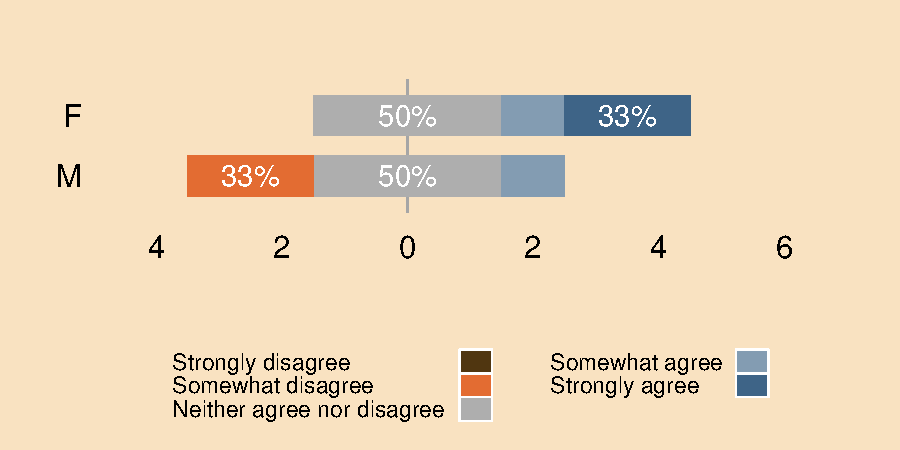
\includegraphics[align=t,trim={0 20mm 15mm 16mm},clip,width=8cm]{fig/careerdev/dirk_accessA.pdf}\\
    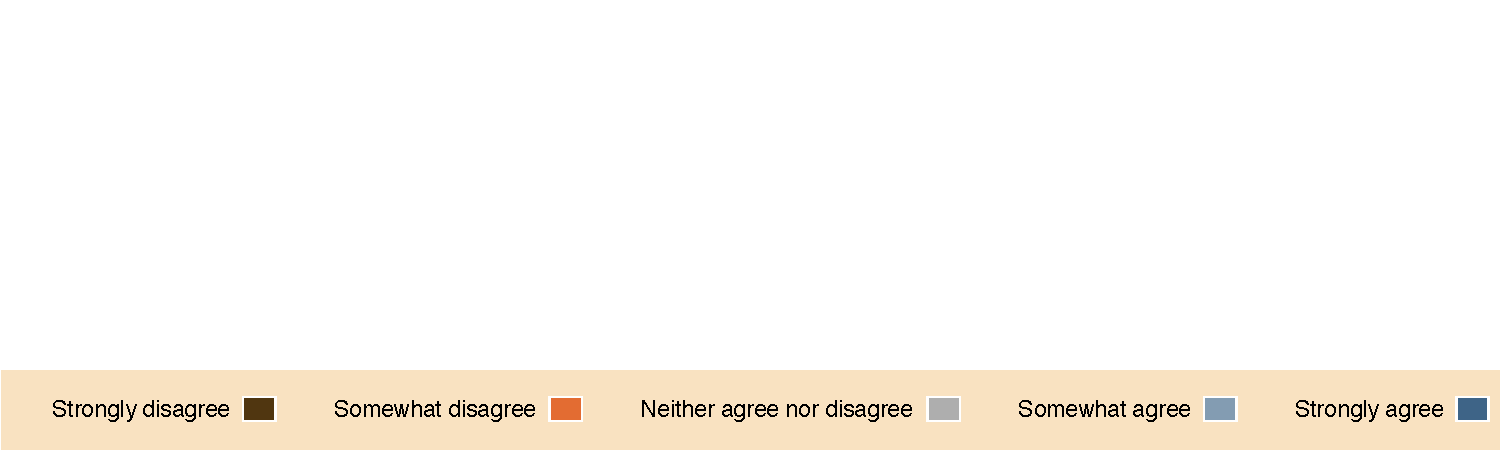
\includegraphics[trim={6mm 0 0 0},clip,width=14.5cm]{fig/legend5col.pdf}\\
    \end{tabular}
\end{figbox}



\begin{myquote}
``There is no promotion scheme... It seems to be an impossible process to ... become a professor in UCC. I’ve kind of given up hope, to be honest.''
\end{myquote}

\begin{myquote}
``In essence, there is no realistic prospect of promotion whatsoever... ''
\end{myquote}


\begin{myquote}
``I don’t think I’ll ever get a [more senior] position, ... I’m never going to get one of those because they do not align with my area of expertise.''
\end{myquote}

Since the consultation, academic progression and promotion schemes underwent a review in 2022. A call for progression across the merit bar opened in 2022. Calls for promotion to SL will open in early 2023 and to Professor (Scale 2) in 2024.

It was decided that a mentoring scheme to support colleagues seeking promotion would benefit all staff and would encourage female staff, in particular, to engage with the system (Action~\ref{action:acad:mentoring}). 



\begin{actionblock}{\ksspace{}Academic mentoring scheme}{acad:mentoring}
\actmentorpromotion
\hfill{
    \hypersetup{hidelinks}
    \hyperlink{c10}{\gotoactionsymbol{}}
}
\end{actionblock}




%\input{tables2/tab_recruitment_acad}


\subsection{Reflecting on opportunities for staff development reviews, answer the following:}\label{sec:2e}

\instr{
\begin{prompt}
\setlength\tabcolsep{6pt} 
\begin{tabu} to \textwidth {@{} X[8] X X @{}}
     \multirow{2}{=}{The institution operates a development review process, or equivalent, for academic and research staff} & \textbf{Yes} & \textbf{No}  \\
     &  \XBox & \Square   \\ 
\end{tabu}
\setlength\tabcolsep{0pt} 
\end{prompt}
}

\instr{
If you answered ‘yes’, comment and reflect on the implementation of this institution-level process in the department. This should include: 
\begin{itemize}
\item	data on uptake by gender;
\item	results from staff consultation presented by gender;
\item	information on any additional department-level opportunities for staff to discuss professional development. 
\end{itemize}

\noindent If you answered ‘no’, provide detail on department-level opportunities for staff to discuss professional development, including data on uptake by gender and results from staff consultation presented by gender. 
}\label{acad:pdrs}



UCC operates a Performance Development and Review System (\ac{PDRS}), which applies to all staff, except for those with less than 50\% FTE, less than a year left on a contract, staff on probation, on long term sick leave, or within two years of retirement. As part of the process, staff can discuss their development needs with their line manager. The process did not operate from 2017 to 2020; it was scheduled to restart in 2019, but this was further postponed due to Covid-19 restrictions in 2019 and 2020. 


\begin{figbox}[10cm]{!b}
    \caption{Awareness of the Performance Development Review System}
     %trim={<left> <lower> <right> <upper>}
    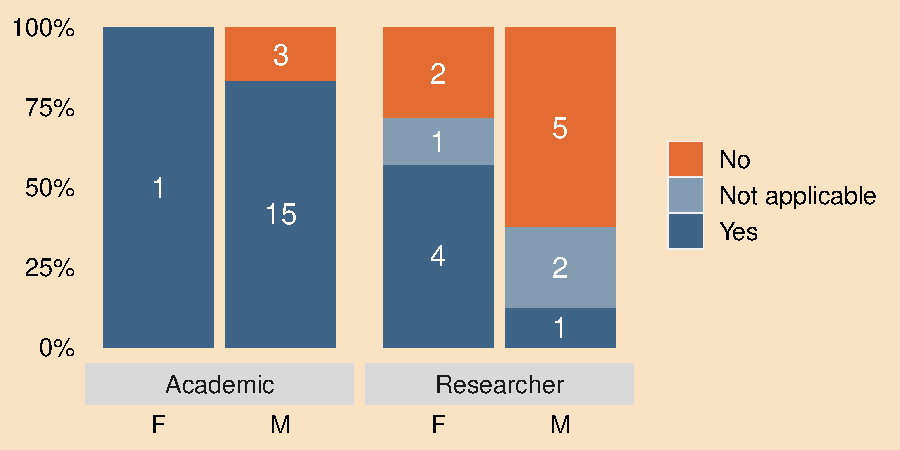
\includegraphics[trim={0 0 0 0},clip,width=9cm]{fig/awareness.pdf}
    \label{fig:awareness}
\end{figbox}


The staff survey revealed that the majority of academic staff were aware of the PDRS process (100\% female, 80\% male). 
However, the majority of research staff were unaware of the process (Figure~\ref{fig:awareness}). 
The survey data suggests that the female academic staff respondent was satisfied with the opportunity to engage with the 
\ac{HOS} on performance and development, approximately 15\% of male academic staff are not satisfied (neutral to or disagree with) with those opportunities (Figure~\ref{fig:acadcareerdev}). 



\begin{figbox}{!t}
    \sffamily 
    \footnotesize 
    \raggedright 
    \caption{Academic career development opportunities}        
    
    \begin{tabular}{P{5cm}p{9cm}}
    \addlinespace 
    
    I am satisfied with the opportunities I have to discuss my career progress with my line-manager &
    % left down right up
    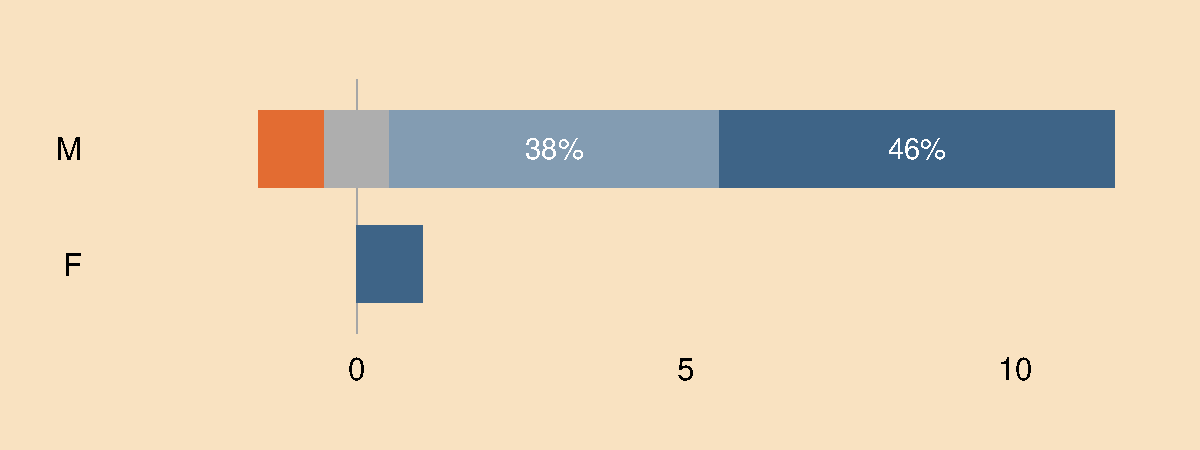
\includegraphics[align=t,trim={0 4mm 10mm 17mm} ,clip,width=9cm]{fig/careerdev/dirk_career.pdf}\\

\hdashline

    I am satisfied with the opportunities I have to discuss promotion opportunities with my line-manager
    &
    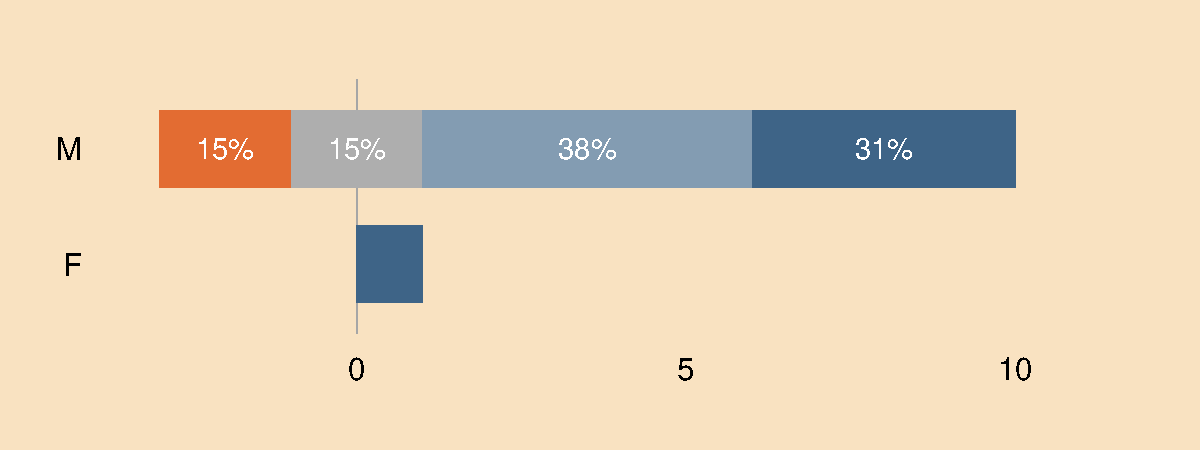
\includegraphics[align=t,trim={0 4mm 10mm 17mm} ,clip,width=9cm]{fig/careerdev/dirk_promotion.pdf}\\
   
\hdashline

    I am satisfied with the opportunities I have to discuss my work-load with my line manager
    &
    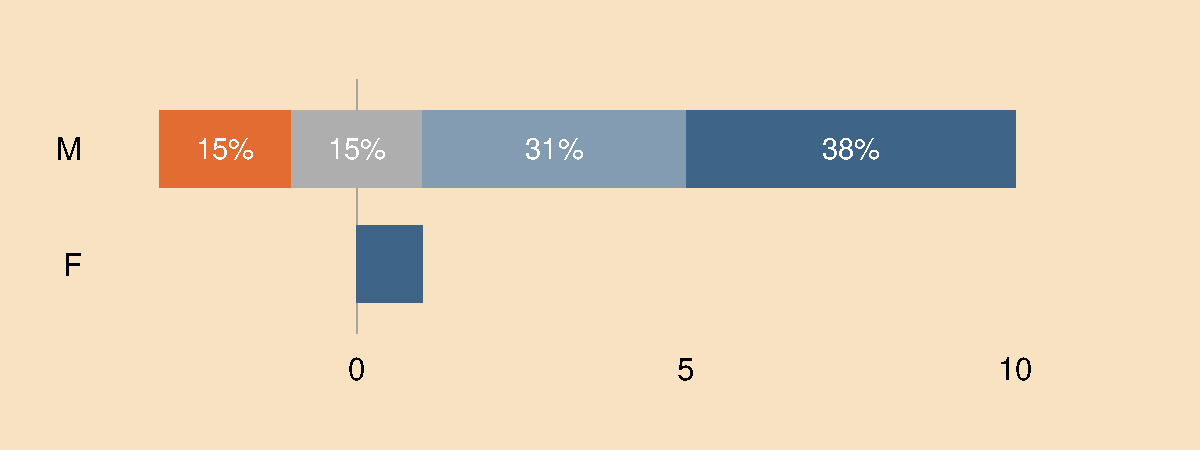
\includegraphics[align=t,trim={0 4mm 10mm 17mm} ,clip,width=9cm]{fig/careerdev/dirk_workload.pdf}\\

\hdashline

    I am satisfied with the opportunities I have to discuss my work objectives with my line manager
    &
    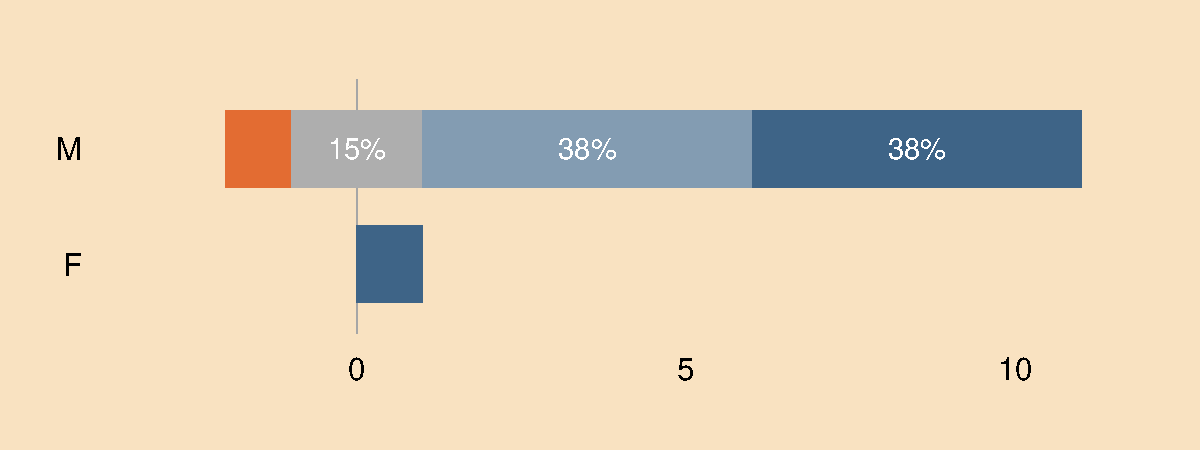
\includegraphics[align=t,trim={0 4mm 10mm 17mm} ,clip,width=9cm]{fig/careerdev/dirk_objectives.pdf}\\

    %% Legend
    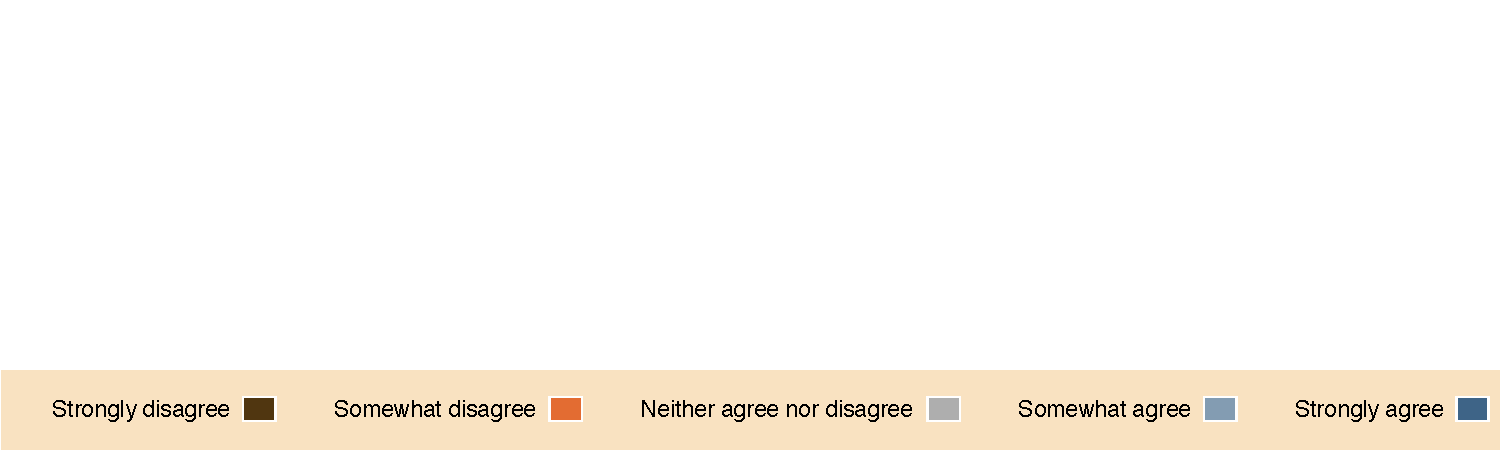
\includegraphics[trim={6mm 0 0 0},clip,width=14.5cm]{fig/legend5col.pdf}\\

    \end{tabular}
    \label{fig:acadcareerdev}
\end{figbox}


\pagebreak
Comments on the \ac{PDRS} process during the academic staff focus group were mixed:

\begin{myquote}
``The only conversations that I have with a line manager or head of department would be [about teaching schedules] ...''
\end{myquote}

\begin{myquote}
`` ... he was very helpful. He tried to map out where are your weaknesses? [and supported me to develop in those areas]''
\end{myquote}



It is hoped that Action~\ref{action:acad:pdrs} would address these concerns.
% Figure with awareness of PDRS process.


\begin{actionblock}{\ksspace{}Restart PDRS process}{acad:pdrs}
\actrestartpdrs
\hfill{
    \hypersetup{hidelinks}
    \hyperlink{c13}{\gotoactionsymbol{}}
}
\end{actionblock}

Researcher feedback from the staff survey and focus groups was mixed (Figure~\ref{fig:research:career:planning}). The survey data indicated that approximately 70\% of respondents never had a `development needs' meeting with their line manager (PI). Approximately 90\%  have no personal development plan, 90\% have no training objectives and 67\% of those who do, consider that they are not meeting their training objectives.
Nevertheless, respondents commended the development opportunities available within UCC and felt supported by the school to avail of those opportunities (Figure~\ref{fig:research:career:development}). 


  
\begin{figbox}{!hb}
    \caption{Support for researcher career planning}
    \label{fig:research:career:planning}

    \sffamily 
    \footnotesize 
    \raggedright 
    \begin{tabular}{P{5cm}!
                    {\quad}
                    p{9cm}}
    \addlinespace
    I am satisfied with the opportunities I have to discuss career progress with my PI & 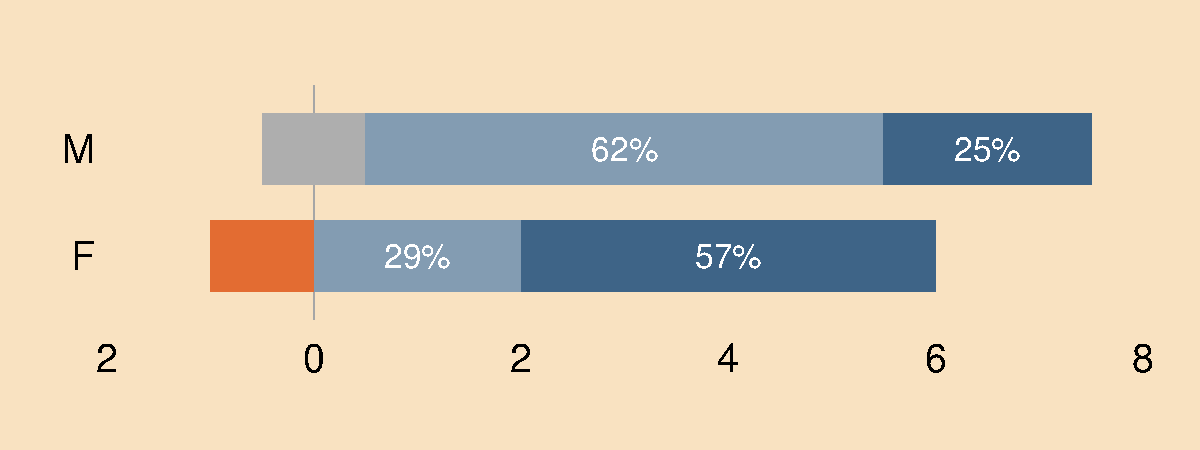
\includegraphics[align=t,trim={0 4mm 7mm 17mm},clip,width=8cm]{fig/careerplan/dirk_carprogress.pdf}\\

\hdashline
    I am satisfied with the opportunities I have to discuss promotion opportunities with my PI & 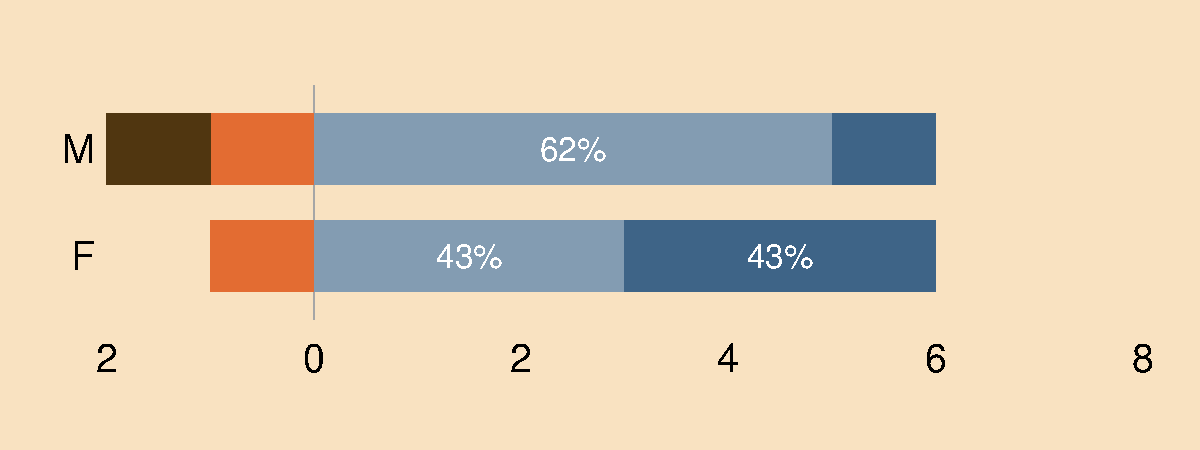
\includegraphics[align=t, trim={0 4mm 7mm 17mm}, clip, width=8cm]{fig/careerplan/dirk_carpromotion.pdf}\\
\hdashline
    I discuss training and mentoring opportunities with my PI &
    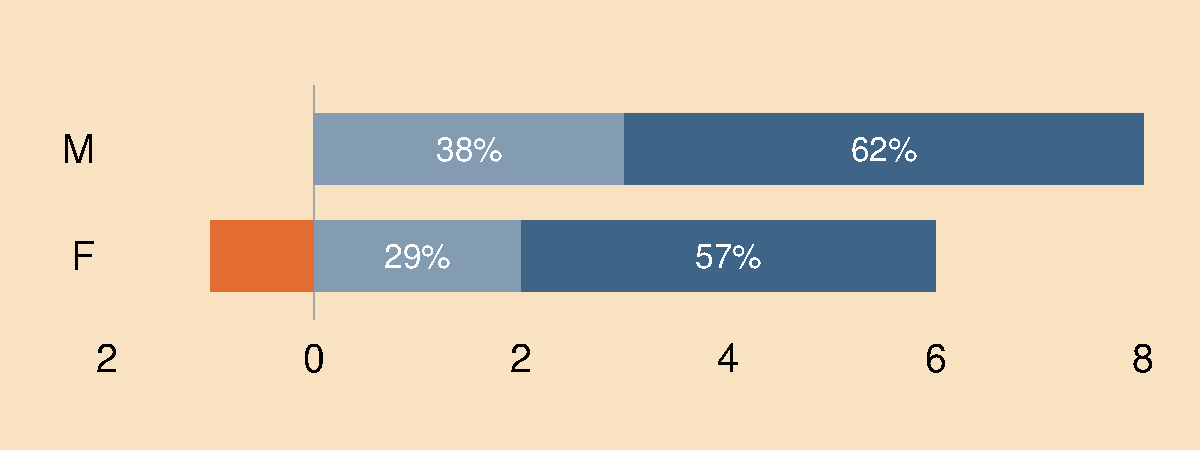
\includegraphics[align=t, trim={0 4mm 7mm 17mm}, clip, width=8cm]{fig/careerplan/dirk_carmentoring.pdf}\\

    %% Legend.
    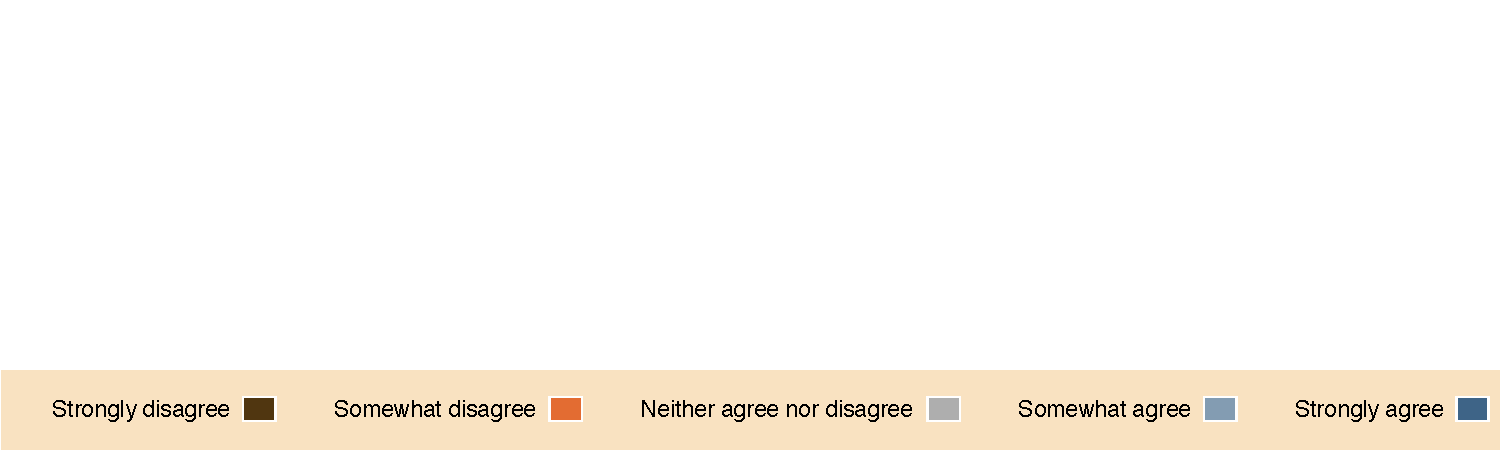
\includegraphics[trim={6mm 0 0 0},clip,width=14.5cm]{fig/legend5col.pdf}\\
    
    \end{tabular}        
\end{figbox}


Overall, evidence suggests that many academic and research staff are unhappy with career development opportunities and supports (Action~\ref{action:acad:pdrs}). 


\begin{figbox}{!t}
    \caption{Research staff career development}
    \label{fig:research:career:development}
     %trim={<left> <lower> <right> <upper>}

    \sffamily
    \raggedright
    \footnotesize
    \begin{tabular}{P{5.5cm}p{8cm}}
    \addlinespace
    Have you met with your PI to prepare a Professional Development Plan?  & 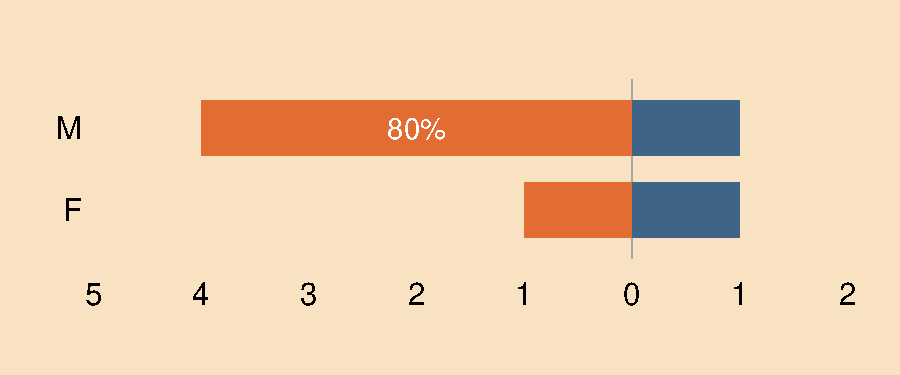
\includegraphics[align=t,trim={0 0 0 16mm},clip,width=8cm]{fig/rescareerdev/dirk_havemet.pdf}\\
\hdashline
    Do you have a current professional development plan? & 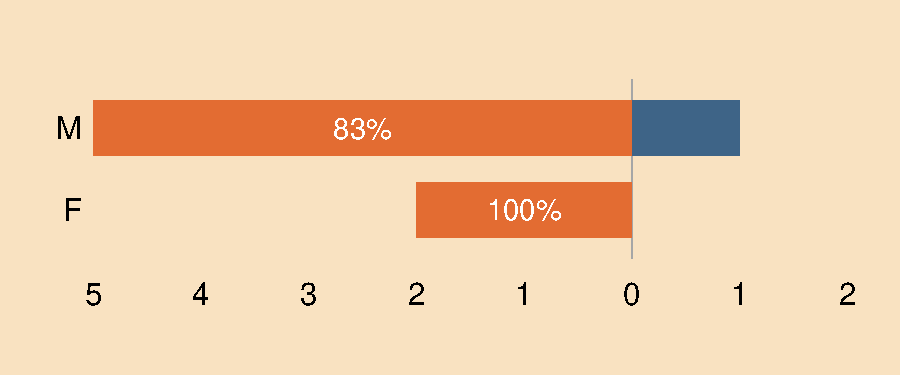
\includegraphics[align=t,trim={0 0 0 16mm},clip,width=8cm]{fig/rescareerdev/dirk_haveplan.pdf}\\
\hdashline
    Does your Professional Development Plan identify specific training objectives? & 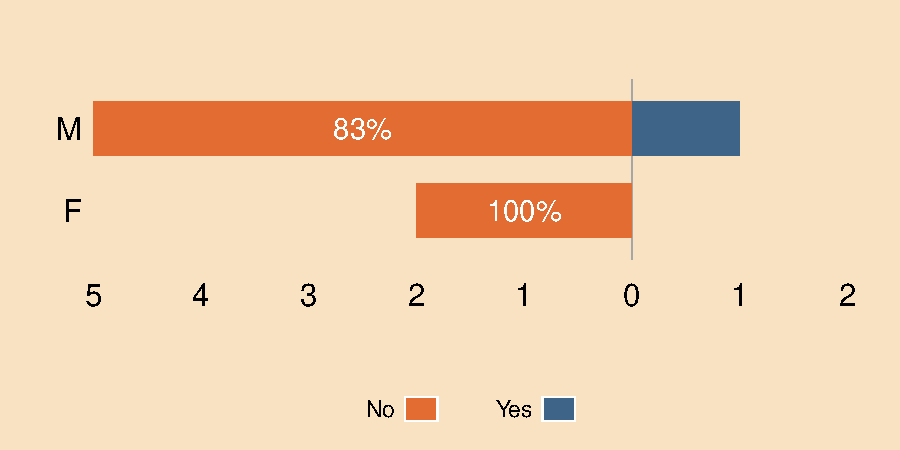
\includegraphics[align=t,trim={0 0 0 16mm},clip,width=8cm]{fig/rescareerdev/dirk_specify.pdf}\\
    
    \end{tabular}
    
\end{figbox}




\subsection{Comment and reflect on department engagement with institution-level supports for academic and research staff career progression as well as any department-level support available. This should include results from staff consultation presented by gender and may include, but is not limited to, support given to staff to:}\label{sec:2f}
\instr{
\begin{itemize}
\item	apply for research funding;
\item	develop excellence in teaching and learning.
\end{itemize}
}

\subsubsection{Comments and Reflections on Institution-level Supports for Career Progression} 

UCC provides training and development programmes for academic and research staff. These include personal and professional development, management and leadership development, and staff wellbeing, which are coordinated by HR, the \ac{OVPRI}, and the Office of the VP for Teaching and Learning. 
Table~\ref{tab:training:academic} 
shows the uptake of development opportunities by academic staff in the report period.  

\input{tables2/tab_training_acad}


Irish universities consider postdoctoral staff as `research trainees.' UCC provides many training and development opportunities via its PostDoc Development Hub.\footnote{\url{https://www.ucc.ie/en/hr/research/devhub/}} 
Table~\ref{tab:training:postdoc} shows these courses and their uptake in the report period. The data do not indicate how many researchers availed of these, but the uptake is limited, particularly among male researchers. 
 

\newpage 
\input{tables2/tab_training_postdoc_mdframed}

There was a marked difference between female and male staff taking up training opportunities (Figure~\ref{fig:training}). The female respondant was happy with the training opportunities and their relevance, the male staff were less happy. They had a lack of awareness, relevance and availability of training opportunities, a perceived lack of support by line manager to participate in training, a perceived lack of opportunity to attend conferences, and some reported a lack of opportunity to present their work to school peers.

\begin{figbox}{!h}
    \caption{Training awareness}
    \label{fig:training}
    % left lower right upper
    

    \sffamily
    \raggedright
    \footnotesize
    \begin{tabular}{P{3.5cm}p{10cm}}
    \addlinespace
    
    I am aware of training opportunities available to me (Academics) &   
    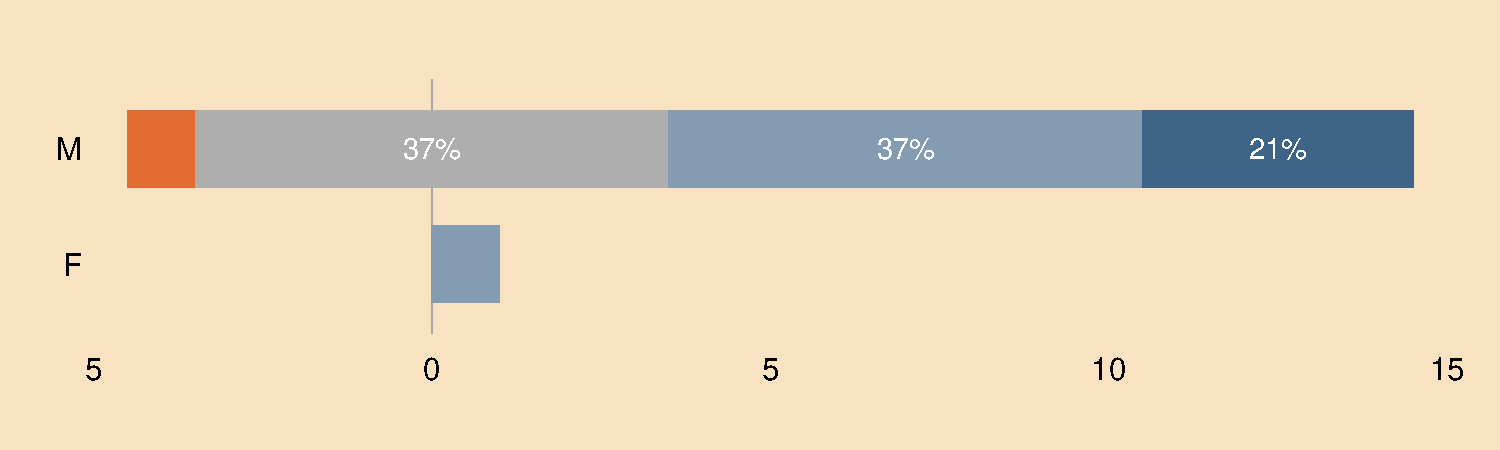
\includegraphics[align=t,trim={0mm 16mm 0 16mm},clip,width=11cm]{fig/training/dirk_trainingV2aA.pdf}\\
    As above, for Researchers & 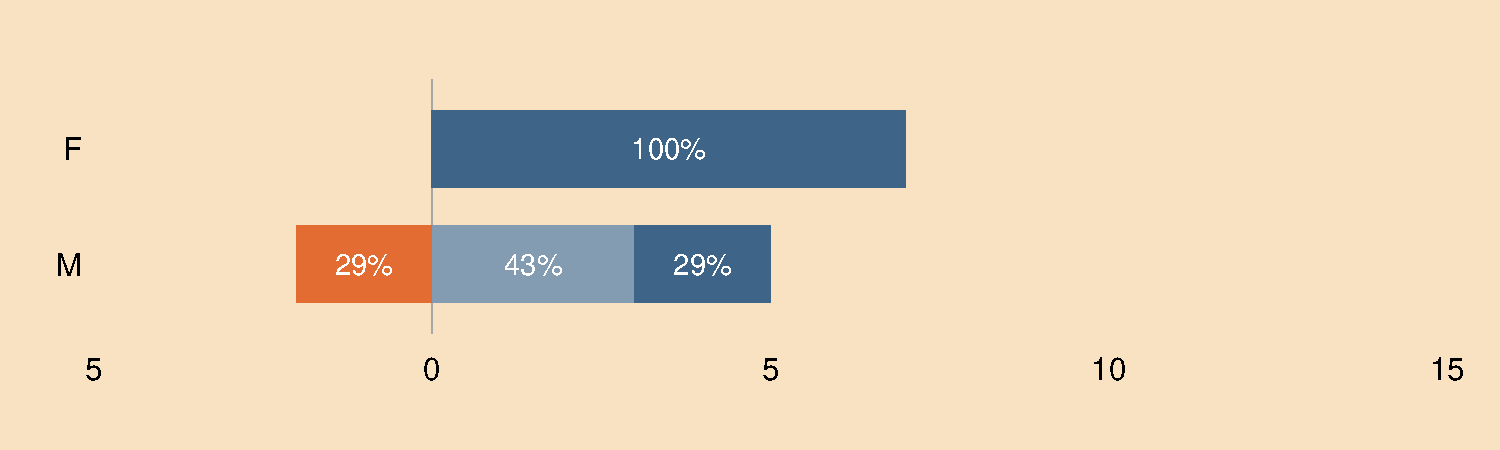
\includegraphics[align=t,trim={0mm 4mm 0 18mm},clip,width=11cm]{fig/training/dirk_trainingV2aR.pdf}\\
    

    \hdashline
    The relevance of the training opportunities is clear to me (Academics) &   
    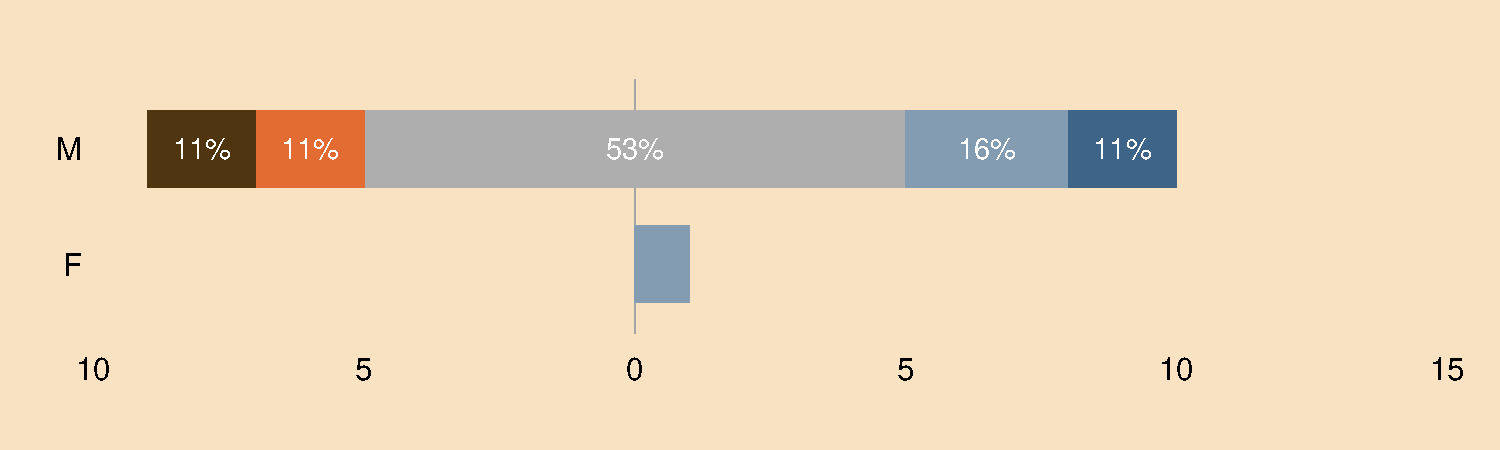
\includegraphics[align=t,trim={0mm 16mm 0 16mm},clip,width=11cm]{fig/training/dirk_trainingV2bA.pdf}\\

    As above, for Researchers &   
    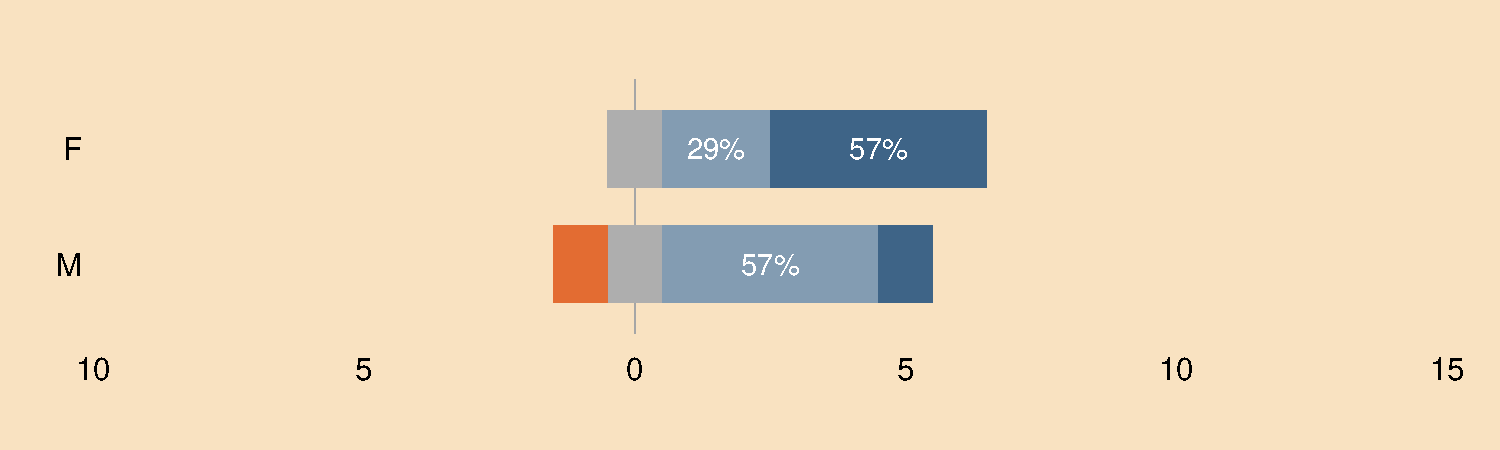
\includegraphics[align=t,trim={0mm 4mm 0 18mm},clip,width=11cm]{fig/training/dirk_trainingV2bR.pdf}\\
    
    \hdashline
    I am satisfied with the training opportunities available to me (Academics) &   
    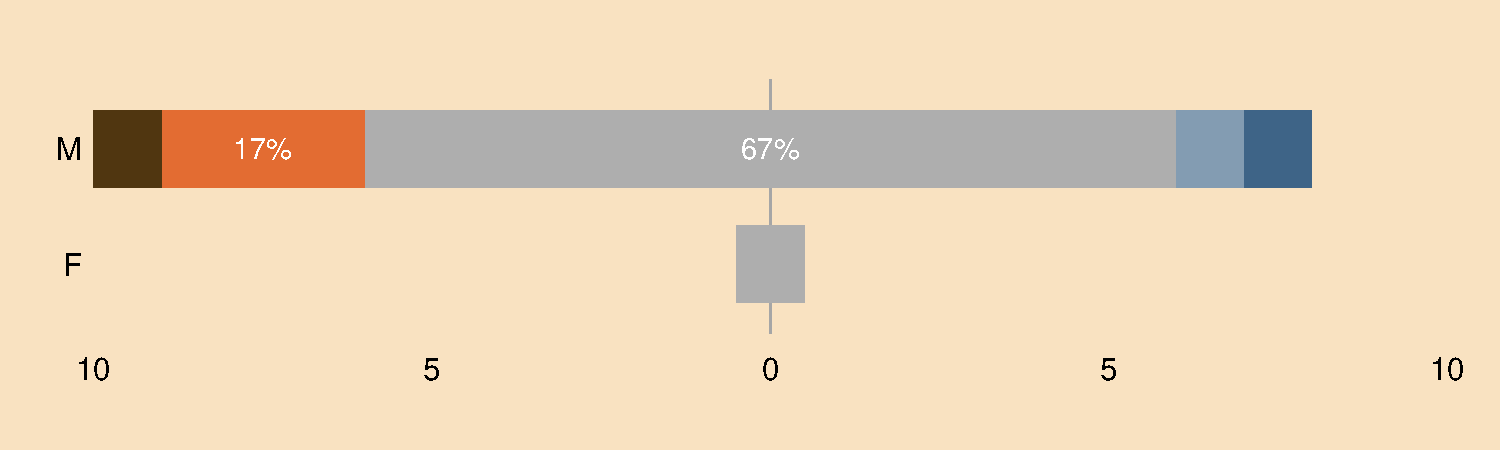
\includegraphics[align=t,trim={0mm 16mm 0 16mm},clip,width=11cm]{fig/training/dirk_trainingV2cA.pdf}\\

    As above, for Researchers &   
    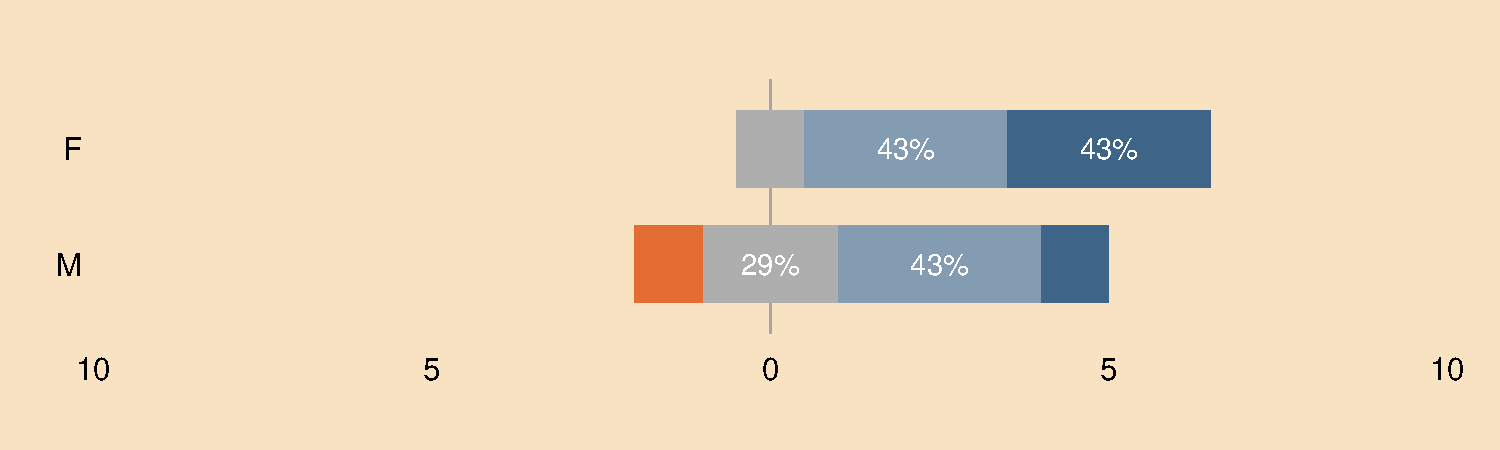
\includegraphics[align=t,trim={0mm 4mm 0 18mm},clip,width=11cm]{fig/training/dirk_trainingV2cR.pdf}\\


    % %% Legend
    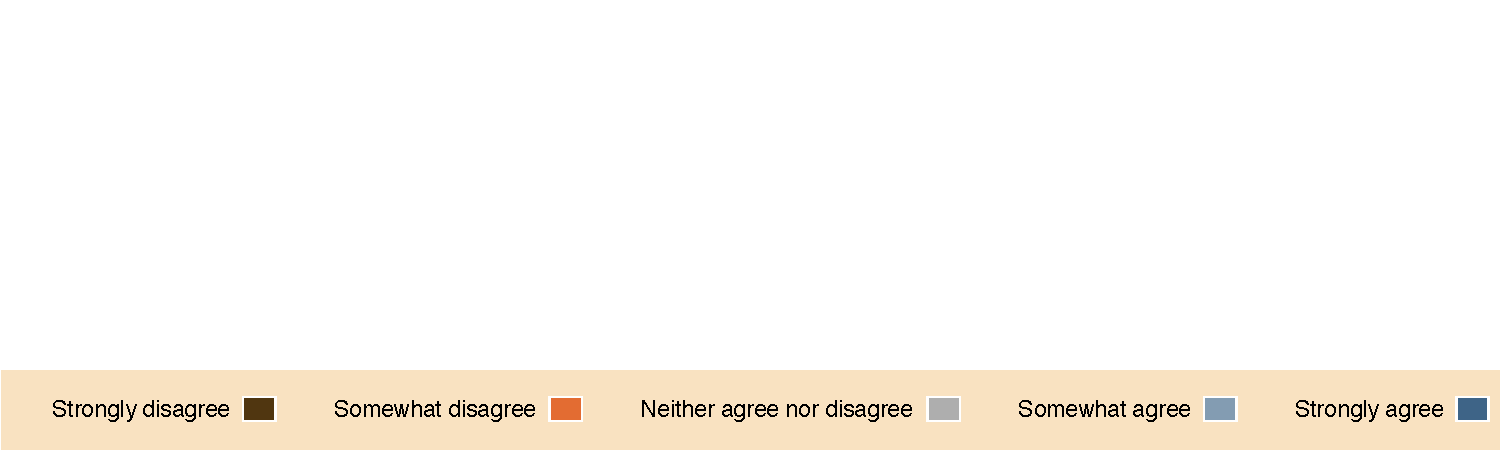
\includegraphics[trim={6mm 0 0 0},clip,width=14.5cm]{fig/legend5col.pdf}\\
    
     \end{tabular}
    
\end{figbox}



Research staff have a more positive view and more balance can be seen between male and female respondents (Figure~\ref{fig:training}). 
A desire was expressed for better communication on training and development opportunities:

\begin{myquote}
``It's important to keep training to keep up to date. I'd like more open discussion around training needs and requirements.''
\end{myquote}

\begin{myquote}
“Unfortunately, I have never heard or seen any email where funding for training has been circulated or promoted.''
\end{myquote}

Academic staff in the focus group were satisified with the school supports and with training offered centrally, but they perceived the uptake to be low. They suggested that the school should echo these opportunities to the staff:

\begin{myquote}
``Those kind of courses [like CIRTL – Centre for Integration of Research, Teaching, and Learning] should be advertised by the department … courses that we can improve … project management skills, soft skills, hard skills … I think that would really benefit us going forward.''
\end{myquote}

Research staff in the focus group would like to see more support for research staff development at school level. Currently, support for career development mainly comes from their respective research centres and groups. 
Consequently, not all researchers may have the same opportunities; researchers who were not part of a centre or large group reported being isolated. As mentioned, the PDRS will restart (Action~\ref{action:acad:pdrs}), which will incorporate career development for research staff, and the PDRS will also serve as a mechanism to make staff aware of training opportunities. 





\subsubsection{Support for Research Funding Applications}

Figure~\ref{fig:fundingsupport} presents results regarding perceived importance, opportunities, and support for research funding, disaggregated by staff category (academic, research) and gender. 
Overall, staff perceived opportunities to apply for research funding is important to their professional development.
The data revealed a number of issues.

\input{2_2_fig226.tex}

While available opportunities to apply for funding were mostly satisfactory for both academics and researchers, a number of academics and researchers were dissatisfied. Further, most respondents also were satisfied with the support available within the school to apply for funding, a small number respondents were not. 
Less satisfied were a number of male academics with the support provided by the university, for example through the \ac{OVPRI} and the college. 
Finally, there is some room for improvement to provide support to those whose funding applications were not successful. While several respondents answered neutral (neither agree/disagree), male academics in particular found this lacking.








Success in attracting research funding is a key factor in academic career progression for both researchers and academics, and in response the school will create a programme to support staff before, during, and after the funding application process (Action~\ref{action:acad:supportfunding}). 


\begin{actionblock}{\ksspace{}Research funding support programme}{acad:supportfunding}
\actsupportprogramme
\hfill{
    \hypersetup{hidelinks}
    \hyperlink{c16}{\gotoactionsymbol{}}
}
\end{actionblock}



\subsubsection{Support for Development of Excellence in Teaching and Learning}

A qualification in teaching and learning is essential for promotion from Lecturer to Senior Lecturer so the school encourages all academic staff to avail of the courses offered by \ac{CIRTL}.

Academic survey respondents  were broadly satisfied with access to and support for equipment and digital tools, for teaching and research. The IT support group are held in high esteem. 

Research staff focus group respondents would like to have more clarity on opportunities to participate in tutoring, lecturing and other academic duties (Action~\ref{action:acad:handbook}).

\begin{actionblock}{\ksspace{}Opportunities for research staff to engage in school academic activities}{acad:handbook}
\acthandbook
\hfill{
    \hypersetup{hidelinks}
    \hyperlink{cxx1}{\gotoactionsymbol{}}
}
\end{actionblock}


\subsection{Comment and reflect on how workload is allocated and managed in the department (e.g. via a workload allocation model). This should include information on how the breadth of academic and research roles and responsibilities are captured in workload planning and allocation and results from staff consultation presented by gender.}\label{sub:workload}


\subsubsection{Workload Model and Allocation}

Academic staff workload includes teaching, research, and administration. Research staff primarily conduct research, but may also be asked to undertake light administrative tasks and/or contribute to teaching.
Research workload for academic staff is somewhat self-allocated and varies by staff member.
Workload is allocated by the \ac{HOS} 
to cover core teaching and administrative duties. 
New staff are assigned a reduced teaching load for their first year to enable them to develop their research agenda.
There is very limited recognition of research workload in the school's workload distribution scheme. This can result in a higher workload for research active staff. 

Workload allocation for research staff depends on their line manager and on their ambition.

\clearpage 
\input{2_2_fig227.tex}



\begin{figbox}{!t}
    \caption{Perceived changes to workload since Covid-19}
    % left lower right upper
    
    \label{fig:workloadchange}

    \sffamily
    \footnotesize
    \raggedright
    \begin{tabular}{P{3cm}
                    !{\qquad}
                    p{11cm}} 
    \addlinespace
    
    My workload has changed (Academics) &
    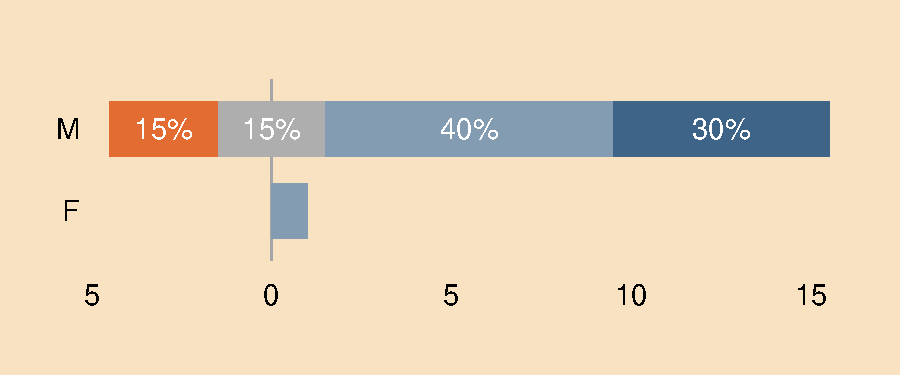
\includegraphics[align=t,trim={0mm 16mm 0 15mm},clip,width=8cm]{fig/workload/dirk_workload2aA.pdf}\\

    As above, for Researchers &
    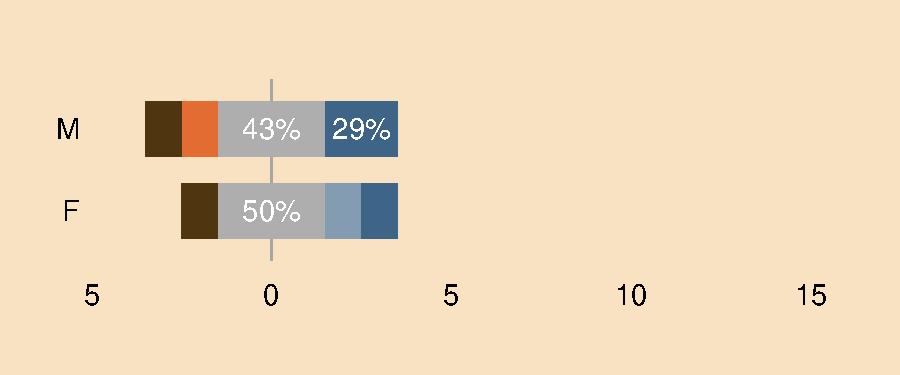
\includegraphics[align=t,trim={0mm 4mm 0 15mm},clip,width=8cm]{fig/workload/dirk_workload2aR.pdf}\\
    
    \hdashline
    
    Time spent completing my workload has changed (Academics) &
    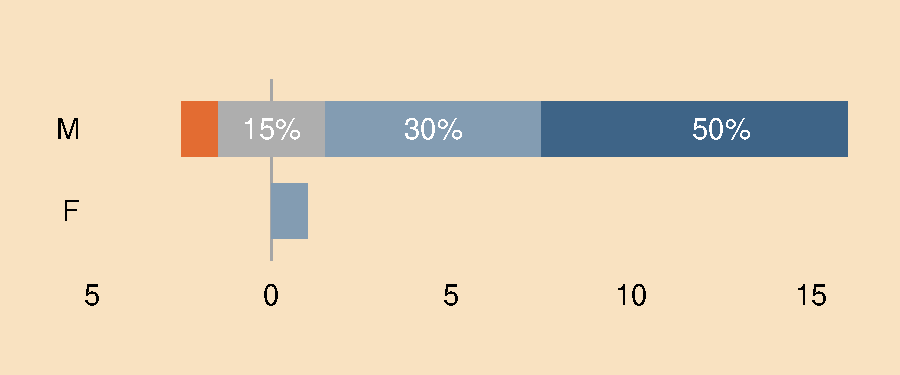
\includegraphics[align=t,trim={0mm 16mm 0 15mm},clip,width=8cm]{fig/workload/dirk_workload2bA.pdf}\\

    As above, for Researchers &
    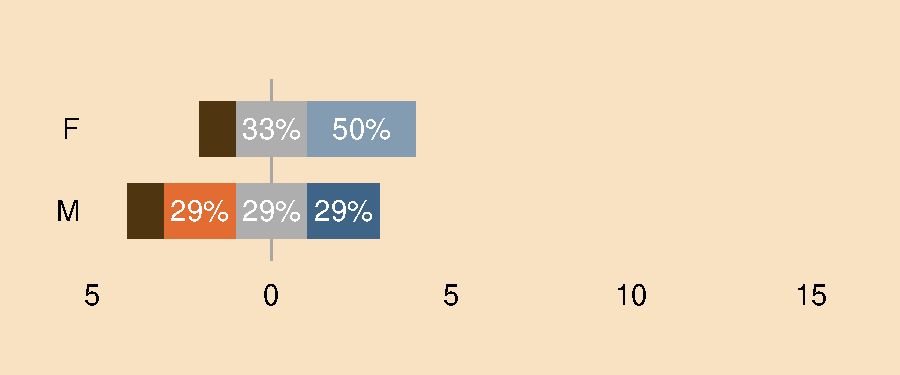
\includegraphics[align=t,trim={0mm 4mm 0 15mm},clip,width=8cm]{fig/workload/dirk_workload2bR.pdf}\\

    
    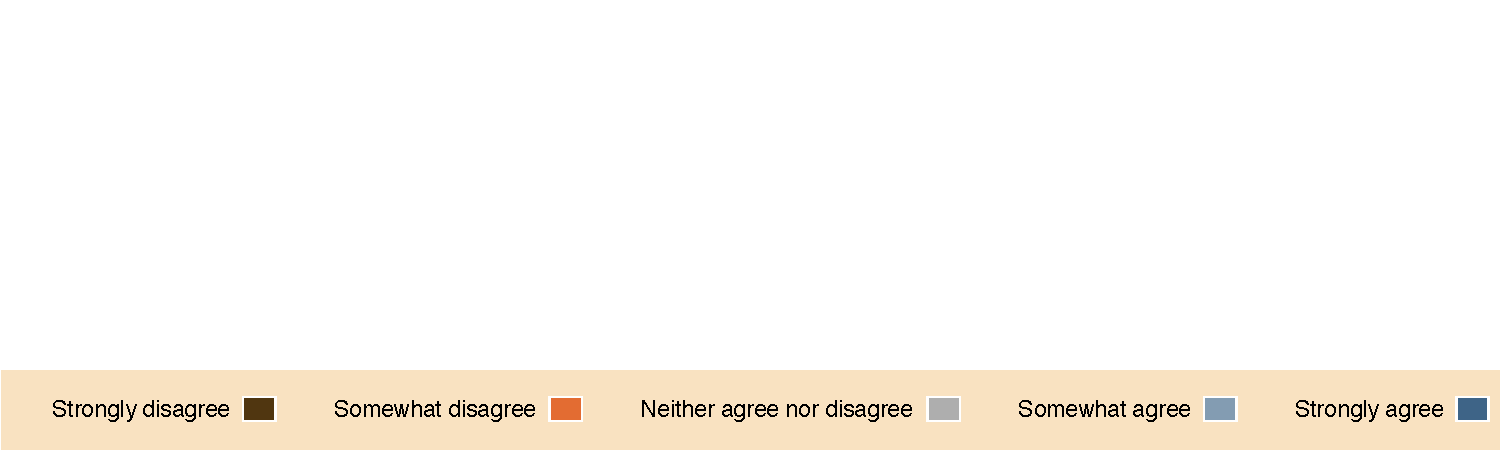
\includegraphics[trim={6mm 0 0 0},clip,width=14.5cm]{fig/legend5col.pdf}\\    
    \end{tabular}
\end{figbox}


The female academic felt that her workload was reasonable and balanced, that the scheme was transparent way, supporting her career goals. This did not change during the Covid-19 period (Figure~\ref{fig:workload} and Figure~\ref{fig:workloadchange}). 
Just over half of the male academics felt their workload allocation was reasonable and balanced; the majority felt that the allocation was clear and transparent. Only half said that the workload allocation aligned with their personal career development goals. Most male respondents felt that their workload was not balanced and had changed since the pandemic started. In the academic focus group, some colleagues commented on the ever-increasing number of administrative tasks, the scheduling of meetings, and the timing of tasks that may clash with caring responsibilities. 


\begin{myquote}
“Caring responsibilities are not considered when it comes to timing of meetings or academic responsibilities e.g. lecturing/labs. It is also not considered for workload.”
\end{myquote}

Both female and male  research staff respondents felt that their workload was reasonable and balanced (Figure~\ref{fig:workload}), whereas 50\% of female and male staff did not consider it to be clear and transparent. The majority of staff felt that their workload aligned with career development goals. However, problems remain:

\begin{myquote}
“If anything, the workload has increased considerably in the past 16 months [but] teamwork is good.”
\end{myquote}

In response, the school will review its workload model (Action~\ref{action:acad:transparentworkload}).


\begin{actionblock}{\ksspace{}Review workload model}{acad:transparentworkload}
\actreviewworkloadmodel
\hfill{
    \hypersetup{hidelinks}
    \hyperlink{c19}{\gotoactionsymbol{}}
}
\end{actionblock}




%% End of section.


\newpage

\newpage 
\section{Embedding policy, practice and supports to advance professional, managerial and support staff careers}
\label{sec:pms}

Professional, Managerial, and Support (PMS) staff as discussed in this section also includes research support staff, i.e. members of staff who perform primarily administrative tasks. 


\subsection{Reflecting on recruitment practices in the department, answer the following:}

\instr{
\begin{prompt}
\setlength\tabcolsep{6pt} 
\begin{tabu} to \textwidth { X[8] X X }    
     \multirow{2}{=}{Recruitment to PMS posts in the department adheres to institutional policy on recruitment, which includes gender-balanced panels and training for assessors.} & \textbf{Yes} & \textbf{No}  \\
     &  \XBox & \Square  \\ 
\end{tabu}
\setlength\tabcolsep{0pt} 
\end{prompt}

If you answered ‘no’, please comment.
}




\subsection{Provide three years of data on application, shortlist, and appointment rates for recruitment by gender and grade. Where data suggests opportunity for improvement, comment and reflect. Include any other relevant information relating to recruitment processes and practice for professional, managerial and support staff in the department.}



Gender specific data for selection committees and applications for the process of appointing PMS staff were not available at the time of application. However, partial records were gathered within CSIT (Tables~\ref{tab:selectioncommittee:pms}, \ref{tab:pms:appointment}). 

\input{tables2/tab_selection_pms}

\input{tables2/tab_appointment_pms}


Over a three-year period, there was a relatively even distribution of genders across those shortlisted.  
There is greater gender diversity among applicants for research PMS posts. However a challenge exists in attracting a gender-diverse pool of applicants to the school office (5 F) and systems administration posts (5 M). A male staff member was recruited to the school’s administrative group in 2018 but has recently moved to a research PMS role. 
Although 12 PMS staff took the EDI survey, only 1-3 responses were received for recruitment questions. Those that answered were content with the recruitment process.

The PMS working group discussed the causation, and mechanisms to address, gender imbalance. 
These included targeted recruitment strategies and making use of a gender language software to check for bias\footnote{\url{https://capd.mit.edu/resources/gender-decoder/}} in advertisements. The new \ac{EDI} implementation committee (EDIIC) will review the language used in advertisements to provide gender-neutral language (Action~\ref{action:acad:marketing},  Page~\pageref{action:acad:marketing}).

Furthermore, the PMS workgroup discussed how to convey the EDI-friendly ethos of the school. Action~\ref{action:pms:matchdescription} was proposed to review all school materials (images and text) to convey the flexible, inclusive and collegiate nature of the school. 

Periods of leave can have a negative impact on the career of women. The workgroup discussed how this situation may have worsened since the Covid-19 pandemic. As such, Action~\ref{action:acad:cvgaps} (Page~\pageref{action:acad:cvgaps}) was proposed to invite individuals to voluntarily account for documented leave, caring responsibilities, and pandemic-related gaps in their CV. 




The PMS workgroup discussions highlighted that the advertising template for research PMS positions is the same as that for academic researchers. The standard listed application criteria are not relevant to research PMS applicants, for example, a list of publications. This may deter suitably qualified potential applicants from applying for such research PMS positions. 
In order to prevent applicant confusion regarding what research PMS roles entail, potentially limiting the pool of applicants, Action~\ref{action:pms:matchdescription} is proposed. 



\begin{actionblock}{\ksspace{}Revise PMS application forms locally}{pms:matchdescription}
\actreviewadvertisements
\hfill{
    \hypersetup{hidelinks}
    \hyperlink{d3}{\gotoactionsymbol{}}
}
\end{actionblock}


Finally, part of Action~\ref{action:enrich:opportunities} (Page~\pageref{action:enrich:opportunities}) provides an opportunity for female undergraduate students to gain relevant work experience. This includes within the school's systems administration group, which could both provide an opportunity for female undergraduates students to gain experience and introduce some gender diversity to the systems administration team. 


\subsection{Reflecting on progression in your institution, answer the following:}
\instr{
\begin{prompt}
\setlength\tabcolsep{6pt}
\begin{tabu} to \textwidth { X[8] X X }
\multirow{2}{=}{Career progression opportunities for PMS staff are centrally managed by the institution (e.g. internal vacancy competitions; regrading; promotions pathway).} & \textbf{Yes} & \textbf{No}  \\
     & {\centering \XBox } & {\centering \Square}  \\ 
\end{tabu}
\setlength\tabcolsep{0pt}
\end{prompt}

If you answered ‘no’, please comment on the department’s role in career progression for professional, managerial and support staff. 
}

All administrative promotions are handled centrally by UCC.
The EDI survey and the PMS focus group indicated that most PMS staff have no interest in career progression. Some expressed a strong dissatisfaction with the lack of progression opportunities due to infrequent promotion calls and small quotas.  

\begin{myquote}
   ``I am not familiar with the promotion scheme. It does not apply to my case and therefore I have never expressed interest on it.'' 
\end{myquote}

\begin{myquote}
   ``I think it's quite clear that this is a problem across UCC. And the unfortunate thing is, it means that UCC doesn't get the best from staff.   People that are capable of doing more are not being given the opportunity to do that, and I think that's damaging to the whole institution.''
\end{myquote}



\subsubsection{Internal vacancy competitions}
Limited opportunities exist for progressing to senior grades via internal recruitment, usually requiring a move to a different unit.  This was perceived as uncertainty and risk, since PMS staff are largely happy working within the school: 



\begin{myquote}
    ``We want to progress but [also] to remain in the School ... because, well, I'm happy here.  And in order to [be] promoted, sometimes you need to go across campus and so that puts you off a bit because, you know, your well-being and being happy [are] very important.''
\end{myquote}

\begin{myquote}
     ``Moving from [one] department in the university to another department ... can cause issues.  It's almost treated like you're starting a new job [with a period of] probation ... If you're looking for loans, mortgages, things like that ... It seems like a kind of short-sighted thing to just default onto people.''
 \end{myquote}

\subsubsection{Promotion}
PMS staff expressed strong views on the lack of promotion opportunities, which had lain dormant for a long time. In recent years regular promotional calls (every three years) have become the norm for  PMS (and Academic) staff. The first of these calls was in 2019/2020, making 53 promotional posts available. No CSIT PMS staff member applied to this scheme. Another call has recently issued for 2022/2023. 

Some female PMS staff were sceptical of the process,  believing that interviewers lacked a first hand knowledge, or understanding, of the roles that applicants occupied at the time of application.


\subsubsection{Promotion pathways}

In the survey, PMSS were asked to reflect on the career progression opportunities (Figure~\ref{fig:survey:pms:careerprogression}). Apart from one male staff member, both genders agreed that promotions are free from gender bias. 
However, 2 females and 2 males were unsure how career breaks are considered in promotion decisions. The PMS Workgroup and focus group believed that the pandemic would likely have had a negative impact on promotion. This will be addressed with Action~\ref{action:acad:cvgaps} (Page~\pageref{action:acad:cvgaps}). 


PMSS did express a desire for greater training and guidance on preparing for promotion. Given the range of diverse PMS jobs available across the university, in schools and in central administrative units, one participant felt that guidance on potential PMS career pathways within the institution would be useful, to assist staff in identifying where and how their skills and experience might be usefully redeployed and expanded. Others concurred with this view.  

PMS staff training and career development will be discussed during PDRS meetings which will restart (Action~\ref{action:acad:pdrs}).





\begin{figbox}{!ht}
    \caption{Career progression process}
    \label{fig:survey:pms:careerprogression}
    

    \sffamily
    \footnotesize
    \raggedright

    \begin{tabular}{P{3.5cm}
                    !{\quad}
                    p{10cm}}
    \addlinespace
    The promotion criteria in UCC are transparent and fair.&
    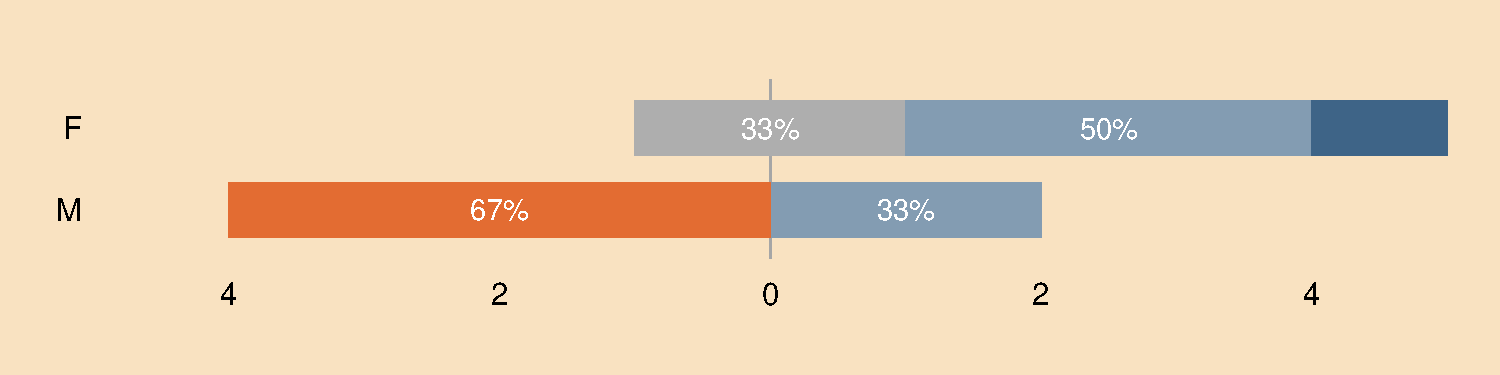
\includegraphics[align=t,trim={5mm 0 5mm 12mm},clip,width=10.5cm]{fig/pmscareer/fig231a.pdf}\\

\hdashline 

    The promotion process in UCC is transparent and fair.&
    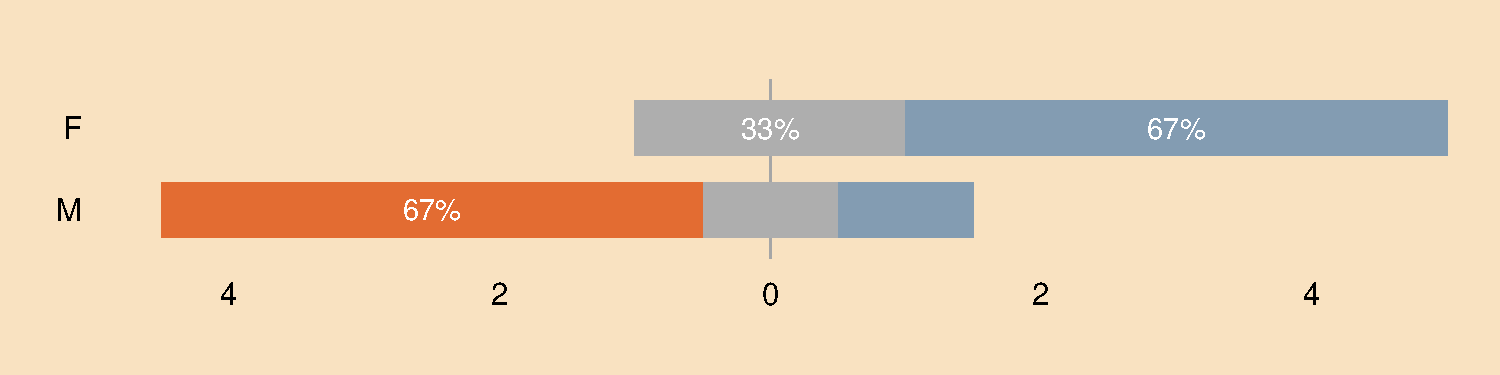
\includegraphics[align=t,trim={5mm 0 5mm 12mm},clip,width=10.5cm]{fig/pmscareer/fig231b.pdf}\\

\hdashline 

    Promotions are free of gender bias.&
    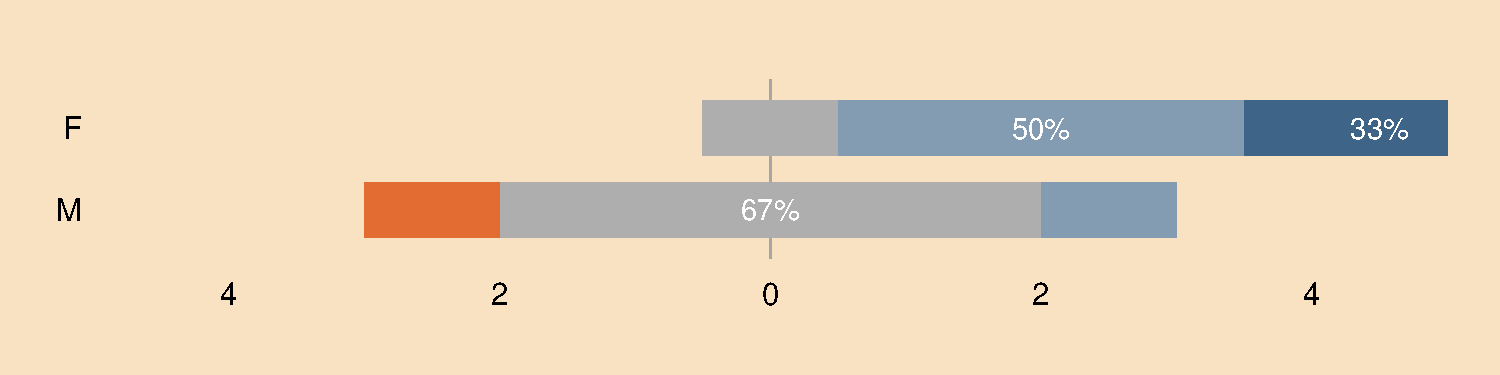
\includegraphics[align=t,trim={5mm 0 5mm 10mm},clip,width=10.5cm]{fig/pmscareer/fig231c.pdf}\\

\hdashline 

    It's clear how career breaks will be considered in promotion decisions. &
    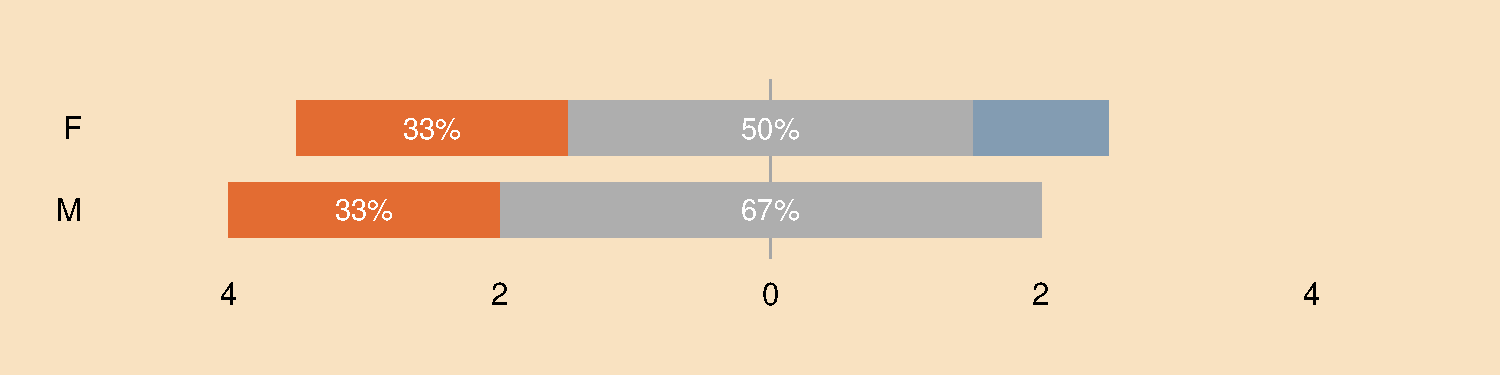
\includegraphics[align=t,trim={5mm 0 5mm 12mm},clip,width=10.5cm]{fig/pmscareer/fig231d.pdf}\\

\hdashline 

    Covid-19 has limited my promotion opportunities. &
    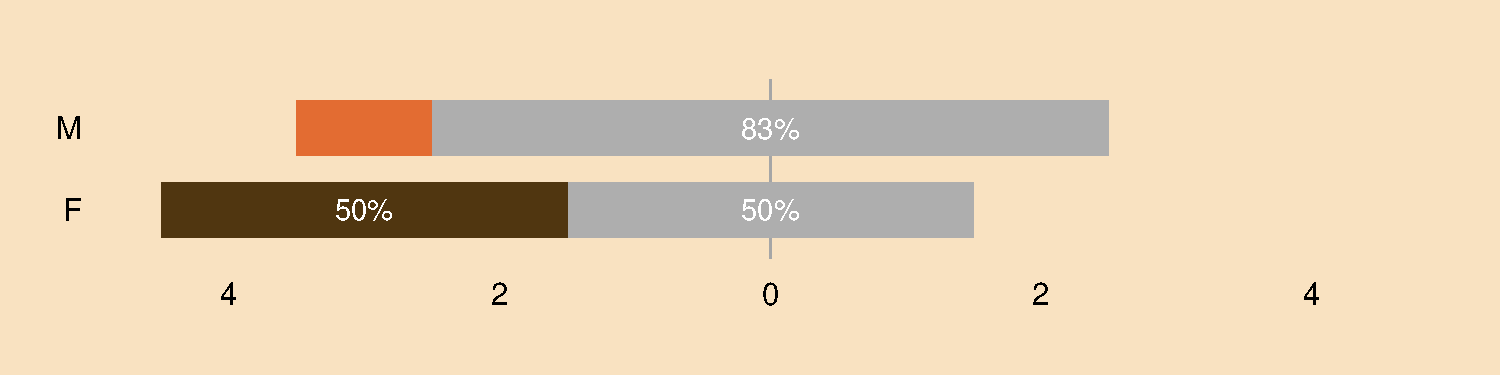
\includegraphics[align=t,trim={5mm 0 5mm 12mm},clip,width=10.5cm]{fig/pmscareer/fig231e.pdf}\\

    %% Legend
    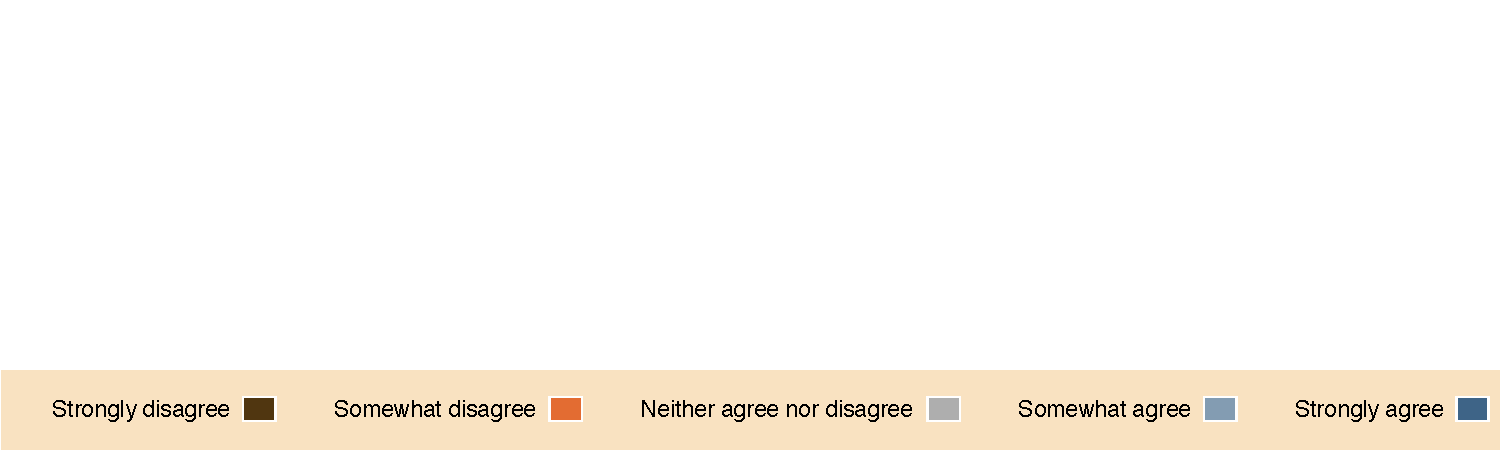
\includegraphics[trim={6mm 0 0mm 0mm},clip,width=14.5cm]{fig/legend5col.pdf}
    \end{tabular}
\end{figbox}




\newpage 
\subsection{Reflecting on opportunities for staff development review, answer the following:}

\instr{
\begin{prompt}
\setlength\tabcolsep{6pt} 
\begin{tabu} to \textwidth {@{} X[8] X X @{}}
     \multirow{2}{=}{The institution operates a development review process, or equivalent, for PMS staff} & \textbf{Yes} & \textbf{No}  \\
     &  \XBox & \Square  \\ 
\end{tabu}
\setlength\tabcolsep{0pt} 
\end{prompt}

If you answered `yes', comment and reflect on the implementation of this institution-level process in the department. This should include: 
\begin{itemize}
    \item data on uptake by gender;
    \item results from staff consultation presented by gender;
    \item information on any additional department-level opportunities for staff to discuss professional development, where different to above (2.\ref{sec:2e}). 
\end{itemize}
	
If you answered `no', provide detail on department-level opportunities for staff to discuss professional development, where different to above (2.e), including data on uptake by gender and results from staff consultation presented by gender. 
}


\subsubsection{Data uptake of development review process by gender}
As mentioned on Page~\pageref{acad:pdrs}, the \ac{PDRS} applies to all staff, and is due to resume in 2023 (Action~\ref{action:acad:pdrs}).
Table~\ref{tab:pdr:structure} indicates the line managers involved in the \ac{PDRS} for \ac{PMSS}.



\input{tables2/tab_pdr_structure}


\subsubsection{Results from staff consultation presented by gender}

The PMS staff were asked, in the staff survey,  to reflect on their opportunities to discuss career progress and promotion opportunities, Figure~\ref{fig:survey:pms:deptsupport}. 
Female staff were content with the opportunities available, there was some discontent amongst male PMS staff. Two male PMS staff members referred to a lack of opportunities within their roles to gain the experience required to meet promotion criteria. 

\begin{myquote}
    ``I think as well in the school there could be more done perhaps to allow staff to gain experience or to try different things, but in their roles.''
\end{myquote}


\begin{figbox}{!ht}
    \caption{Departmental support for career progression}
    \label{fig:survey:pms:deptsupport}
    

    \sffamily
    \footnotesize
    \raggedright

    \begin{tabular}{P{4cm}
                    !{\qquad}
                    p{10cm}}
    \addlinespace
    I am satisfied with the opportunities I have to discuss career progress with my line manager/HoD.&
    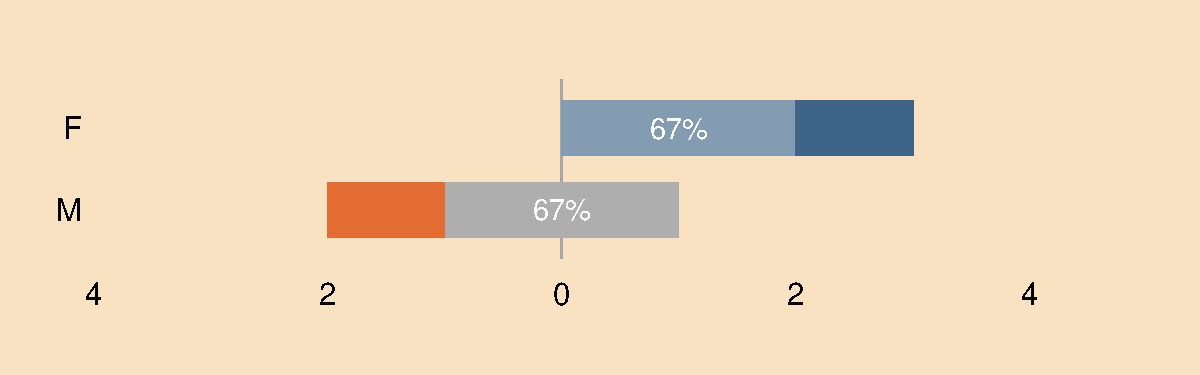
\includegraphics[align=t,trim={5mm 0 5mm 12mm},clip,width=9cm]{fig/pmscareer/ais_support1.pdf}\\

\hdashline 


    I am satisfied with the opportunities I have to discuss promotion opportunities with my line manager/Head of Dept.&
       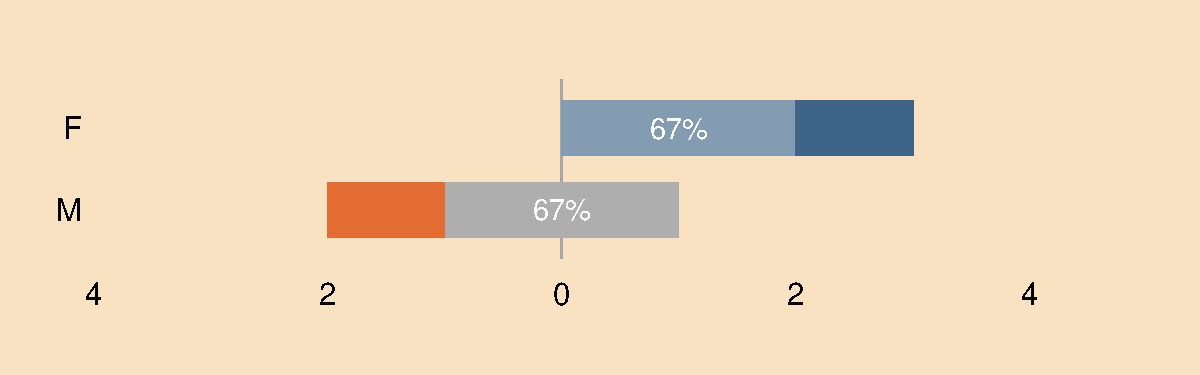
\includegraphics[align=t,trim={5mm 0 5mm 12mm},clip,width=9cm]{fig/pmscareer/ais_support2.pdf}\\

\hdashline

    I have opportunities in the School to get the experience I need in relevant activities to meet the criteria for promotion.&
       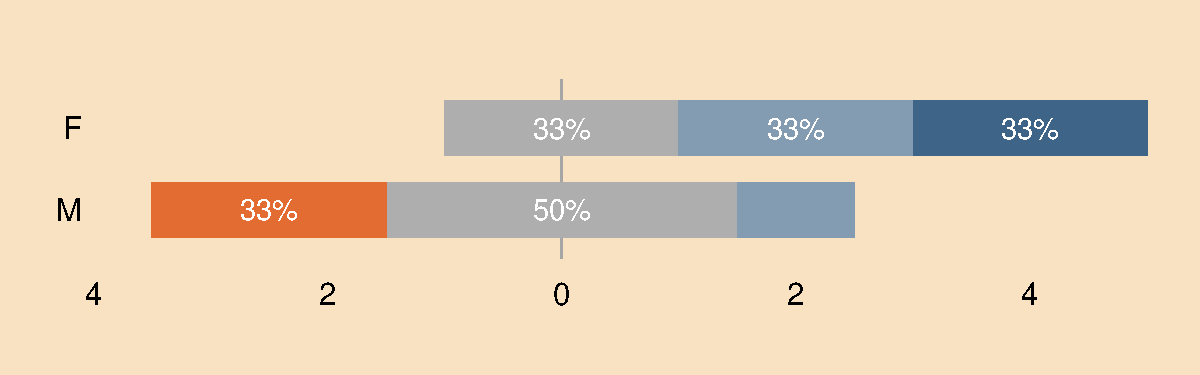
\includegraphics[align=t,trim={5mm 0 5mm 12mm},clip,width=9cm]{fig/pmscareer/ais_support3.pdf}\\

\hdashline 

    I have the support I need in the School to prepare and apply for promotion. &
       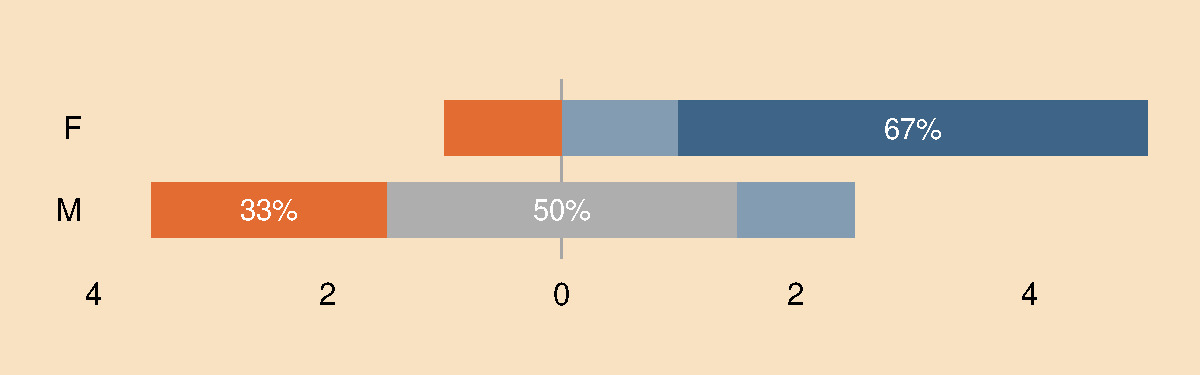
\includegraphics[align=t,trim={5mm 0 5mm 12mm},clip,width=9cm]{fig/pmscareer/ais_support4.pdf}\\


    %% Legend
    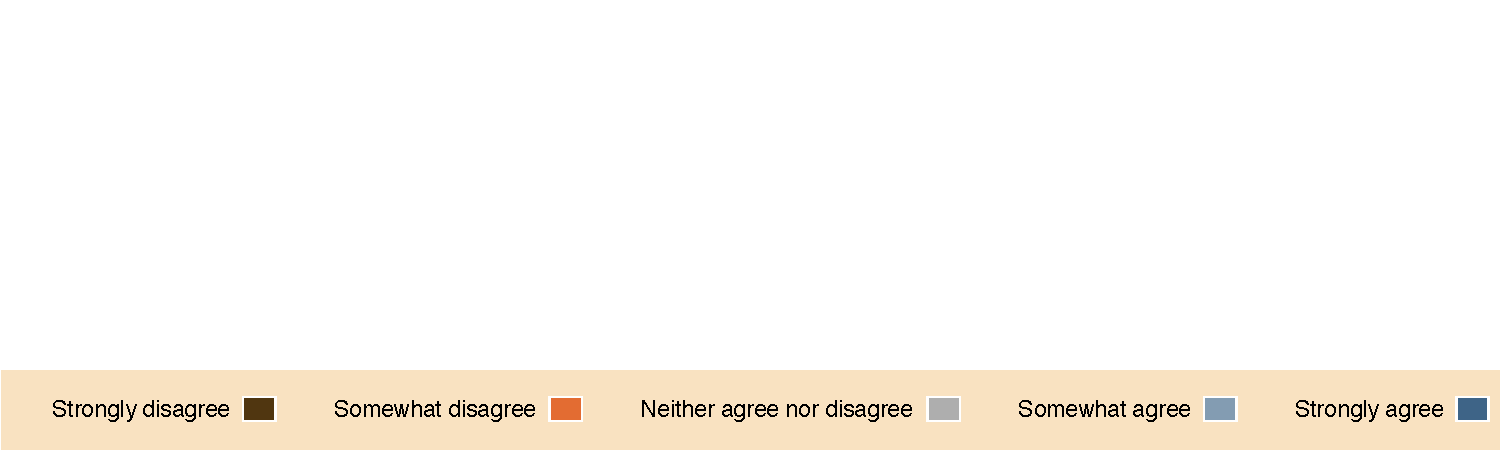
\includegraphics[trim={6mm 0 0 0},clip,width=14.5cm]{fig/legend5col.pdf}
    \end{tabular}

    
\end{figbox}

In the PMS focus group, despite the absence of formal reviews, participants reported strong satisfaction with the opportunities and support available to them to discuss their career/professional development with their line managers:
\begin{myquote}
    ``our line manager is very open to talking about career opportunities but obviously she has a limit. She can’t create promotion opportunities. She’s very supportive and does her best.''
\end{myquote}

\begin{myquote}
    ``There are opportunities to sit down with your line manager and get feedback. Because you know they’re very very open, the door is always open. But I suppose they’re also very restricted in what career path they can lay out for you and incentives to do well without promotional opportunities.''
\end{myquote}

To provide better support for PMS staff in their professional development,  Action~\ref{action:pms:experience} is proposed. 


\begin{actionblock}{\ksspace{}Opportunities for professional experience}{pms:experience}
\actpmsopportunities
\hfill{
    \hypersetup{hidelinks}
    \hyperlink{d8}{\gotoactionsymbol{}}
}
\end{actionblock}


\subsubsection{Information on any additional department-level opportunities for staff to discuss professional development, where different to above (2.e)}

PMS staff have expressed their desire for greater guidance and training for their professional and career development. 
We hope that the restarting of the PDRS (Action~\ref{action:acad:pdrs}) will help in this regard. 




\subsection{Comment and reflect on department engagement with institution-level supports for PMS staff career progression as well as any department-level support available, where different from above (2.\ref{sec:2f}). This should include results from staff consultation presented by gender.}

\input{tables2/tab_training_pms}

Although CSIT does not operate a formal policy of staff training for career development and progression, it raises awareness of training and progression opportunities. A wide range of training workshops are offered by the university, covering topics such as Teamwork, Leadership Potential, Leadership and Strategic Direction, People Management and Supervision, Management and Delivery of Results, and more.  Table~\ref{tab:training:pms} shows PMS staff engagement with these workshops in the 2017-2020 time period; on balance, there is an even uptake of opportunities among males and females. 




\input{2_3_fig233.tex}

PMS staff were asked in the staff survey to reflect on training supports for career progression with responses summarised in Figure~\ref{fig:survey:pms:trainingsupport}. 
Of the 12 PMS respondents, 6 answered this set of questions.  All female respondents were content with the training supports available. The male respondents expressed some minor discontentment. 



\subsection{Comment and reflect on how workload is distributed and managed. This should include information on how the breadth of professional, managerial and support roles and responsibilities are captured in workload planning and allocation and results from staff consultation presented by gender.}

\input{2_3_fig234.tex}

Non-research PMS staff workload is managed by the School Manager, subject to their specified responsibilities. The administrative support workload is distributed across
several categories, including academic support, outreach and student recruitment, finance, HR, and health and safety.
Workload is managed by the Computing Systems Manager based on function and matched to the expertise of the staff member.
Functions include IT support, core systems/services, and teaching support.



The workload of the research PMS staff is managed by the general manager of one of the research centres (Table~\ref{tab:researchcentres}), or by a specific \ac{PI} in the case of smaller research units. 



PMS staff were asked to reflect on their workload allocation (Figure~\ref{fig:survey:pms:worklife}), if it was transparently allocated and if it aligned with their career goals.
Generally, the female staff had no opinion or were happy (one was not). The male staff members were marginally less satisfied. 






The pandemic had some influence on people's workload, as reflected in the comments: 
\begin{myquote}
``my workload seems to have increased as many more formal meetings.''
\end{myquote}
\begin{myquote}
``If anything, the workload has increased considerably in the past 16 months.''
\end{myquote}
\begin{myquote}
``Work is more intense since March 12 2020 [the date of the first Covid-19 lockdown]''
\end{myquote}






\newpage

\clearpage

\section{Evaluating culture, inclusion and belonging}
\label{sec:culture}

\subsection{Provide information on how the department ensures that culture and practices support inclusion and belonging. This should include, but is not limited to, information on how the department actively considers gender equality, and EDI more broadly, in:} 
\instr{
\begin{itemize}
\item	organisation of meeting and events;
\item	images and text used in department spaces and on the department’s website; 
\item	student curricula, pedagogy, and assessment. 
\end{itemize}
}


\subsubsection{Organisation of meetings and events}\label{sec:events}
CSIT organises a variety of school meetings, committees, social events and research seminars.  
Social events are normally organised for staff at Christmas and in summer. The school aims to promote inclusion by organising social events around staff availability. 

%\begin{figbox}{!b}
\begin{figure}[!b]
\caption[Meetings and social events]{Meetings and social events. Left: Prof John Morrison, Chair of the SAT, presenting an update at a hybrid school meeting. Right: social event at Christmas 2017}
\label{fig:schoolmeeting}
\begin{tabular}{c !{\quad} c}

    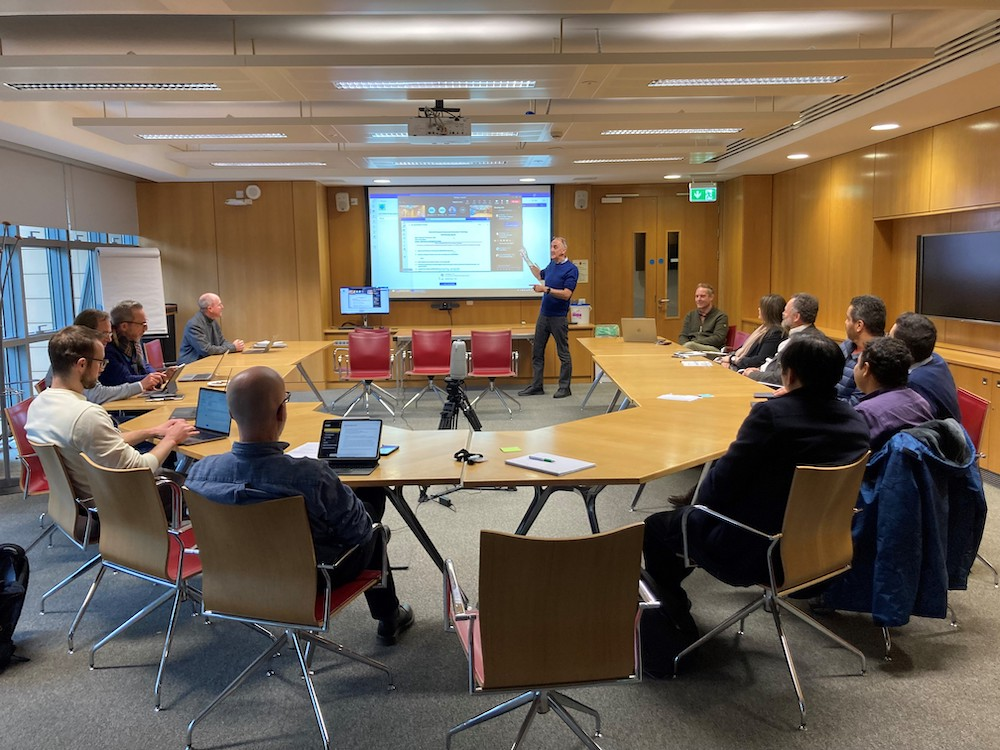
\includegraphics[width=2.85in]{img/JM at school meeting.jpg}    &
    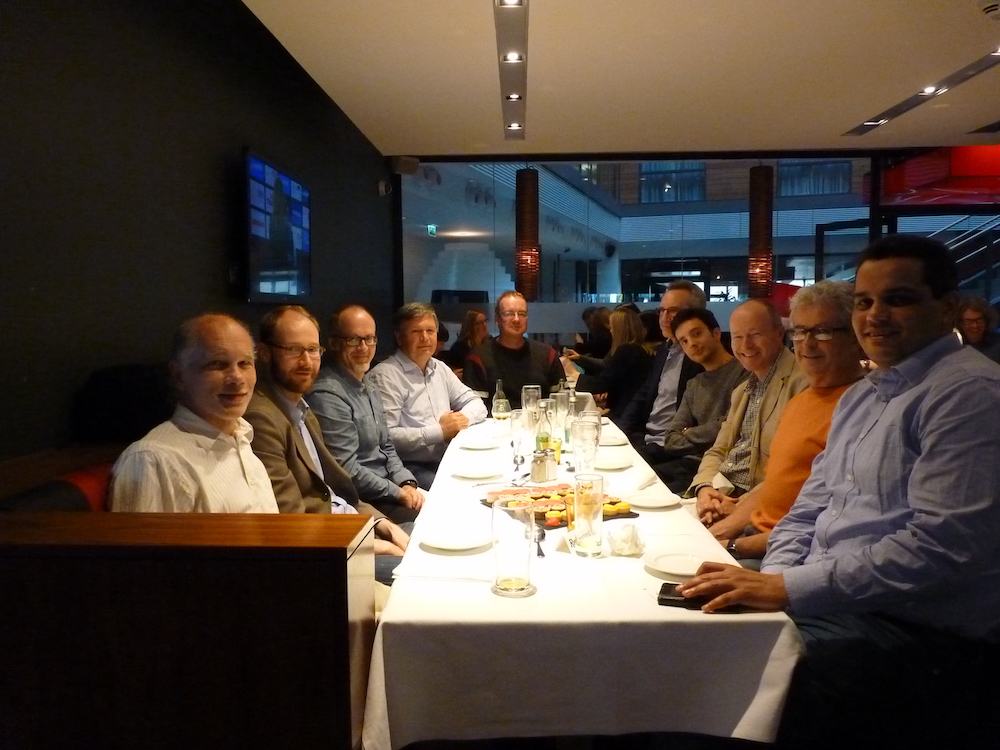
\includegraphics[width=2.85in]{img/XMas2017.JPG}\\
    \end{tabular}
\end{figure}
%\end{figbox}

School meetings are scheduled for the last Friday of each month at 15:00, and finish by 16:30. These meetings are chaired by a senior member of staff, and all staff are invited to submit agenda items in advance. 
During the meetings, staff are encouraged to speak freely.

The school organises regular seminars with internal and external speakers. Survey data show that many staff (68\% female, 58\% male) value gender-balance in seminars, workshops and symposia. However,  42\% of females and 32\% of males do not feel men and women are evenly represented among speakers and chairs. Since 2022, staff proposing a male speaker are also strongly encouraged to suggest a female speaker in addition. This has resulted in a better gender balance among speakers (Table~\ref{tab:seminars}).




\input{tables2/tab_seminars}

The survey data indicate research staff and PhD students perceived a lack of events and opportunities where they could engage with the school staff. 
Most networking, job opportunity and professional development events are organised by the research centres (Section~\ref{sec:overview}). Although open to all, centres tend to announce these events only to their members, leaving many unaware of these opportunities. Consequently, not all have the same experience and may feel disconnected from the greater school.
This disconnection is accentuated by having PhD students located in centre-specific, access-controlled, laboratories, thus limiting interactions among students working in different areas. 

CSIT does not offer formal researcher orientation. Newcomers are not explicitly made aware of the structure of the school, the research centers, and any opportunities that may exist for teaching and laboratory assistance, leading to Action~\ref{action:acad:handbook}.
These issues make it difficult to promote a culture of inclusivity within the school, and may adversely affect the quality of the research by not promoting a culture of multi-disciplinary collaboration (Action~\ref{action:cult:researchinteraction}).


\begin{actionblock}{\ksspace{}Increase opportunities for researchers to interact}{cult:researchinteraction} 
%\todo{Should this be more like: increase opportunities for researchers to interact?}
\actimproveinteraction
\hfill{
    \hypersetup{hidelinks}
    \hyperlink{e2}{\gotoactionsymbol{}}
}
\end{actionblock}


\subsubsection{Images and text used in department spaces and on the department's website}
The school's website (\url{https://www.ucc.ie/en/compsci/}) is used to promote its academic programmes and research activities. Graduations, undergraduate events and outreach events are detailed in the news section.  

Students from all programmes are invited to share their experiences. Currently, the site includes six testimonials (4F, 1M) of our students.

\begin{figbox}{!ht}
    \caption{Testimonials on the CSIT website}
    
\includegraphics[width=14.2cm]{img/csitwebsite.jpg}  
    
    \begin{tabular}{c
                    !{\quad}
                    c}
         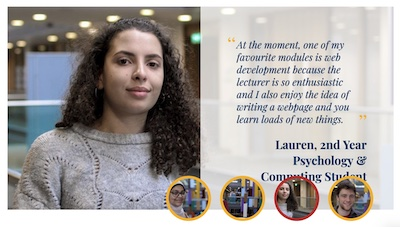
\includegraphics[align=t,height=3.8cm]{img/testimonial-lauren.JPG} 
         & 
         
\includegraphics[align=t,height=3.8cm]{img/testimonial-yomna.JPG} \\
         
    \end{tabular}
\end{figbox}

\subsubsection{Student curricula, pedagogy, and assessment}
The school offers a range of degree programmes (Table~\ref{tab:programmeoptions}), and has two committees concerned with curricula, pedagogy, and assessment: the \ac{APCD} reviews proposals for new academic programmes and changes proposed to programmes and modules; the \ac{TLSE} is concerned with the teaching and learning experience. 

\input{tables2/tab_programme_options}


Before the \ac{AS} process, no systematic consideration was given to how equality and diversity issues might be used to enhance the curriculum. A first step will be to use school-specific data from the university’s biannual EDI Student Survey to uncover the specific needs of students with diverse backgrounds.  

The TLSE Committee will use tools developed through the DISCs project (Disciplines Inquiring into Societal Challenges),  a collaborative study between UCC, \ac{DCU} and \ac{MU} to develop tools to support the professional development of teaching staff in HE in themes of gender consciousness, interculturalism and community.

We will also participate in UCC EDI-organised briefing sessions on EDI in Teaching \& Learning, planned for 2023/24 (Action~\ref{action:cult:backgrounds}).


\begin{actionblock}{\ksspace{}Guidelines for addressing needs of students from diverse backgrounds}{cult:backgrounds}
\actcultbackground
\hfill{
    \hypersetup{hidelinks}
    \hyperlink{d10}{\gotoactionsymbol{}}
}
\end{actionblock}




\subsection{Comment and reflect on the department’s current understanding of, and capacity to identify and address, issues and opportunities relating to equality grounds in addition to gender, as well as capacity to identify and address intersectional inequalities for staff and students.}

School staff and students come from varied ethnic backgrounds and we are just embarking on our journey to build capacity to understand and address inequalities affecting underrepresented groups, and intersectional inequalities. The self-assessment process has revealed a need to build a better awareness of how intersecting identities contribute to experiences of discrimination and disadvantage. We are beginning this work with encouraging all staff to participate in the IHREC\footnote{Irish Human Rights and Equality Commission, \url{https://www.ihrec.ie/}} eLearning module on ‘Equality and Human Rights in the Public Service’ and UCC’s EDI in \ac{HE} programme (including a module on race awareness and anti-racism in HE) (Action~\ref{action:cult:backgrounds}). 



Of particular importance to the school are two socio-economic factors that, combined with gender, can significantly disadvantage staff and students. The first is income and job insecurity for fixed-term staff. The second is lack of affordable accommodation. The ongoing housing crisis across Ireland, including in Cork, affects staff and students who are renting. Junior academic and research staff, in particular, struggle to secure accommodation. New international staff and students are disproportionally affected. The school has identified the accommodation crisis as a key issue for recruitment and retention of staff at all levels. The \ac{HOS} is actively advocating at university level for the implementation of measures  to mitigate the impact of this crisis.



\subsection{Provide information on the department’s culture as it relates to gender equality and, where relevant, EDI more broadly, by presenting consultation findings by gender and staff category on the following areas:}
\instr{
\begin{itemize}
\item	values and traditions of the department;
\item	formal and informal structures and interactions that characterise the working and learning environment of the department, including leadership practices and behaviours;
\item	negative practices and behaviours and how these are managed by the department; 
\item	flexible working opportunities in the department;
\item	management of, and attitudes towards, family leave in the department. 
\end{itemize}
\vspace{2mm}
\noindent Where data suggests opportunity for improvement, comment and reflect. This should include reflection on any gaps between institution-level policy and practice in the department, including if the institution’s approach meets the requirements of department staff.
}

\subsubsection{Values and traditions of the department}
There is strong collegiality within the school. The survey data (Figure~\ref{fig:treated2}) show most staff feel they belong and included. There are clear values and expectations on how people should behave towards each other. Staff also believe they are treated fairly, without regard to gender, civil or family status, sexual orientation, religion, age, disability, race or membership of the Traveller community.


\input{2_4_survey_positive.tex}

All staff  are invited to school social activities. The school supports various social events for students and staff. For example, several online quiz nights were organised for postgraduate students during the pandemic. The school organises an annual reception for international students attended by the \ac{HOS}, Programme Directors, and staff from the university's \ac{IO}. 
Other social events include weekly social meetings for researchers, and a well-attended PhD climbing wall event (Figure~\ref{fig:socialevents}). 

\begin{figure}[!ht]
\caption{Social events with students and members of CSIT}
\label{fig:socialevents}
\begin{tabular}{l
                !{\quad}
                r}
     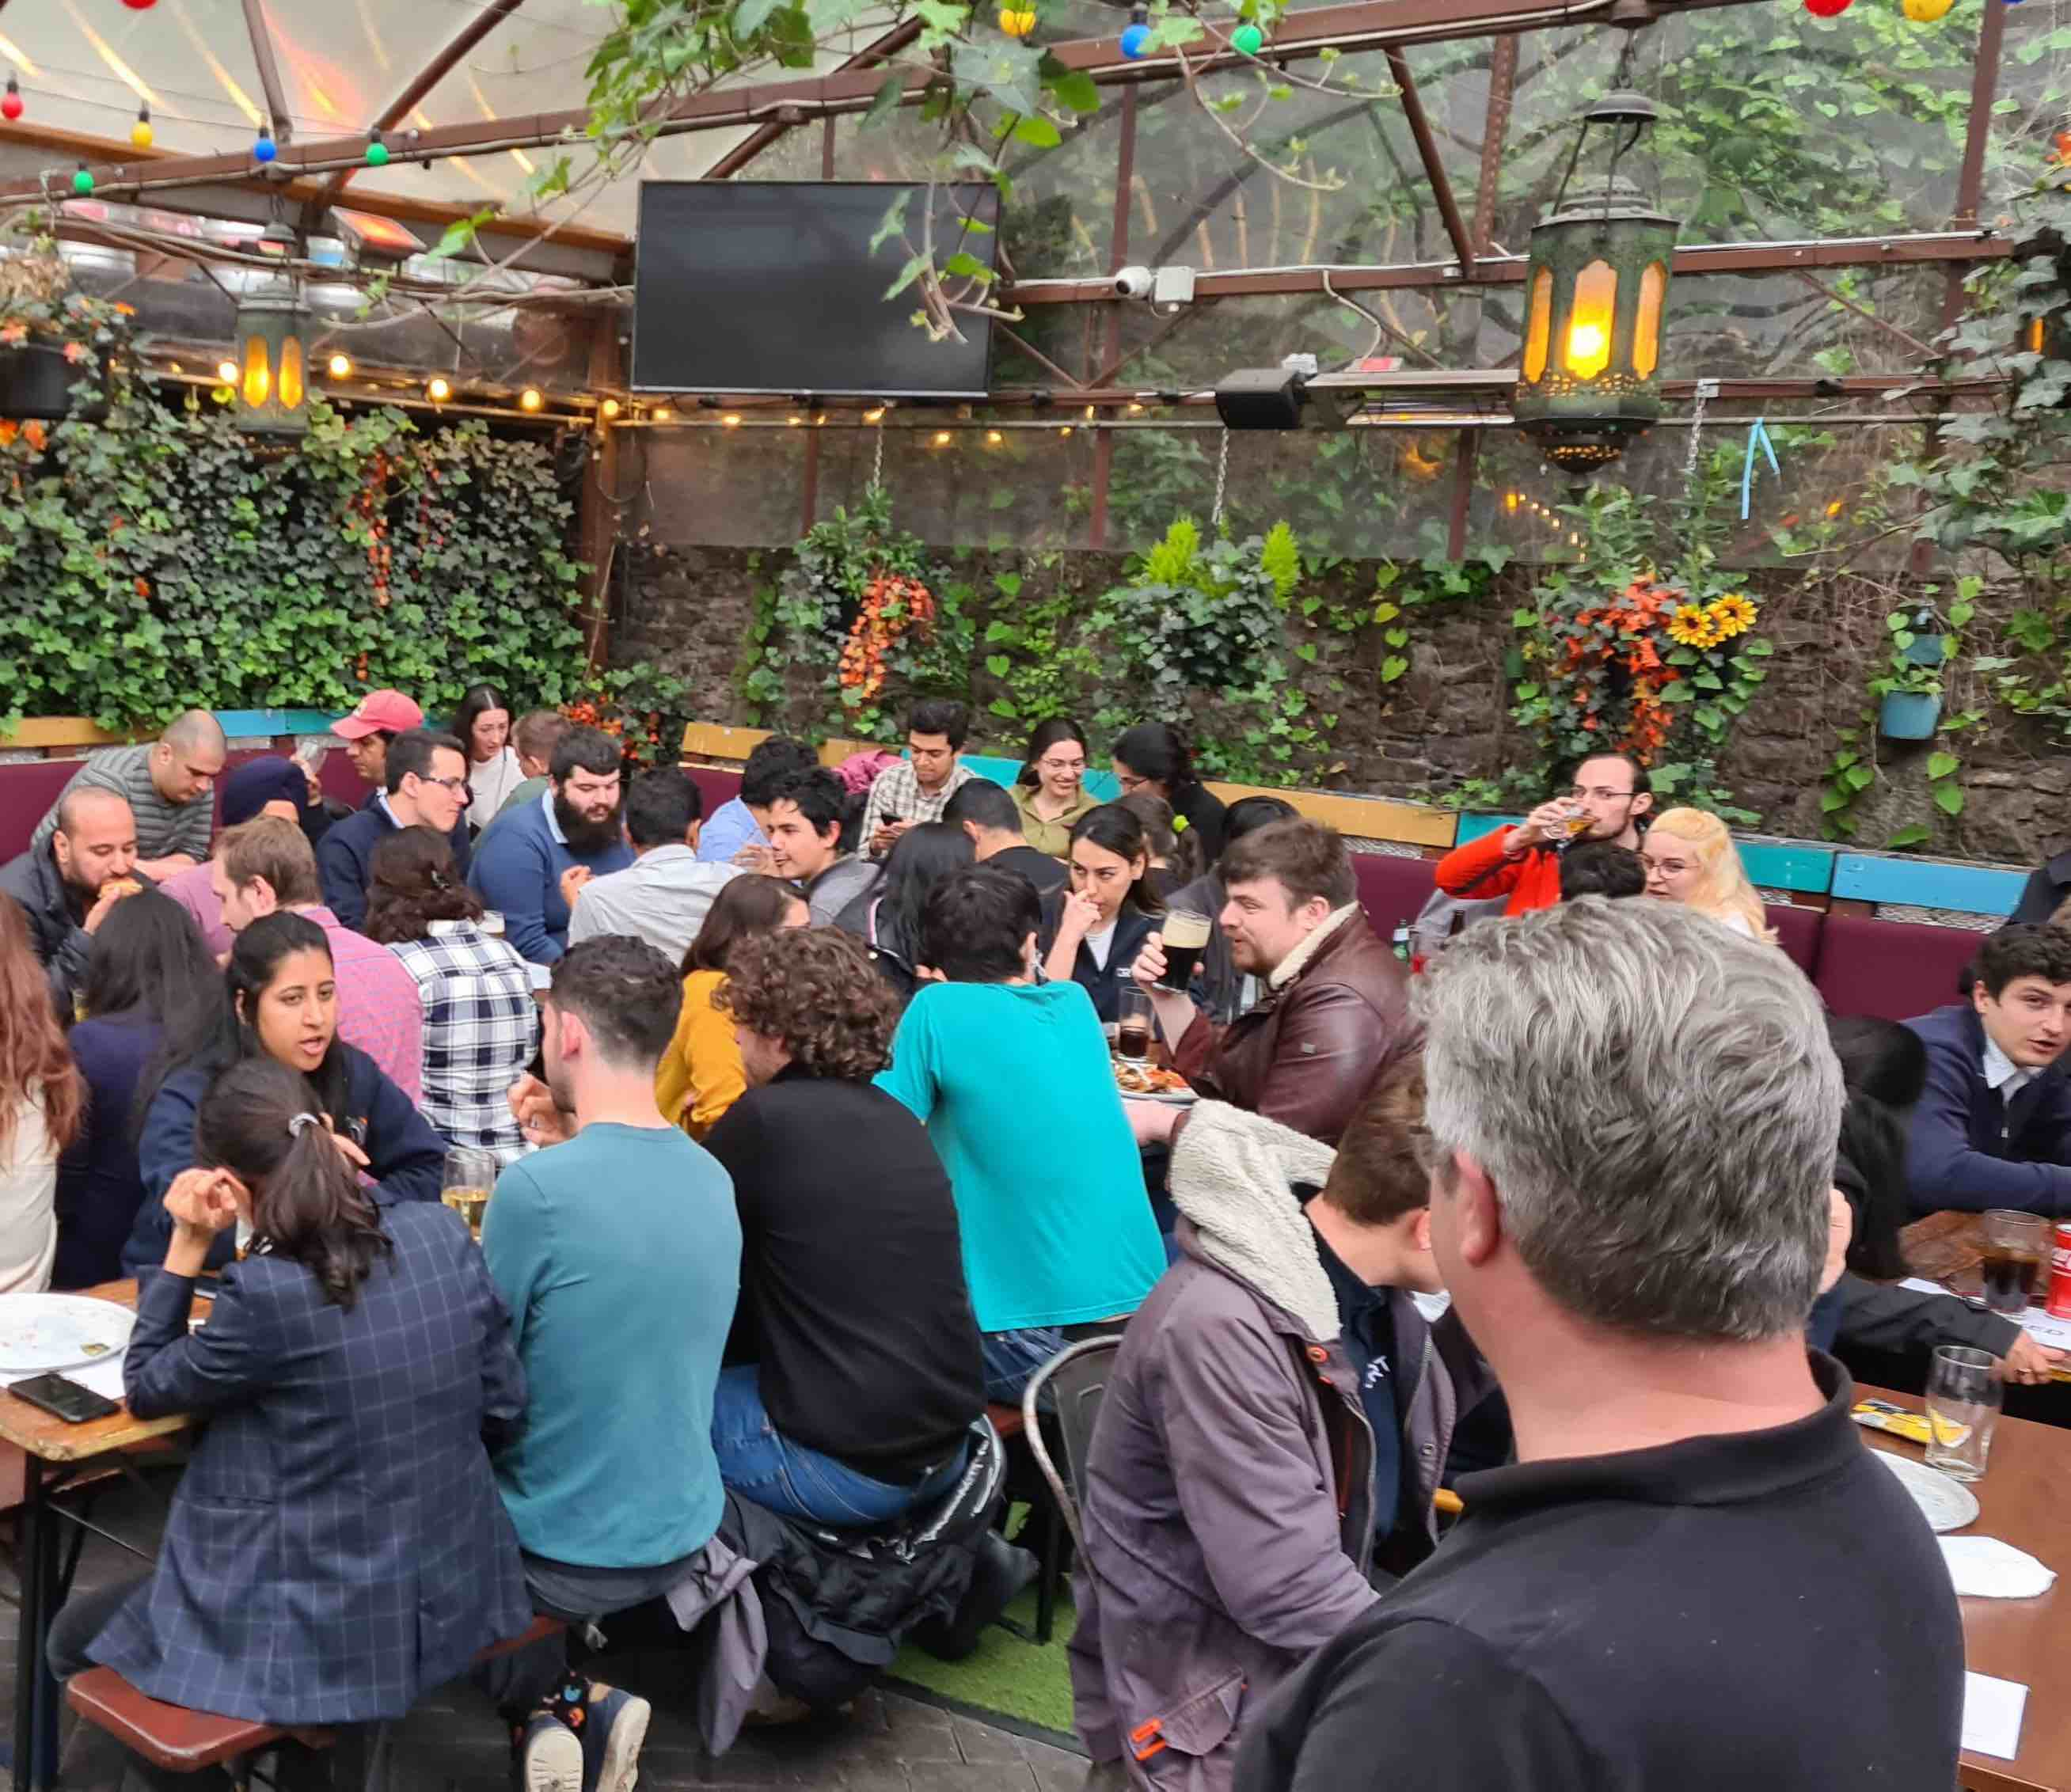
\includegraphics[height=5.8cm]{img/socialouting1.jpg} 
     & 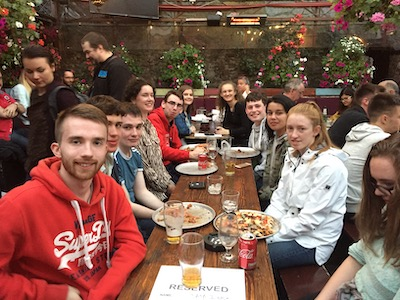
\includegraphics[height=5.8cm]{img/socialouting2.jpg}  \\  
     \addlinespace
     \multicolumn{2}{c}{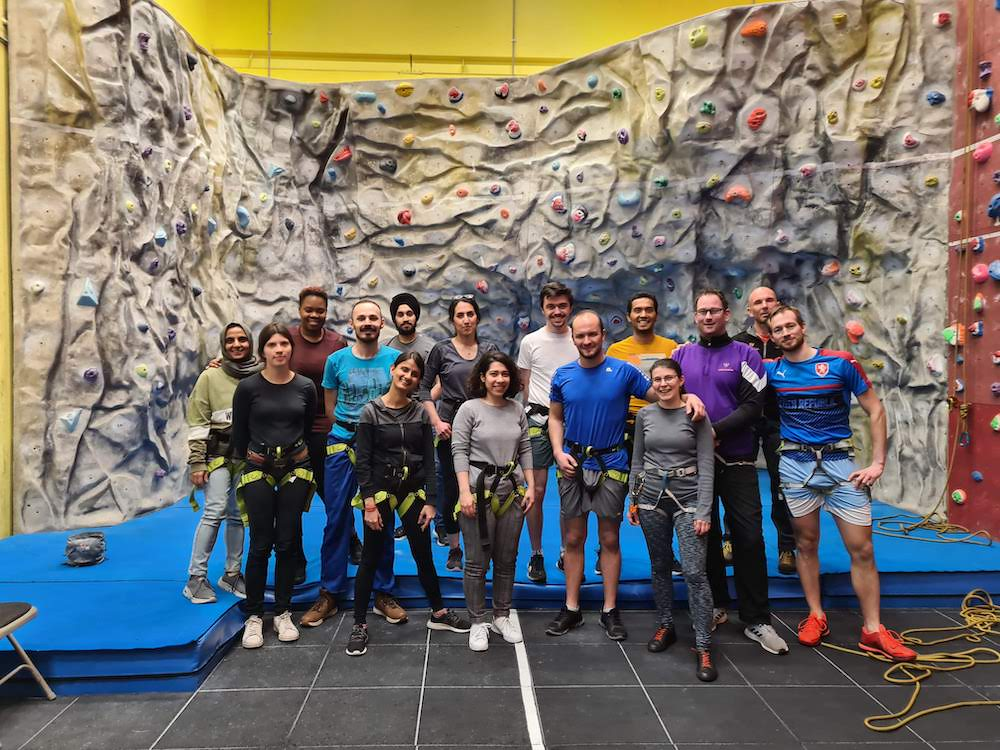
\includegraphics[trim={0 4cm 0 4cm},clip,width=15cm]{img/wallclimbing.jpg}}\\
\end{tabular}
\end{figure}




\subsubsection{Formal and informal structures and interactions characterising the department's working and learning environment, including leadership practices and behaviours}

New staff are assigned a mentor for orientation and to provide guidance on academic career development.

The school supports staff and students in grant and scholarship application (Section~\ref{sec:academic}) and communicates and encourages female-targeted students' scholarships (e.g., Google stipend)  (Section~\ref{sec:overview}). 

The \ac{HOS} recently introduced strategies to support minorities in our international student cohort.  For example, establishing an international student mentor role to advise international students on  academic and non-academic matters. 

In 2023, the school accepted 3 Ukranian student refugees. 



\subsubsection{Negative practices and behaviours and their management by the department}

No specific negative behaviour by staff or students was reported in either the survey or focus groups. Nevertheless, it is school policy to  act in accordance with university policy to address any such behaviour, should it arise. 

Survey data (Figure~\ref{fig:treated1}) indicate that if witnessing others being unfairly treated, they would mostly feel comfortable reporting it.
While the vast majority of staff can identify a safe person to report unfair treatment in the school, a minority of staff feel reporting unfair treatment could affect their career. The reasons behind these answers will be explored in the progress review undertaken by the EDIIC in Year 3 (Action~\ref{action:intro:review:year3}). 


\input{2_4_survey_negative.tex}





\subsubsection{Flexible working opportunities in the department}

The school currently supports flexible working for all staff.  Most staff are facilitated to work from home under the Pilot Blended Working Policy, subject to the nature of their job.
The PMS staff focus group and the staff survey indicated strong support for blended working to continue. Staff want the university to provide a clear and transparent policy (Action~\ref{action:cult:flexwork}) and that every effort should be made to maximise flexibility at school level. 

\begin{actionblock}{\ksspace{}Flexible working}{cult:flexwork}
\actadoptflex
\hfill{
    \hypersetup{hidelinks}
    \hyperlink{e5}{\gotoactionsymbol{}}
}
\end{actionblock}
 
The school's reception is open daily from 9:00 to 17:00. This limits some PMS staff from availing of flexible start and finish times. Many working arrangements are agreed with line managers subject to university policy. Some academics may indicate preferences for certain time slots for laboratory sessions, though room and student availability must be considered. 

Staff in focus groups reported they felt comfortable discussing flexible working arrangements with their line manager. Survey data show most staff are confident of a positive outcome (86\% females and 85.7\% male agree/strongly agree). Researchers, in particular, feel comfortable discussing work life balance issues with their PI (86\% females and 100\% male agree/strongly agree). 



\subsubsection{Management of, and attitudes towards,  family leave in the department}

Table~\ref{tab:culture:leave} reports various types of family-related leave during 2017-2020 by CSIT staff.
Family leave policies are determined by the university but the school is responsible for arranging cover. 
It was noted that UCC currently requires staff to have a minimum of six months service to qualify for paid maternity leave. Action~\hyperlink{act556}{5.5.6} in the \textit{UCC Institutional Bronze Application 2019} addresses this issue:  

\begin{UCCaction}{5.5.6}{}\hypertarget{act556}
Review  the  gender  impact  of  the  requirement  for  26  weeks  continuous  service  in order to be eligible for paid UCC maternity leave.
\end{UCCaction}

\input{tables2/tab_leave}

The academic focus group reported  a supportive environment for colleagues taking maternity and paternity leave; two colleagues returning from maternity leave and long-term medical leave were offered a reduction in teaching for the first semester on return.  
Participants commended both the current and previous Heads of School for their support for leave-takers. 
No formal backfill policies exist at the university level for leave other then for maternity and sick leave.

\begin{myquote}
    ``so it's up to the Head of School to try and find a way to cover your classes [and] reduce [your] teaching load for that semester.''
\end{myquote}

In the absence of an institutional commitment, Heads of School carry a responsibility that some focus group participants felt to be unreasonable.  This ad-hoc arrangement means that  leave-takers are dependent on the goodwill of the \ac{HOS} and puts increased demand on the goodwill of colleagues to cover during a period of leave.  
Leave-takers can feel a sense of responsibility and guilt for burdening colleagues with increased workload; this in turn might deter people from taking statutory leave:    

\begin{myquote}
“You feel bad about [taking leave] because you're basically asking [colleagues] to [cover your] classes ... It's very awkward, and that has nothing to do with the willingness of the Head of School. As I said, [they’re] very supportive, but it's all managed informally. They have to try and help you without getting any [support themselves], pretty much.”  
\end{myquote}

The policy for research students states that a pregnant student should notify her supervisor and independently identify options open to her from her funder
(Action~\ref{action:cult:famleave}).


\begin{actionblock}{\ksspace{}Supporting family Leave}{cult:famleave}
\actremoveimpediments
\hfill{
    \hypersetup{hidelinks}
    \hyperlink{e5}{\gotoactionsymbol{}}
}
\end{actionblock}





\newpage
\section{Department priorities for future action}
\label{sec:priorities}

\subsection{Identify the department’s key issues relating to gender equality and establish key priorities for action over the next four years:} \instr{
\begin{itemize}
    \item Select up to five key priority areas where the department will strive for impact. Selected priorities should be justifiable and based on the quantitative and qualitative evidence presented in Section 2.
\item	Specific action(s) to support progress in priority areas should be identified. 
\end{itemize}
}





\subsubsection{Select up to five key priority areas where the department will strive for impact.
Selected priorities should be justifiable and based on the quantitative and qualitative
evidence presented in Section 2. Specific action(s) to support progress in priority areas should be identified.}




%\begin{itemize}[label=\textbf{\arabic*}]

\paragraph{Challenge}
The school has no formal structures nor has had discussions relating to a culture of gender equality and diversity. 

\begin{priority}{1}
 Develop the governance, structures, policies and procedures to deliver the AS action plan and imbed the AS Ireland Principles in the school.
\hfill{
    \hypersetup{hidelinks}
    \hyperlink{p1}{\gotoactionsymbol{}}
}
\end{priority}


A first action is to establish a gender balanced EDI Implementation Committee (EDIIC), and appoint a Chair from amongst the senior staff (Action~\ref{action:intro:edi}). The committee will have the authority to oversee the implementation of the action plan and develop a positive EDI culture in the school. 


\paragraph{Challenge}
Computer Science is a male-dominated discipline; Priorities \hyperlink{priority:2}{2}  and \hyperlink{priority:3}{3} will address the gender imbalance in CSIT staff (23\% F) and student (26\% F) cohorts.

\begin{priority}{2}
    Increase the ratio of female applicants for staff posts (Academic / Research) to improve gender balance.  
    \hfill{
    \hypersetup{hidelinks}
    \hyperlink{p2}{\gotoactionsymbol{}}
}
\end{priority}


%The main actions include improving the advertising materials to appeal to female applicants and to use female targeted initiatives.   

\begin{priority}{3}
    Increase the number of female students registered in UG and PG programmes. 
    \hfill{
    \hypersetup{hidelinks}
    \hyperlink{p3}{\gotoactionsymbol{}}
}
\end{priority}

Gender imbalance is more pronounced at undergraduate level, particularly in our flagship BScCS programme (14\%). The school will survey our UG students to understand what motivated them to study Computer Science (Action~\ref{action:survey:females}). It will enrich opportunities for female students to gain work experience, for example, through internships in the school (Action~\ref{action:enrich:opportunities}). Boosting the visibility of successful female researchers, alumni, and professionals will provide role models for new recruits and current students (Action~\ref{action:boost:visibility}).  

The actions associated with this priority area will provide information to improve our future recruitment strategies, deepening the pipeline for research and academic careers in Computer Science. 

\paragraph{Challenge}
Due to the lack of formal Professional Development Reviews (PDR) and mentoring in recent years, more support is required for staff career development and progression. 
There is a dearth of female academic (9\%) and research (17\%) staff in the school, with none at senior grades.  The school had no permanent female academic staff member until 2017.


\begin{priority}{4}
Supporting staff development to further career progression.
\hfill{
    \hypersetup{hidelinks}
    \hyperlink{p4}{\gotoactionsymbol{}}
}
\end{priority}


  
The key actions to deliver on this priority include restarting the Performance Development Review System to support staff career development (Actions~\ref{action:acad:pdrs}, \ref{action:acad:mentorresearchers}). Improved mentoring for interested staff, career training and research funding workshops will be conducted (Actions~\ref{action:acad:mentoring}, \ref{action:acad:supportfunding}).  

\paragraph{Challenge}
Staff would like to see more family-friendly policies, more diversity and inclusivity in staff and student cohorts.

\begin{priority}{5}
Promote a culture of inclusivity and belonging.
\hfill{
    \hypersetup{hidelinks}
    \hyperlink{p5}{\gotoactionsymbol{}}
}
\end{priority}

The key actions under this priority are both inward and outward focused.  The inward actions include supporting family / flexible leave and more integration of all research groups in school events (Actions~\ref{action:cult:famleave}, \ref{action:cult:researchinteraction}).  The outward facing actions concentrate on ensuring that schools from diverse backgrounds are a focus of attention (Action~\ref{action:cult:backgrounds}).




\subsection{Outline how the department’s gender equality priorities align with the institution’s Athena Swan action plan and, where relevant, broader EDI initiatives in the institution and/or department. This should include comment on:}
\instr{
\begin{itemize}
\item	key institutional actions that have, or will, support the department’s progress; 



\item	any gaps in institutional supports for achieving progress and impact in the department. 
\end{itemize}
}


\subsubsection{Comment on key institutional actions that have, or will, support the department’s progress}

The university bronze Athena Swan application (2019) has supporting actions which the school can leverage.\footnote{\url{https://www.ucc.ie/en/media/support/edi/athenaswan/AthenaSWANUCCActionPlan2019-2023.pdf}} 
Notably, the university aims to ‘Increase the ratio of female applicants for staff posts (Academic / Research) through the following actions. 
Action \hyperlink{act515}{5.1.5} will support our \hyperlink{priority:1}{Priority 1}:

\begin{UCCaction}{5.1.5}{}\hypertarget{act515}
Strengthening statements of commitment to EDI principles and practice incorporated into the President’s welcome information provided to applicant and a target of 40\% female applicants for academic post by 2023.
\hfill{
    \hypersetup{hidelinks}
    \href{https://www.ucc.ie/en/media/support/edi/athenaswan/AthenaSWANUCCActionPlan2019-2023.pdf}{\gotoactionsymbol{}}
}
\end{UCCaction}



The university commits to improving promotion pathways for senior academic staff (Actions \hyperlink{act513}{5.1.3} and \hyperlink{act519}{5.1.9}).  The university's success criterion and outcome is stated as: \textit{``Promotions across the University are at a minimum of 40\% female in all SL and Professor Scale 2 calls''}; this, in combination with a planned promotion pathway to Professor Scale 1,
is encouraging for CSIT academic staff (\hyperlink{priority:2}{Priority 2}). 

\begin{UCCaction}{5.1.3}{}\hypertarget{act513}
Establish a promotion pathway to Professor Scale 1, drawing on learnings for gender equality implemented in schemes for promotion to SL (Jan 2019) and Prof Scale 2 (Oct 2019) scheme calls (see Action 5.1.4).\\[.1in]
\end{UCCaction}

\begin{UCCaction}{5.1.4}{}\hypertarget{act514}
Submit applications for professorial appointments to the HEA Senior Academic Leadership Initiative (SALI).
\end{UCCaction}

\begin{UCCaction}{5.1.9}{}\hypertarget{act519}
Following the two promotion calls for Senior Lecturer and Professor (Scale 2) in 2019 in the University’s revised promotion schemes, review the number and success of female applicants to assess the gender impact of the revise teaching, research and service criteria and their weighting, and provision for and the provision for statutory leave in these schemes.
\end{UCCaction}


Action \hyperlink{act516}{5.1.6} in the university application addresses the need for recruitment and selection training for recruitment of research staff (Action~%2.2.1
\ref{action:acad:recruittraining}).  

\begin{UCCaction}{5.1.6}{}\hypertarget{act516}
Pilot action in SEFS to require Principal Investigators (PIs) participate in LEAD equality e-learning (including module on recruitment \& selection training) prior to submitting for approval a new funding application which involves recruitment of research staff.
\end{UCCaction}

Many of the actions under the university ‘Supporting and Advancing Careers’ will support the school’s ambitions in to support our staff develop their careers (\hyperlink{priority:4}{Priority 4}). 

The university's Action \hyperlink{act552}{5.5.2} will support the school to ensure that line managers know their responsibilities regarding family related leave and flexible working (\hyperlink{priority:5}{Priority 5}).  

\begin{UCCaction}{5.5.2}{}\hypertarget{act552}
Implement training for new and existing line managers to outline their roles, responsibilities regarding family related leave and flexible working.
\end{UCCaction}


\subsubsection{Comment on any gaps in institutional supports for achieving progress and impact in the department}

The university does not have the same gender imbalance in academic staff (45\% F), research staff (53\% F) and students (58\% F) as experienced in the school, therefore this is not addressed at university level.




 






%TC:ignore

\chapter{Action plan}\label{chap:actionplan}

\instr{In Section 3, applicants should evidence how they meet Criterion C:
\begin{itemize}
    \item Action plan to address identified issues 
\end{itemize}
}


\instr{
Present the action plan in the form of a table (landscape page format). 
The plan should cover current initiatives and aspirations for the next four years. Actions, and their measures of success, should be Specific, Measurable, Achievable, Relevant and Time-bound (SMART).
}

\section{Action Plan}
Table~\ref{tab:actions} on the next page presents an overview of all actions, which are organised by theme. All links are typeset in \textcolor{titlebgdark}{blue}, which means they can be used while reading a soft copy of this document. Actions that appear in Sections \ref{chap:intro} and \ref{chap:school} have a link (indicated by \gotoactionsymbol{}) to their respective entry in the Action Plan in the table below; action numbers in the ID column are hyperlinks back to their origin in Section~\ref{chap:intro} or \ref{chap:school}.\\[.1in]



%% We're changing the margins for the longtable otherwise it'll be really long.
\newgeometry{left=1cm,right=1cm,top=1cm,bottom=2cm}
\begin{landscape}
\pagestyle{plain}
\footnotesize 
\renewcommand{\tabcolsep}{0.25cm}

% \begin{mdframed}[backgroundcolor=orangebg,
%                 rightline=false,
%                 leftline=false,
%                 topline=false,
%                 bottomline=false]
\begin{longtable}{P{0.7cm}
                  P{4cm}
                  P{6cm}
                  P{2cm}
                  P{4cm}
                  P{2cm}
                  P{3.5cm}}

\caption{UCC School of Computer Science and Information Technology Athena Swan Action Plan}\label{tab:actions}\\
\vspace{-57pt}
\hspace*{-9pt}
\crule{12mm}{3mm}\\
\toprule
    ID & 
    Action & 
    Rationale & 
    Responsibility &
    Outputs/Milestones &
    Time Frame & 
    Success measures\\
\midrule
\endfirsthead
\multicolumn{6}{l}%
{\textcolor{black}{%\tablename\ \thetable\ 
 %\textit{Continued from previous page}
}
} \\
\midrule
    ID & 
    {Action} & 
    {Rationale} & 
    {Responsibility} &
    {Outputs/Milestones} &
    {Time Frame} & 
    {Success measures}\\
\midrule
\endhead
%\midrule \\
%\multicolumn{6}{r}{\textcolor{black}{\textit{Continued on next page}}} \\
\endfoot
\bottomrule 
\endlastfoot



%%%%%%%%%%%%%%%%%%%%%%%%%%%%%%%%%%%%%%%%%%%%%%%%%%%%%%%%%%%%%%%%%%%%%%%%%%%%%
\midrule 
\multicolumn{7}{c}{\hyperlink{priority:1}{\textbf{Priority 1: Develop governance structures, policies  and procedures to ensure that the Athena Swan Ireland Principles are imbedded in the school}}}\hypertarget{p1}\\

\midrule 

\ref{action:intro:edi}\hypertarget{a2}
&
\multirow{3}{=}{\actintroedi} 
& 
A: To imbed the AS principles in the school's culture, governance, policies and procedures and to link with the wider EDI structures within the University. 
& 
Head of School
& 
Milestone 1: EDIIC committee established as part of the school governance structure.
& 
Mid 2023
&
Gender balanced EDIIC Committee established.\\

\cdashline{3-7}
\addlinespace 

&
& 
\multirow{2}{=}{B. The Chair of this committee will engage in ongoing consultation with the Head of School and the UCC EDI Unit to oversee the implementation of the AS action plan, and will sit on the College's AS steering committee.}
&
EDIIC Chair
&
Milestone 2: EDIIC Chair will monitor and oversee the implementation of the AS action plan.
&
2023, 2024, 2025, 2026
&
\multirow{2}{=}{Actions delivered based on time frame indicated; adjusted as needed.} \\

\cdashline{4-6}


& 
&
&
EDIIC Chair
&
Milestone 3: Annual report on implemented and outstanding actions.
&
2023, 2024, 2025, 2026\\




\midrule 


%%%%%%%%%%%%%%%%%%%%%%%%%%%%%%%%%%%%%%%%%%%%%%%%%%%%%%%%%%%%%%%%%%%%%%%%%%%%%



\ref{action:intro:agenda}\hypertarget{a5}
&
\actintroagenda
&
Ensures that the school is informed of progress with regard to implementation of the AS action plan, increase awareness of Athena Swan Ireland Principles and provide opportunity for feedback.
&
EDIIC Chair
& 
EDIIC Chair will report at school meetings.
& 
Twice yearly; October, April
&
The school reports satisfaction with advancement of EDI agenda based on the EDI staff survey in 2025.\\

\midrule 

\ref{action:intro:review:year3}\hypertarget{a6}
&
\actreviewimpactyearthree %% priority 1
&
To give staff and students an opportunity to give anonymous feedback on the impact of the AS action plan and to evaluate if the desired cultural changes are being brought about. To afford the EDIIC committee the opportunity to make any necessary mid-course correction.
&
EDIIC committee
&
Formal report to the school at the end of 2025.
&
November 2025
&
All key cultural metrics improved with respect to the original EDI survey.\\

\midrule

\pagebreak

\ref{action:record:hiring:phd}\hypertarget{aa0}
&
\multirow{3}{=}{\acttrackgenderinfophd}
&
\multirow{2}{=}{Research Centres and Principal Investigators currently manages these processes and data, but there is no central data source for PhD recruitment. Collating this data will provide a school-level view which will allow us to track trends across the school's PhD students such as differences by gender in completion rates/times.} 
&
PhD Programme Director
&
Milestone 1: A policy defined, approved by the school and implemented.
&
2023
&
\multirow{2}{=}{The school will have enhanced data as detailed in the annual PhD Programme Director's report that will inform strategies to improve gender balance.}\\

\cdashline{4-6}

&&&
PhD Programme Director
&
Milestone 2: Annual reports to the EDIIC/school detailing the gender-balance status in the PhD cohort.
&
December 2023, 2024, 2025, 2026 
&
\\

\cdashline{3-6}

&&
To monitor PhD applications and recruitment data to inform policies and procedures to improve gender balance across this cohort.  Currently the percentage of female PhD students range from  33\% in 2017-33\%, 19\% in 2018-28\% and 13\% in 2019. 
&
PhD Programme Director
&
Milestone 3: Database tracking gendered PhD progress and completions.
&
2023
&\\




\midrule

\ref{action:genderproof:guidelines}\hypertarget{b1}
&
\actgenderproof
&
The way the school presents itself influences how prospective staff and students from all genders and backgrounds evaluate the school as a place to work and study. As CS is a male dominated discipline, it tends to attract fewer female staff and students. Attracting female applicants at all levels remains a key challenge: Percentage female applicants to: 1) academic positions averages 19\% over past 3 years; 2) research posts, 20\%; 2) female UG registered, 24\%; 3) PhD students registered, 12\%.
&
Ad-hoc working group appointed by the Head of School
&
Milestone 1: Develop guidelines and training for staff on how to gender proof advertising, website, communications etc. for staff and student recruitment. Tools such as Gender Decoder, e.g. \url{https://capd.mit.edu/resources/gender-decoder/} may be used. Unconscious bias training amongst others will also be implemented.   
&
2023	
&
100\% of advertisements, all future materials and visuals follow the guidelines. \\

\cdashline{4-6}

&&&
Programme Directors & Milestone 2: all prospectus and web materials revamped to align with gender proof guidelines. 
& 2024 
&\\

\cdashline{4-6}
&&&
EDIIC	
&
Milestone 3: Annual verification compliance with gender-proofed guidelines. 
& December 2024, 2025, 2026 
&\\

\midrule

\ref{action:acad:cvgaps}\hypertarget{c6}
&
\actincludeleavestatement
&
During discussions in working and focus groups, a number of staff mentioned that there is no opportunity in job applications to include Covid-19 or family related leave statements to explain career gaps due to caring responsibilities. As this disproportionally affects women, applicants for academic, research, and professional and management posts should be able to provide relevant leave statements.
&
Head of School, School Manager
&
Guidelines will be created and communicated to the school on how provide allowance for relevant leave statements.
&
2023	
&
All advertisements will contain an invitation to candidates to provide a relevant leave statement. \\
	
\midrule 
\ref{action:acad:handbook}\hypertarget{cxx1}
&
\acthandbook %% priority 1
& 
From the focus group, research staff were unclear about opportunities to participate in tutoring, lecturing and other academic duties in the school.
&
Head of School and School Manager
&
Policy and application form for researcher participation in stated opportunities.
&
2024
&
10\% of researchers taking up one or more of the opportunities defined in the policy.\\

\midrule 
	


\ref{action:acad:transparentworkload}\hypertarget{c19}
&
\actreviewworkloadmodel
&
45\% of academic staff expressed dissatisfaction with the current workload model used in the school and belief it to be unfair. 
&
Head of School
&
The school workload model for academic staff will be reviewed to determine any source of dissatisfaction. 
&
2024; 2026	
&

Sources of dissatisfaction under the control of the school will be addressed, where possible. Staff satisfaction will be determined using the EDI annual survey in 2025, aiming to increase staff satisfaction by 25\%. \\ 

\midrule

\ref{action:pms:matchdescription}\hypertarget{d3}
&
\actreviewadvertisements
&
The research PMS templates currently used by the university for research recruitment are generic and used for both post-doctoral researchers and research support staff (PMS roles).  The templates require experience not relevant to a research support role, such as requesting publication records. This is likely to deter some candidates due to misinterpretation of the role. This drawback in the recruitment process has been highlighted by school PIs and corroborated by recent research PMS recruits. 
&
Head of School, School Manager
&
Guidelines for advertisements of research posts, and in particular research support posts, that provide practical advice on tailoring the duties and responsibilities associated with the research post.	
&
2023
&
Increased number of suitable applicants for PMS research posts, compared to 2020.\\


\midrule

\ref{action:cult:flexwork}\hypertarget{e5}
&
\actadoptflex
&
The introduction of blending working during the Covid-19 pandemic initiated the introduction of a UCC blended pilot working policy. Staff require a clear and transparent articulation of this policy and how it is implemented in the school.	
&
Head of School, line managers
&
A document outlining the implementation of university policies around blended working and flexible working hours at the school level, taking into consideration the requirements of different roles. 
&
Mid 2023, and updated as university policy evolves.
&
In the EDI survey 2025, staff report that the school implementation of the university policy is clear and transparent.\\


\midrule 




\pagebreak 


\multicolumn{7}{c}{\hyperlink{priority:2}{\textbf{Priority 2: Increase ratio of female applicants for staff posts (Academic/ Research) to improve staff gender  in these cohorts}}}\hypertarget{p2}\\
\midrule 


\ref{action:acad:recruittraining}\hypertarget{c7}
&
\actrecruitmenttraining
&
All staff engaged in recruitment for academic posts must have had recruitment training, however, this is not a requirement for research recruitment. Moreover, there has been no requirement for gender-balanced committees for research recruitment. In fact, the survey data suggests that these committees have not always been gender-balanced (19\% F, on average). Therefore, to align research recruitment and academic recruitment procedures, the school will introduce a new policy to cover staff training and to formalise guidelines for the operation of  research recruitment  committees.
&
Research Committee
&
A school policy on research recruitment, created and approved by the school. 

&
2024
&
All staff engaged in research recruitment have received appropriate training.

Research Recruitment Committees with be gender-balanced. Aspiring to 40\% female participation, where practicable.

\\


\midrule

\ref{action:acad:marketing}\hypertarget{c2}
&
\actimproveadvertisingtext
&
Attracting female applicants at all levels remains a key challenge as shown by the limited number of applicants. The percentage female applicants for academic positions averages 27\% over past 3 years.
&
Head of School, Centre Directors and PIs
&
Milestone 1: Gender-proofed advertising. See also Action~\ref{action:genderproof:guidelines}. \

Target a wide range of relevant channels to disseminate advertising material, such as Women in AI and IEEE Women in Engineering network.
&
2023
&
\multirow{3}{=}{Increase the percentage of female applicants for academic posts from an average of 27\% to 40\% by 2026. 
 Increase the percentage of female applicants research staff from 20\% to 40\% by 2026 }\\

\cdashline{4-6}

&&&
Head of School, School Manager. 	
&
Milestone 2: A record of the percentage of female applicants for academic positions.  	
&
2023, 2024, 2025, 2026.
&\\



\midrule 

\ref{action:acad:femaleonly}\hypertarget{c1}
&
\acttargetfemales
&
The survey data reveals that only 27\% of applicants for academic post, and 20\% for research posts,  have been female in the period from 2017 to 2020. We will actively target high-quality female applicants and will engage with targeted gender equality funding initiatives such as the SALI Professorships (See also UCC's Institutional Action~\hyperlink{act514}{5.1.4})
&
Head of School, Centre Directors and PIs.
&
A record of the percentage of female applicants for academic positions.  
&
2023, 2024, 2025, 2026
&
The number of female applicants for academic (27\%) and research (20\%) posts will be increased to 40\% by 2026, to align with university targets.
\\



\midrule 
\multicolumn{7}{c}{\hyperlink{priority:3}{\textbf{Priority 3: Increase number of female students registered in UG and PG programmes}}}\hypertarget{p3}\\
\midrule 

\ref{action:survey:females}\hypertarget{b0}
&
\actsurveyugfemales
&
A detailed understanding of perceptions of our courses and discipline among females is key to ensuring any interventions planned are rooted in reality. Attracting female applicants to UG programmes is a global challenge: Percentage females registered on UG programmes is - 24\%; but lower for our flagship BSc Computer Science - 14\% and BSc Data Science and Analytics - 20\%.  This will provide key insight in the lack of progression of female undergraduates to PG study. 	
&
Programme Directors	

&Survey data will provide information that can influnce our recruitment strategy with aim of attracting more females. 	
&
2023; 2025	
&
A female UG participation in the survey of 75\%\\



\midrule
\ref{action:review:outreach}\hypertarget{b2}
&
\actreviewactivities
&
Current activities aim to promote gender balance, by including females in web photos, videos, on open day stands, in brochures etc., however, there has been no follow up activity to determine the effectiveness of these measures.	
&
Ad-hoc working group, established by the Head of School.
&
The school have a set of guidelines for producing more effective female-friendly marketing materials and outreach activities.	
&
2023	
&
The percentage females entering BScCS and BScDSA will have increased from 14\% to 20\% and from 20\% to 25\%, respectively, by 2026.\\


\midrule

\ref{action:boost:visibility}\hypertarget{b3}
&
\actboostvisibility
&
Examples of successful females in the discipline will help to project computer science as a more female-friendly subject. 	
&
Outreach committee, seminar series coordinator
&
Seminars and talks and video presentations by high-profile female computing professionals. 
&
2023
&
25\% of seminar presenters will be female at school run seminars. \\

\midrule 

\ref{action:edi:coach}\hypertarget{b4}
&
\actappointmentor
&
Given the under representation of female undergraduate student (BSc Computer Science 14\%); BSc Data Science and Analytics (20\%), the school will advise and encourage female undergraduate students to avail of opportunities to support their career development and act as role models to attract more females into our programmes.	
&
Head of School
&
A programme of activities and supports for female undergraduates, such as, internships, workshops, and networking opportunities.
&
2023	
&
Increase  percentage of females entering BSc Computer Science to 20\% and BSc Data Science and Analytics to 25\% over the lifetime of the award.\\

\midrule 

\ref{action:enrich:opportunities}\hypertarget{b5}
&
\actenrichopportunities
&
In recent years, no female has progressed from CSIT undergraduate studies to postgraduate. In fact, in the past 5 years, only two students have done this, both male. By offering a number of female-only internships on an annual basis, it is hoped that more females will become familiar with research as a career option and will subsequently progress from undergraduate to postgraduate studies in CSIT.  
&
Head of School and Research Centre Directors
&
A female-only internship programme is established.

&
2024, 2025, 2026	
&
At least two female-internship opportunities are made available and taken-up on an annual basis. \\

\midrule

\pagebreak 

\multicolumn{7}{c}{\hyperlink{priority:4}{\textbf{Priority 4: Improved staff development to support for career progression}}}\hypertarget{p4}\\



\midrule

\ref{action:acad:mentorresearchers}\hypertarget{c4}
&
\actmentorresearchers
&
The pathway from postgraduate to career academic is challenging. A personal development plan can be a useful tool in helping aspiring academics to come to grips with the prerequisites of an academic post; and mentoring for the production of such a plan can mean the difference between success and failure. Given the underrepresentation of females in the discipline, it is felt that such mentoring could be extremely valuable to female researchers, since the percentage of female applicants to academic positions is far less than that of males. From the survey data, only 38\% of postdoctoral researchers currently have access to adequate mentoring.
&
Head of School, Research Centre Directors
&
A mentoring programme for creating a personal development plan is in place.
&
2023, 2024, 2025, 2026
&
80\% of postdoctoral researchers have a PDP, as measured by the EDI survey conducted in 2025.
				\\
				
				
\midrule

\ref{action:acad:mentoring}\hypertarget{c10}
&
\actmentorpromotion
&
From the survey data, only 33\% (50\% F, 17\% M) of academic staff reported access to adequate training and mentoring, to help them to navigate the promotion process. 
&
Head of School
&
A workshop for staff seeking promotion and a mentor appointed to interested staff following the PDRS review.
&
2023, 2024, 2025, 2026
&
100\% of staff are satisfied with mentoring scheme as measured by the EDI survey in 2025. \\
		
	



\midrule 

\ref{action:acad:pdrs}\hypertarget{c13}
&
\actrestartpdrs
&
The school has not operated a PDRS for over 5 years, although it was due to restart prior to the restrictions imposed by the pandemic in March 2020. In 2021, a new Head of School was appointed and restarting this process is a priority to support staff development.  	
&
Head of School, Line Managers.	
&
The PDRS in operation. 
&
2023, 2025
&
Relevant staff will have taken part in the PDRS by the end of 2023. \\

\midrule 

\ref{action:acad:supportfunding}\hypertarget{c16}
&
\actsupportprogramme
&
The school has an excellent track record in attracting research funding, however, this is centered around a small number of senior staff. The survey revealed several issues in relation to the opportunities to apply for funding, the support from the school in the process, but also for those whose applications were unsuccessful, and support from university.
&
Research Committee
&
Workshop to support interested staff navigate the funding process and a peer-review process to appraise applications before submission.
&
2023, 2024, 2025, 2026.
&
100\% of applicants are satisfied with the supports provide by the school for research funding applications,  as measured by the EDI  staff survey in 2025. \\




\midrule 
\ref{action:pms:experience}\hypertarget{d8}
&
\actpmsopportunities
&
School PMS staff expressed a desire, in the EDI survey and focus group,  to develop skills beyond the remit of their existing roles. A range of measures were discussed including, committee membership, training, deputising where appropriate and the taking on of additional responsibilities.	
&
PMSS Line Managers	
&
A record of occurrences of opportunities offered.
&
2023, 2024, 2025, 2026
&
A minimum of 2 opportunities are offered annually and school PMS staff record satisfaction with same as part of the EDI survey in 2025.\\

\midrule


\multicolumn{7}{c}{\hyperlink{priority:5}{\textbf{Priority 5: Promote a culture of inclusivity and belonging}}}\hypertarget{p5}\\
\midrule 


\ref{action:cult:diverseoutreach}\hypertarget{b6}
&
\actreviseoutreachpractice
&
Discussions in focus groups highlighted the need to increase diversity in the secondary school outreach programme. Members felt strongly that increasing diversity in education promotes a culture of inclusion and leads to better outcomes for students from minority-backgrounds.	
&
Outreach Committee	
&
A list of schools identified as having students with diverse backgrounds. 
&
2023, 2024, 2025, 2026 
&
At least 20\% of secondary school visited annually were to those schools identified as having students with diverse backgrounds by 2026.	\\







\midrule 

\ref{action:cult:researchinteraction}\hypertarget{e2}
&
\actimproveinteraction
&

During focus group sessions researchers and PhD students expressed a feeling of separation from the school. They believed that a lack of school-wide events reduced opportunities for collaboration and inclusion.
&
Research Committee and Director of PhD Programme.
&
School research forum organised annually
Social event organised after the annualy PhD review day for PhD students and staff. 
Invitations issued to reserachers to attend the monthly school coffee morning. 
On arrival, new research staff and PhD students are introduced to the staff via the weekly ``Monday Morning News'' email.
&
2023, 2024, 2025, 2026
&
75\% of researcher staff and PhD students report feeling included in the EDI staff survey in 2025.\\










\midrule
\ref{action:cult:backgrounds}\hypertarget{d10}
&
\multirow{3}{=}{\actcultbackground} %% priority 
& 
\multirow{3}{=}{We are not aware of the needs of our students from diverse backgrounds nor have we systematically engaged with issues of equality and diversity to enhance student experience within the curriculum.}
& 
TLSE Committee
&
Milestone 1: Determine needs of students with diverse backgrounds using the  biannual EDI Student Survey
&
2023
&
\multirow{3}{=}{10\% of academic staff participating in the EDI/IHREC briefings and training; and 5\% of academic staff engaging with the DISC toolset in 2024.}\\
\cdashline{4-6}

&&&
TLSE Committee
&
Milestone 2: Explore and exploit appropriate tools and training to enhance the student experience.
& 2024 
&\\

\cdashline{4-6}
&&&
TLSE Committee
&
Milestone 3: Participate in the IHREC eLearning module on ‘Equality and Human Rights in the Public Service’ and the UCC’s EDI in HE programme
& 2024 
&\\


\midrule

\ref{action:cult:famleave}\hypertarget{e5}
&
\actremoveimpediments
&
Feedback from the staff survey and focus groups reported a lack of clarity on how family leave is managed in the school. Researchers described challenges requesting family leave and principal investigators voiced concern over different approaches to funding family leave by different research funders.
&
Head of School, Line Manager
&
A policy outlining how family leave arrangements are managed by the school within the constraints of statutory obligations.
&
2024
&
Staff report clarity and understanding on how the school implements family leave in the EDI survey of 2025.

\\


\end{longtable}
% \end{mdframed}


\end{landscape}
\restoregeometry

%TC:endignore






%%%%%%%%%%%%%%%%%%%%%%%%%%%%%%%%%%%%%%%%%%%%%%%%%%%%%%%%%%%%%%%%%%

%% Create back page. 
\thispagestyle{empty}
\null\newpage 
\pagecolor{darkOrange}
\thispagestyle{empty}

%% create a dummy table - anything really - to enforce the creation
%% of the page. The table's empty obviously.
\begingroup
\sffamily
\vspace*{18cm}
\textcolor{white}{
Athena Swan Bronze Application\\
School of Computer Science and Information Technology\\
University College Cork\\
December 2022
}
\endgroup 
\end{document}


%% END of main doc.